\documentclass[10pt, twocolumn]{article} %\usepackage{epsf}
\usepackage{epsfig}

%\usepackage{alg,alg2} %\input{psfig.sty}

%\input{preamble-isca} \setcounter{secnumdepth}{4}

\textheight 9in         % 1in top and bottom margin \textwidth 6.5in    
   % 1in left and right margin

\oddsidemargin 0in      % Both side margins are now 1in \evensidemargin
0in \topmargin -0.5 in

% The header goes .5in from top of the page and from the text.

\begin{document}

\normalsize \bibliographystyle{alpha}


\clearpage \pagenumbering{arabic}

\title{Investigating Network Testbed Usage} \author{Jelena Mirkovic, Hao
Shi, Alefiya Hussain\\ USC/ISI\\ \{sunshine, haoshi, hussain\}@isi.edu }

\maketitle \begin{abstract} \end{abstract} \section{Introduction}

%Goals: %\begin{enumerate} %\item From funder standpoint: Understand how
useful testbeds are to researchers and what hinders their wider use
%\item From operations standpoint: Understand what are usage patterns
and how testbeds could be managed better %\end{enumerate}
\section{Related Work}
\label{sec:related}



\section{Testbed Data}
\label{sec:data}


Authors are closely involved with the DETER testbed
\cite{deter} and a lot of data presented in this paper is derived from
monitoring DETER usage. As such some of our conclusions may apply just
to the DETER testbed or to Emulab-like testbeds. Where possible we
supplement our study with data from other testbeds, specifically Emulab,
Schooner, Planetlab and Starbed. This data is not entirely compatible
with data we have from DETER for three reasons: \begin{enumerate} \item
Due to privacy reasons other testbeds could not share with us data
identifying their users and projects. \item Use model of Planetlab and
Starbed is much different than use model of Emulab-like testbeds so it
is difficult to establish a mapping between units of work between
different testbeds. \end{enumerate} In the text we clearly identify
which data we used for our investigation and where and how our
conclusions apply.

Here is all the data we have: \begin{enumerate} \item DETER: Data about
each user, their affiliation and experiment manipulation activity. Data
about project topics, project membership and experiment manipulation
activity. Experiment durations. We have the preceding data from 2004
till today. Experiment topologies - only current snapshot for
experiments that are not terminated. Machine allocations to experiments
and activity (coarse-grained) for the past 6 months only. Data about
publications that we can link back to projects. % Failed swapin data
\item Emulab: Publicly available data about project topics and project
activity (coarse grained: some vs none). Data about user and project
activity (anonymized) and experiment sizes and durations. From 2002 till
today. %Publication data. \item Schooner: Data about each user, their
affiliation and experiment manipulation activity (coarse grained, no
data about experiments). Data about project topics, project membership
and experiment manipulation activity (coarse grained, no data about
experiments). \item Planetlab: Data about allocations and resource usage
for each project. \item Starbed: User resource reservations.
\end{enumerate}


\subsection{Privacy and Anonymization} 
Emulab data is anonymized, we know class and research classification 

PlanetLab data is anonymized, we know only sliceid 





\subsection{Cleaning the data}

Table \ref{cleaning} shows the breakdown of projects and users per
categories introduced in section \ref{terminology} for DETER and Emulab
data.

\begin{table}[htdp] \begin{center} \begin{tabular}{|c|c|c|} \hline
Projects & DETER & Emulab \\ \hline Total & 234 & 736 \\ Active & 179
(76\% of T) & 534 (76\% of T) \\ Active no alloc & 2 & 15 \\ Inactive &
55 & 202 \\ Early$*$ & 30 (55\% of I) & 150 (74\% of I)\\ Stale$*$ & 26
& 72 \\ Internal and active & 12 (7\% of A) & 25 (5\% of A)\\ Working
set  & 167 (93\% of A) & 509 (95\% of A)\\ Class & 34 (20\% of WS) & 42
(8\% of WS) \\ Outcome (class) & 25 (74\% of C) & 35 (83\% of C)\\
Research & 133 (80\% of WS) &  467 (92\% of WS)\\ Outcome (research) &
46 (35\% of R) & \\ \hline Users & DETER & Emulab\\ \hline Total & 2,345
&  3,607 \\ Orphan & 245 (10\% of T) & 210 (6\% of T)\\ Non-orphan &
2,100 & 3,397\\ Active & 1,579 (75\% of NO) & 1,966 (58\% of NO)\\
Inactive & 521 & 1,432 \\ Early$*$ & 463 (89\% of I) & 1,292 (90\% of
I)\\ Stale$*$ & 98 & 674 \\ Internal &  73 (5\% of A) & 194 (10\% of
A)\\ Working set  & 1,506 (95\% of A) & 1,772 (90\% of A)\\ Class &
1,132 (75\% of WS) & 443 (25\% of WS)\\ Research & 356 (24\% of WS)  &
1,267 (72\% of WS)\\ Mixed & 18 (1\% of WS) & 62 (3\% of WS)\\ \hline
\end{tabular} \end{center} \label{cleaning} \caption{Breakdown of
project and user data per category. Starred rows are generated by taking
the maximum warmup time for working-set projects/users as a threshold
for declaring a project/user as early} \end{table}%

Look into inactive projects

Look into orphan users

Look into inactive users

Explain why inactivity happens. Check how inactive projects distribute
over categories.

Explain how we account for class users vs Emulab (we recycle uids)

Now explain why we wanted but couldn't classify inactive projects into
early and stale and show the graphs below.

\begin{figure}[htbp] \begin{center}
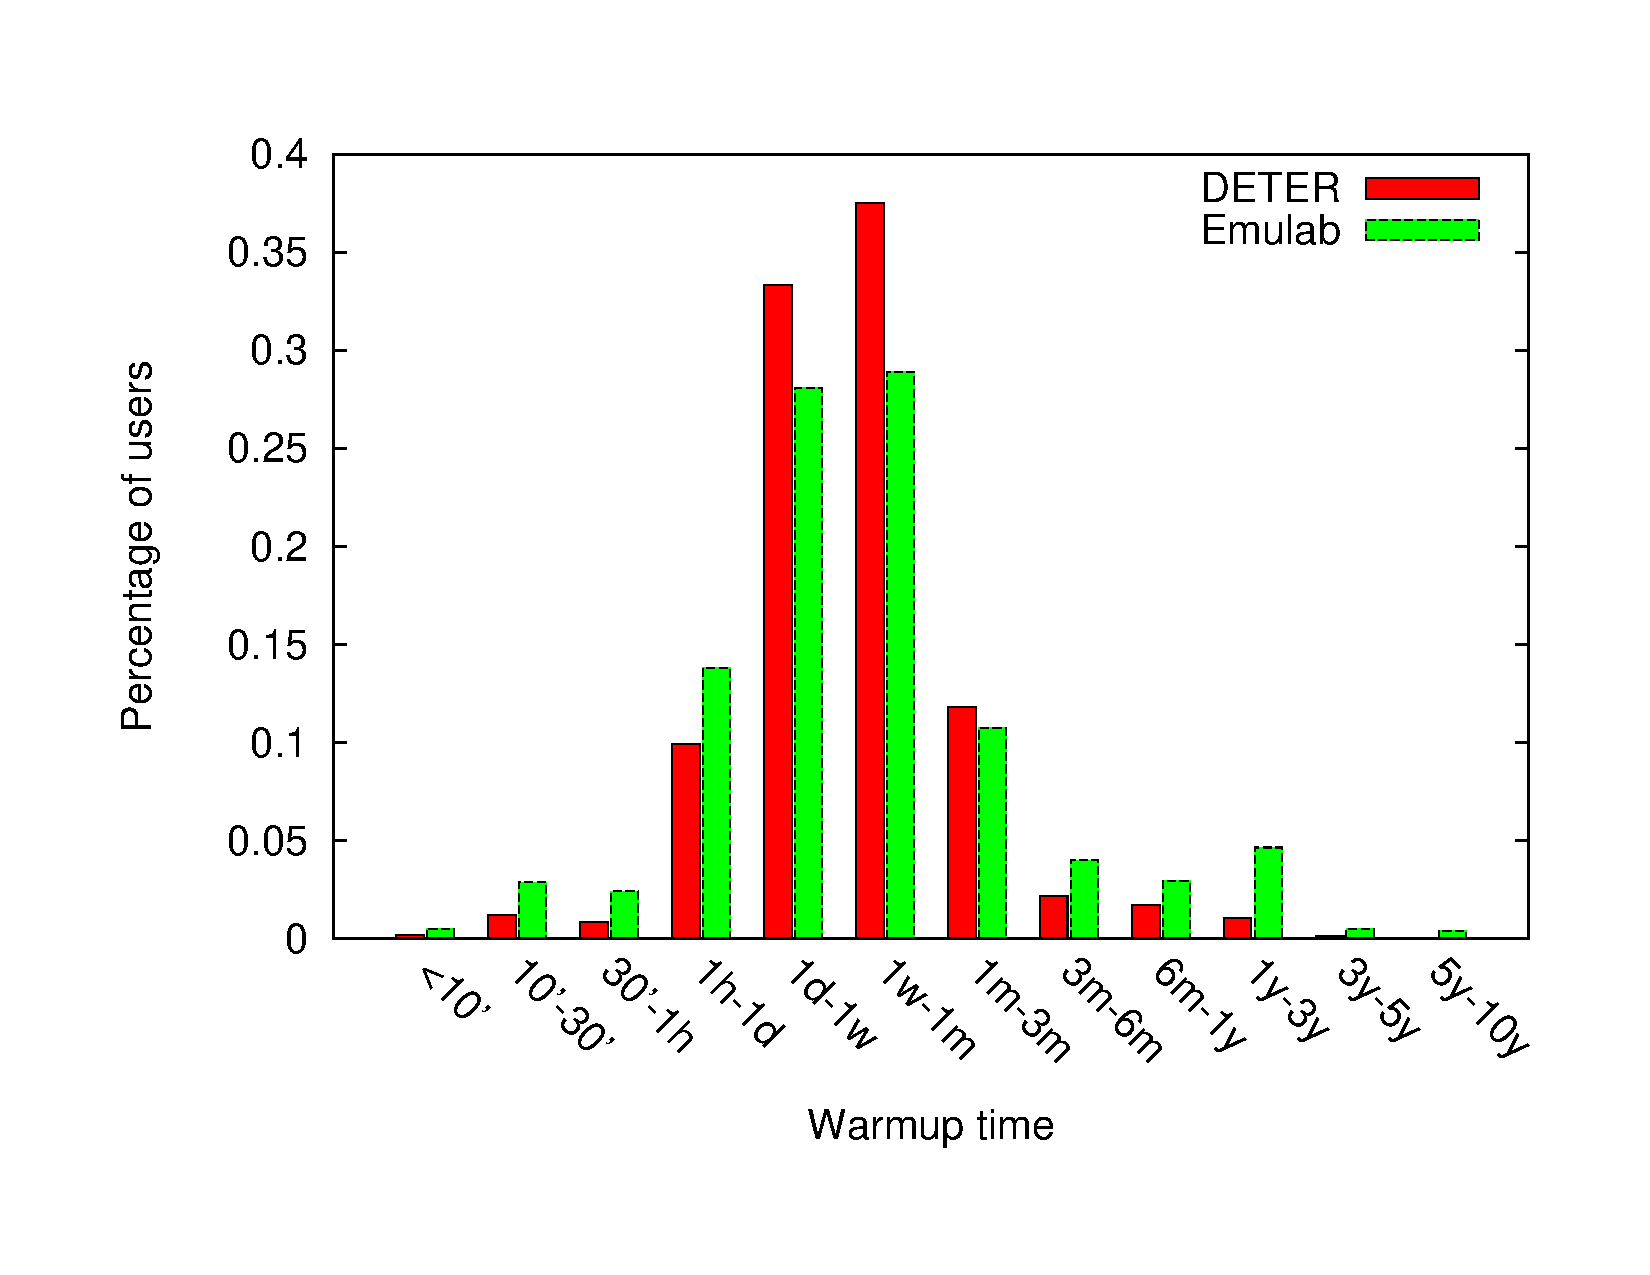
\includegraphics[width=3in]{figs/warmup_user.pdf} \caption{User warmup
time in DETER and Emulab} \label{warmupus} \end{center} \end{figure}

\begin{figure}[htbp] \begin{center}
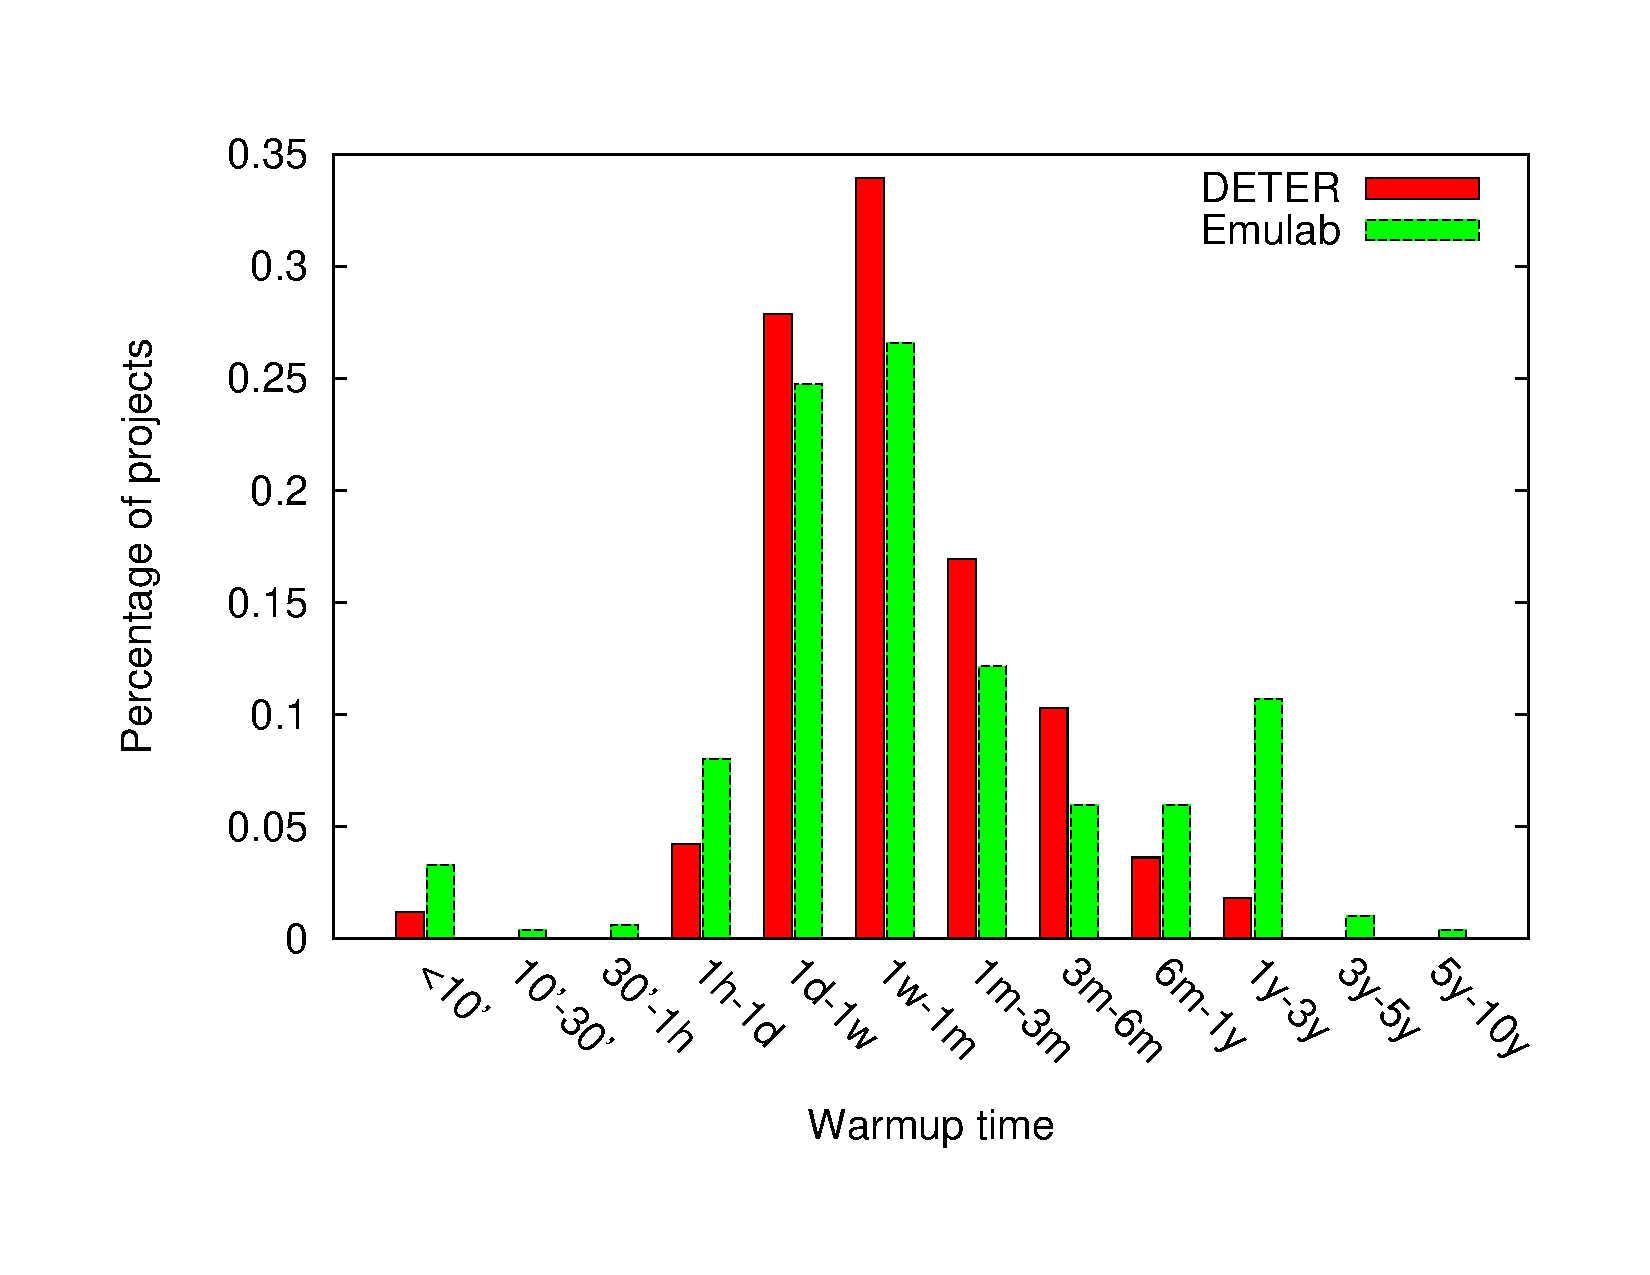
\includegraphics[width=3in]{figs/warmup_proj.pdf} \caption{Project
warmup time in DETER and Emulab} \label{warmuppr} \end{center}
\end{figure}


\begin{figure}[htbp] \begin{center}
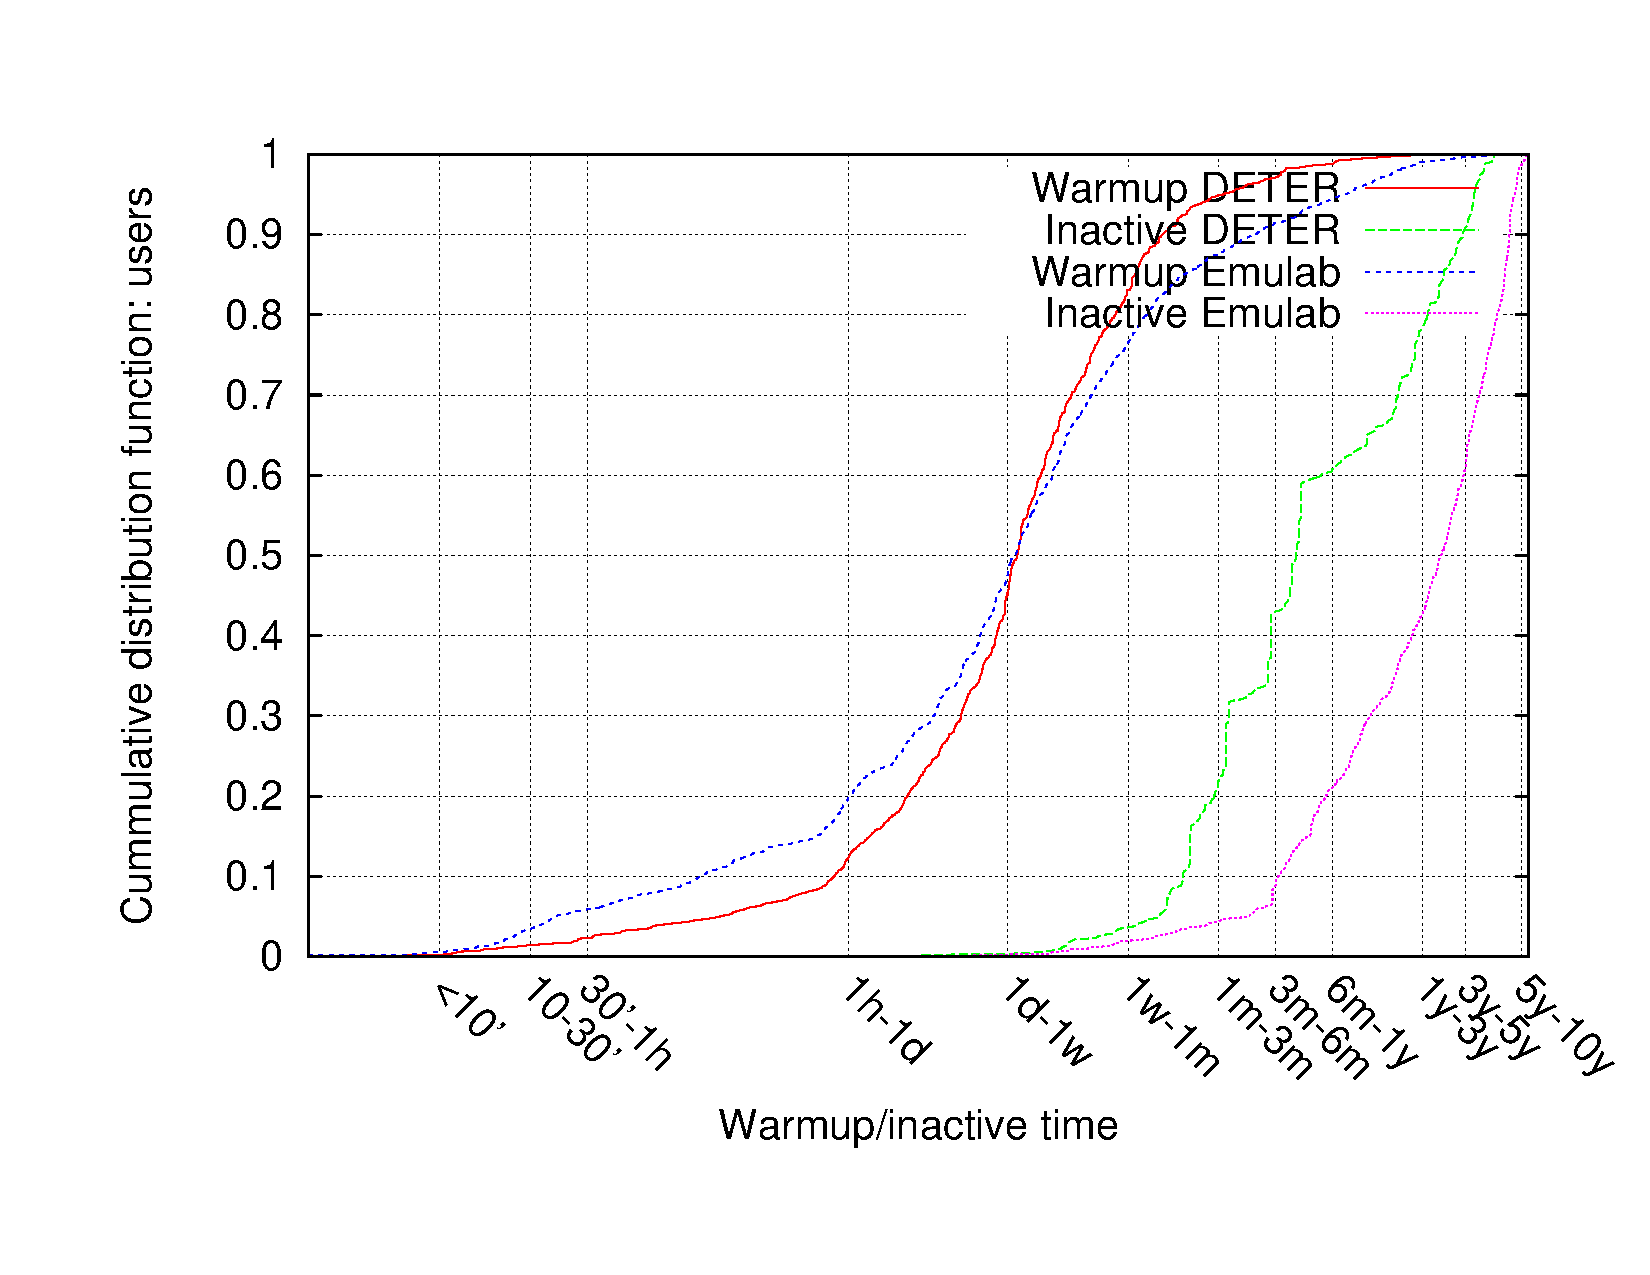
\includegraphics[width=3in]{figs/warmup_inact_user.pdf} \caption{User
warmup and inactive time} \label{warmupinus} \end{center} \end{figure}


\begin{figure}[htbp] \begin{center}
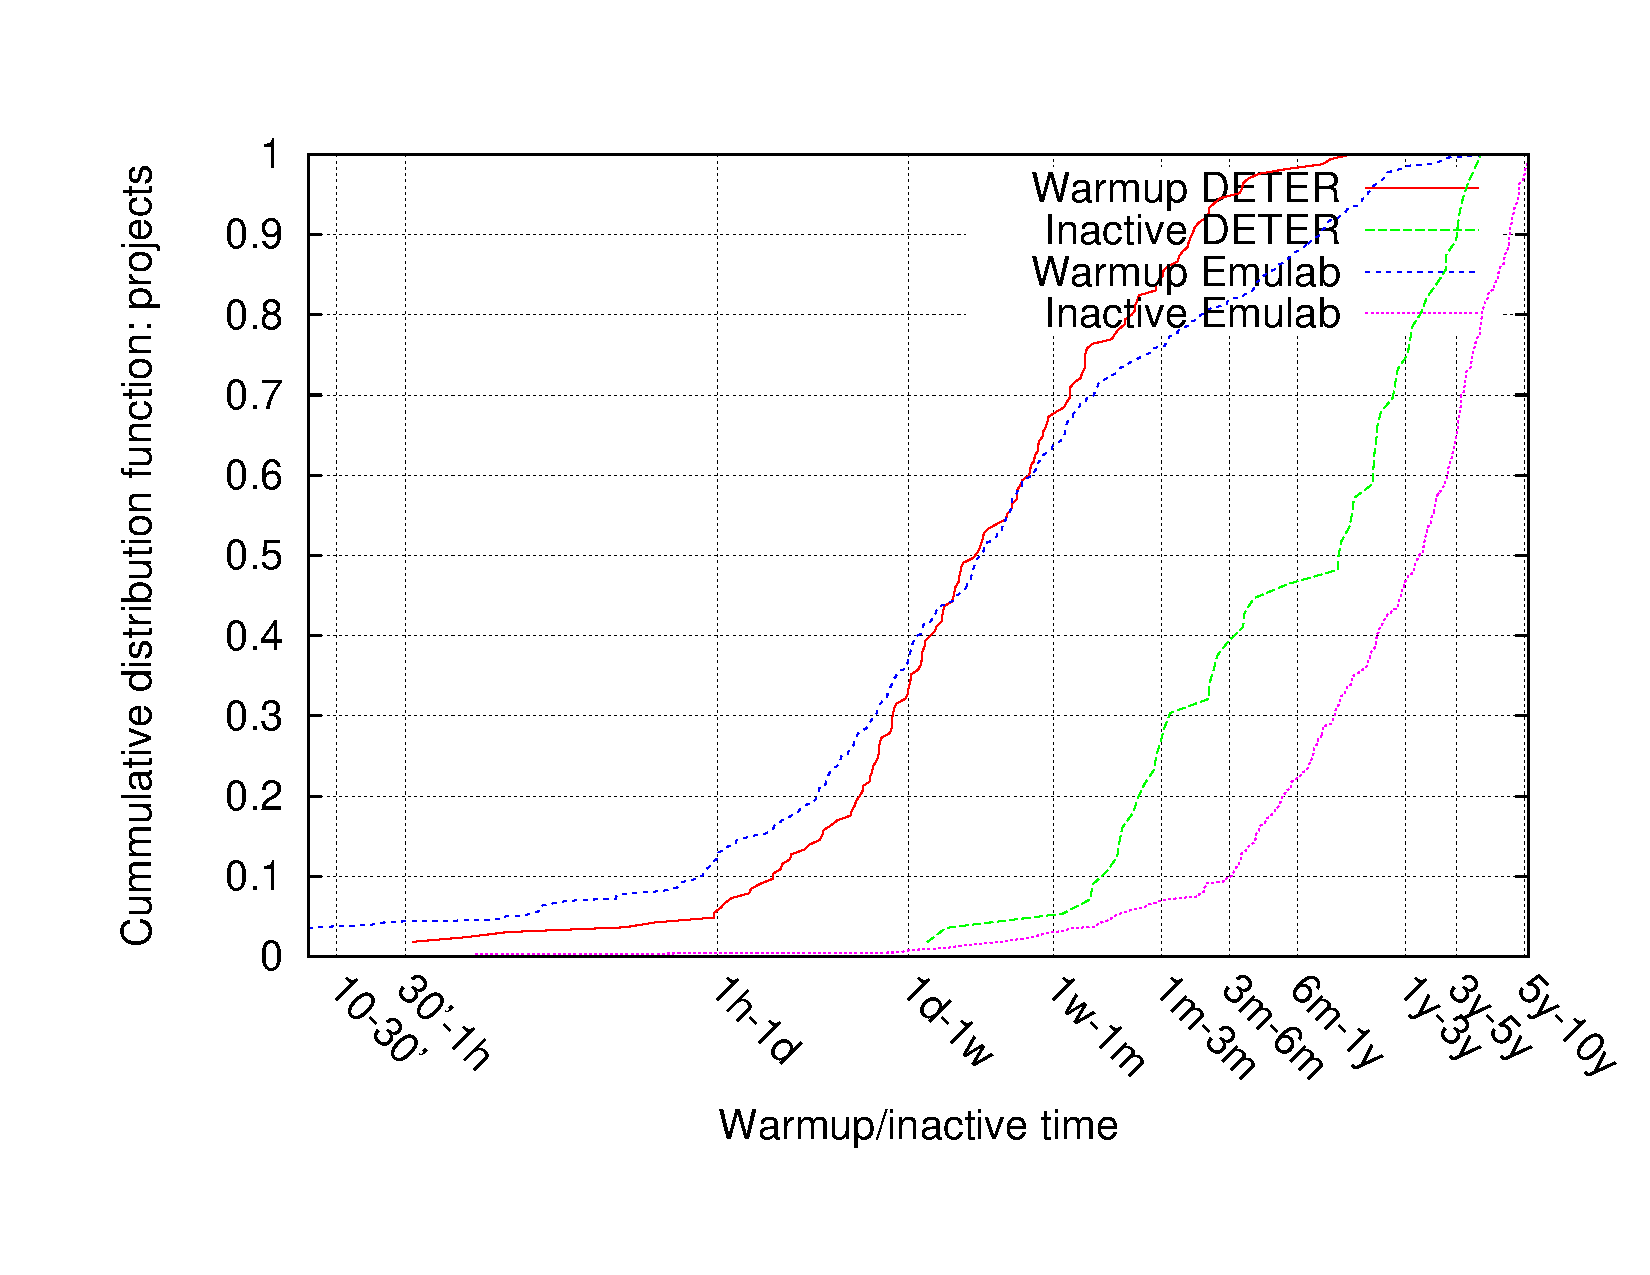
\includegraphics[width=3in]{figs/warmup_inact_proj.pdf} \caption{Project
warmup and inactive time} \label{warmupinpr} \end{center} \end{figure}

If we use the maximum value of the warmup time for the threshold then
the starred rows in the table \ref{cleaning} apply.

We now look at number of projects per research category. This is shown
in table \ref{projrc}. We took DDoS, worm and botnet out of attack
category because they are popular topics in recent years.

\begin{table}[htdp] \begin{center} \begin{tabular}{|c|c|} \hline
Research category & Projects \\\hline Attacks & 48  \\ DDoS & 18 \\
Architecture & 14\\ Infrastructure & 12 \\ Testbeds & 12 \\ Worms & 11
\\ Evaluation & 8 \\ Privacy & 6 \\ Botnets & 4 \\ \hline \end{tabular}
\end{center} \caption{Projects per research category} \label{projrc}
\end{table}%


\section{Experiment Patterns}

Say exps from outcome projects follow same trends as all so we don't
show them here.

\begin{figure}[htbp] \begin{center}
\includegraphics[width=3in,type=pdf,ext=.pdf,read=.pdf]{figs/exp.size.
gnu} \caption{Experiment instance size} \label{expsize} \end{center}
\end{figure}

\begin{figure}[htbp] \begin{center}
\includegraphics[width=3in,type=pdf,ext=.pdf,read=.pdf]{figs/planet.size
.gnu} \caption{Experiment instance size in Planetlab} \label{expsize}
\end{center} \end{figure}

\begin{figure}[htbp] \begin{center} 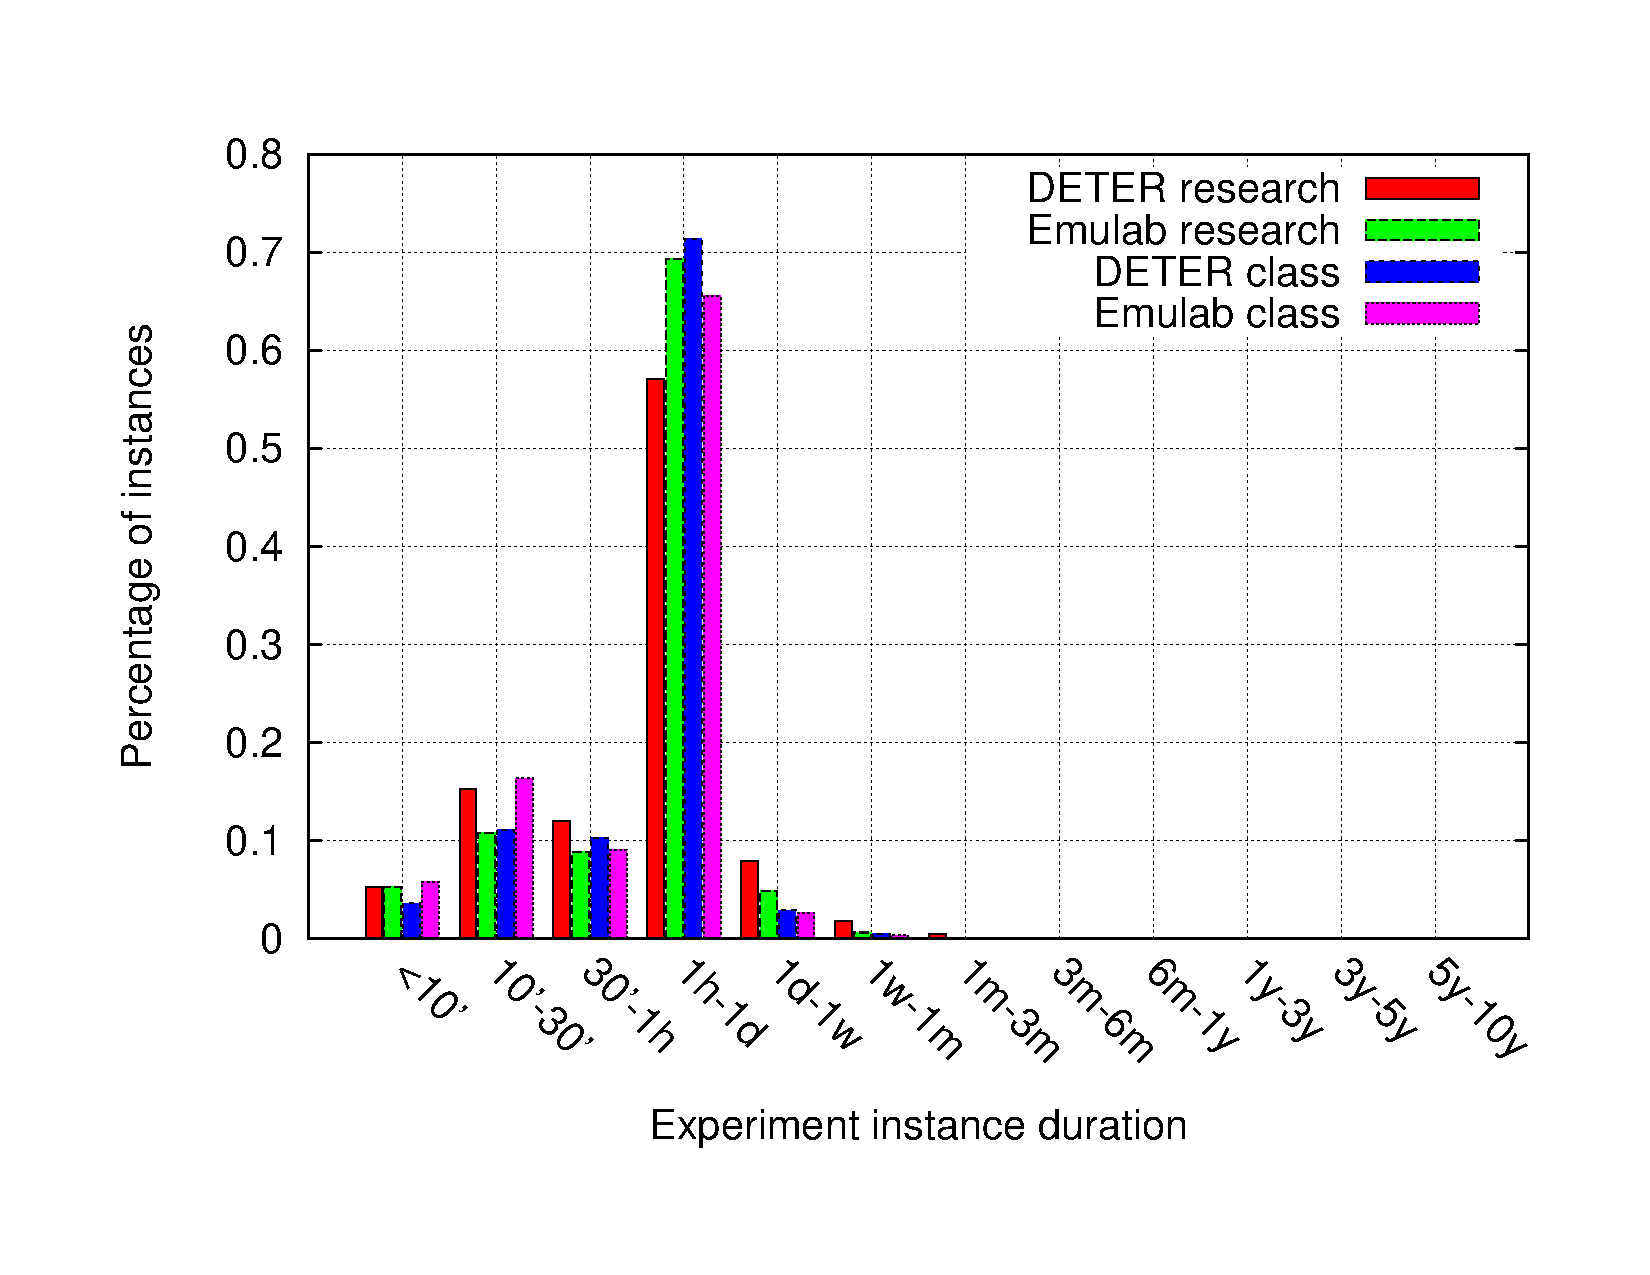
\includegraphics[width=3in,
type=pdf,ext=.pdf,read=.pdf]{figs/exp.dur.gnu} \caption{Experiment
instance duration} \label{expdur} \end{center} \end{figure}

\begin{figure}[htbp] \begin{center} 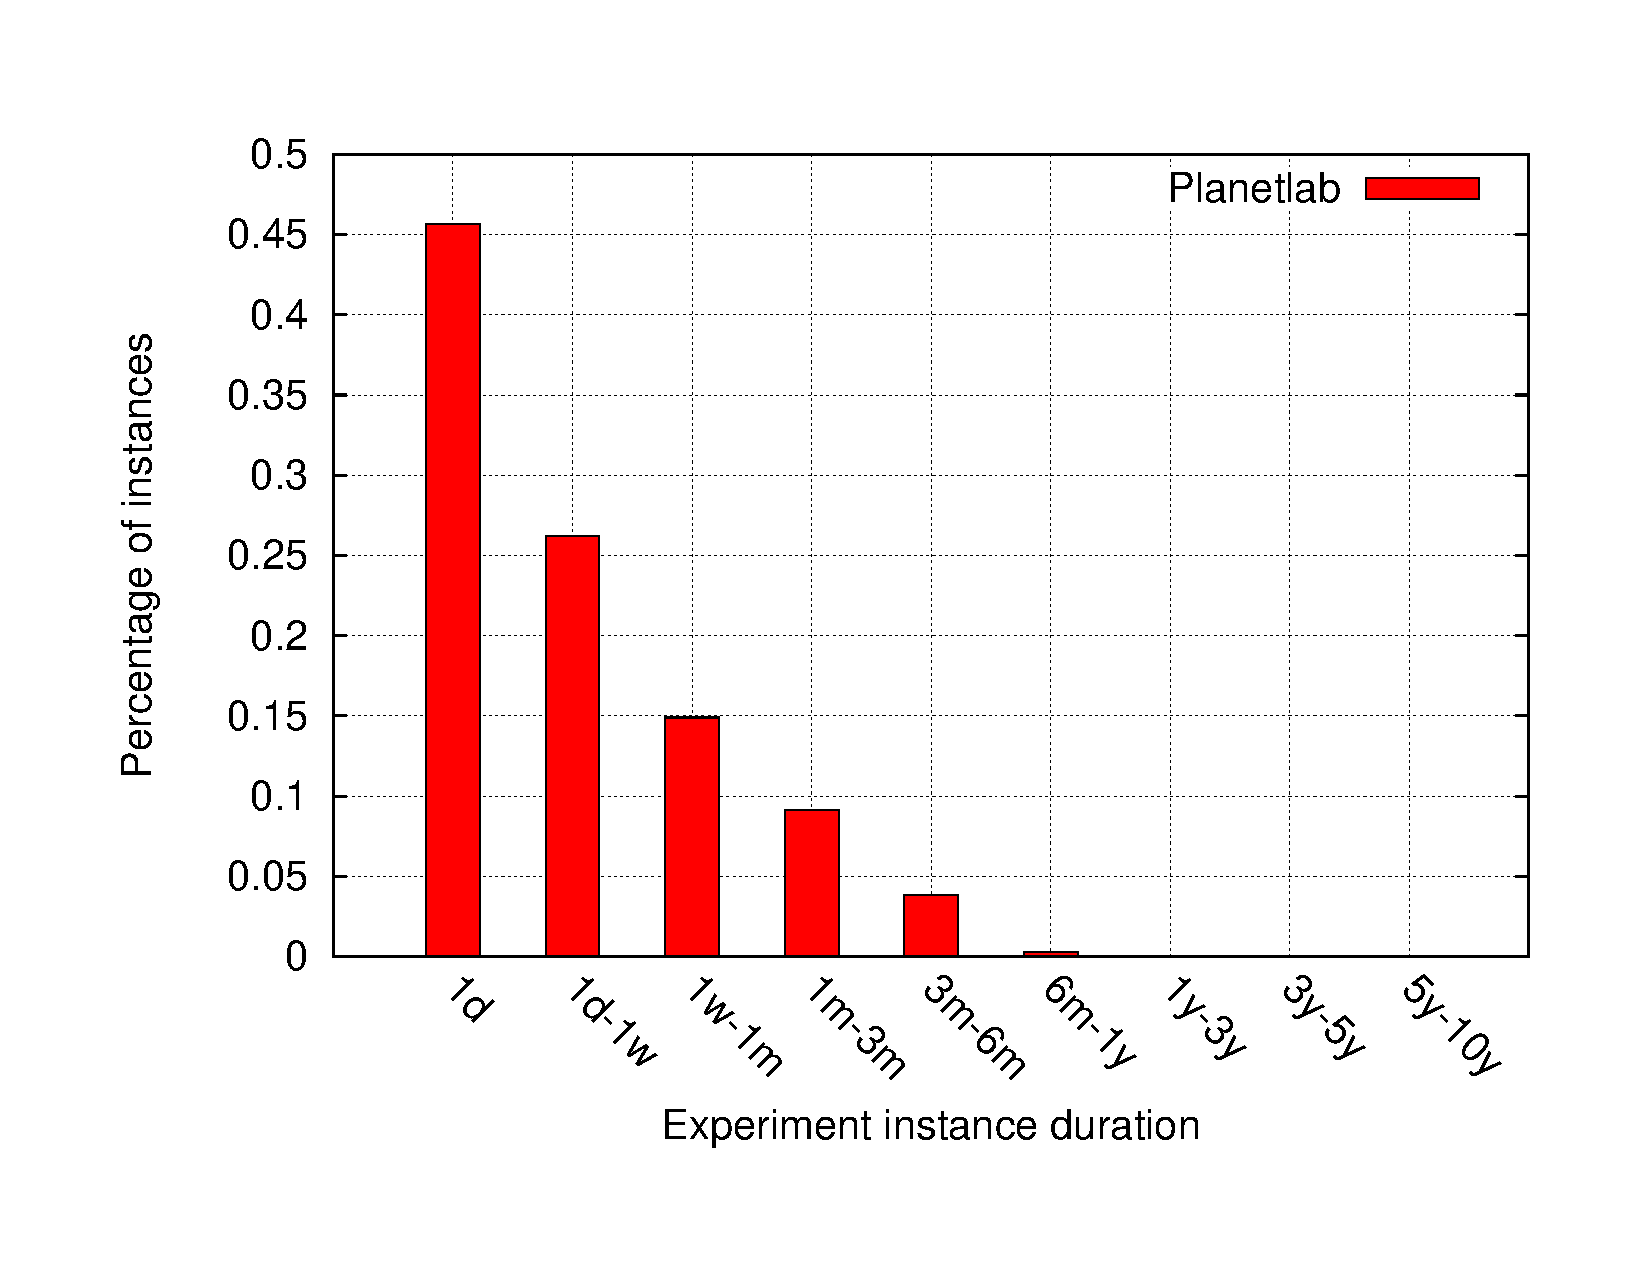
\includegraphics[width=3in,
type=pdf,ext=.pdf,read=.pdf]{figs/planet.dur.gnu} \caption{Experiment
instance duration in Planetlab} \label{expdur} \end{center} \end{figure}

\begin{figure}[htbp] \begin{center} 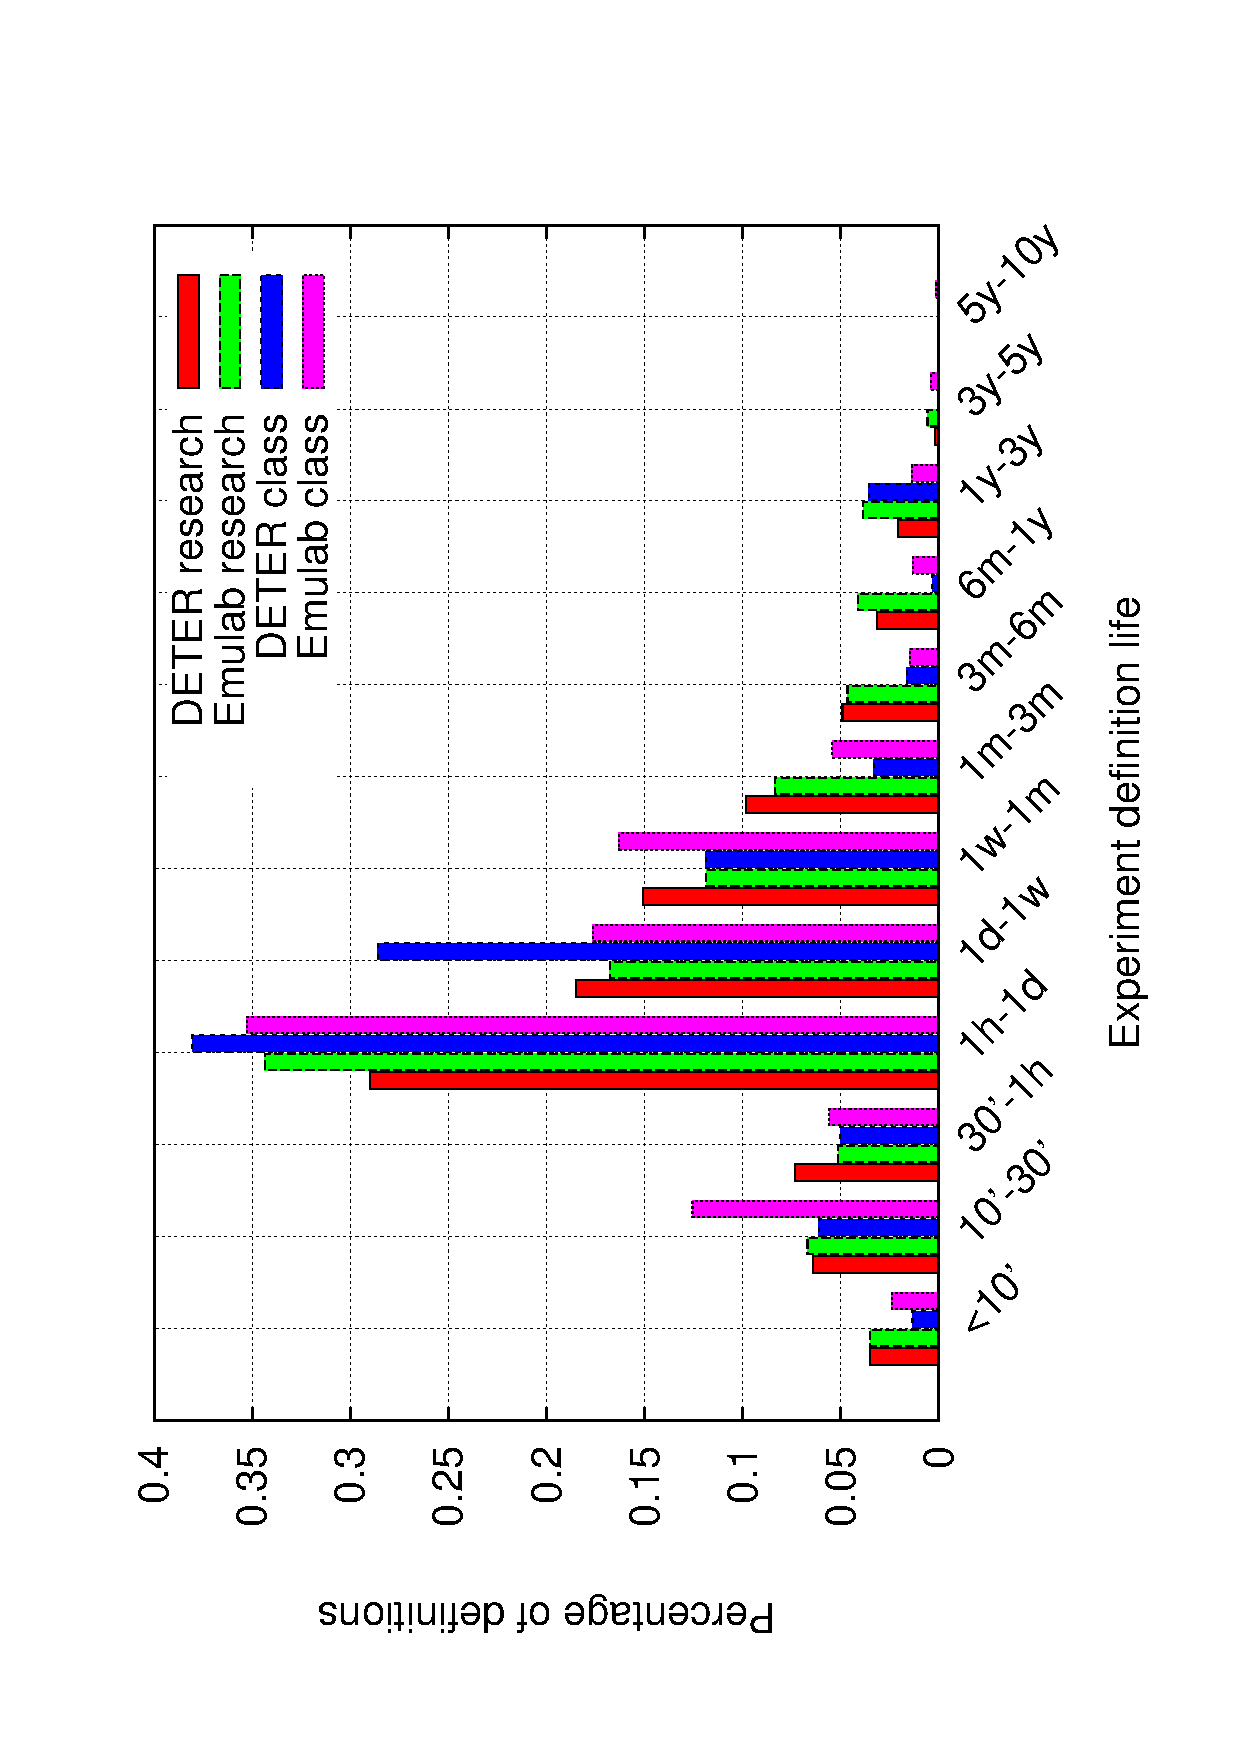
\includegraphics[width=3in,
type=pdf,ext=.pdf,read=.pdf]{figs/exp.life.gnu} \caption{Experiment
definition life} \label{explife} \end{center} \end{figure}

\begin{figure}[htbp] \begin{center} 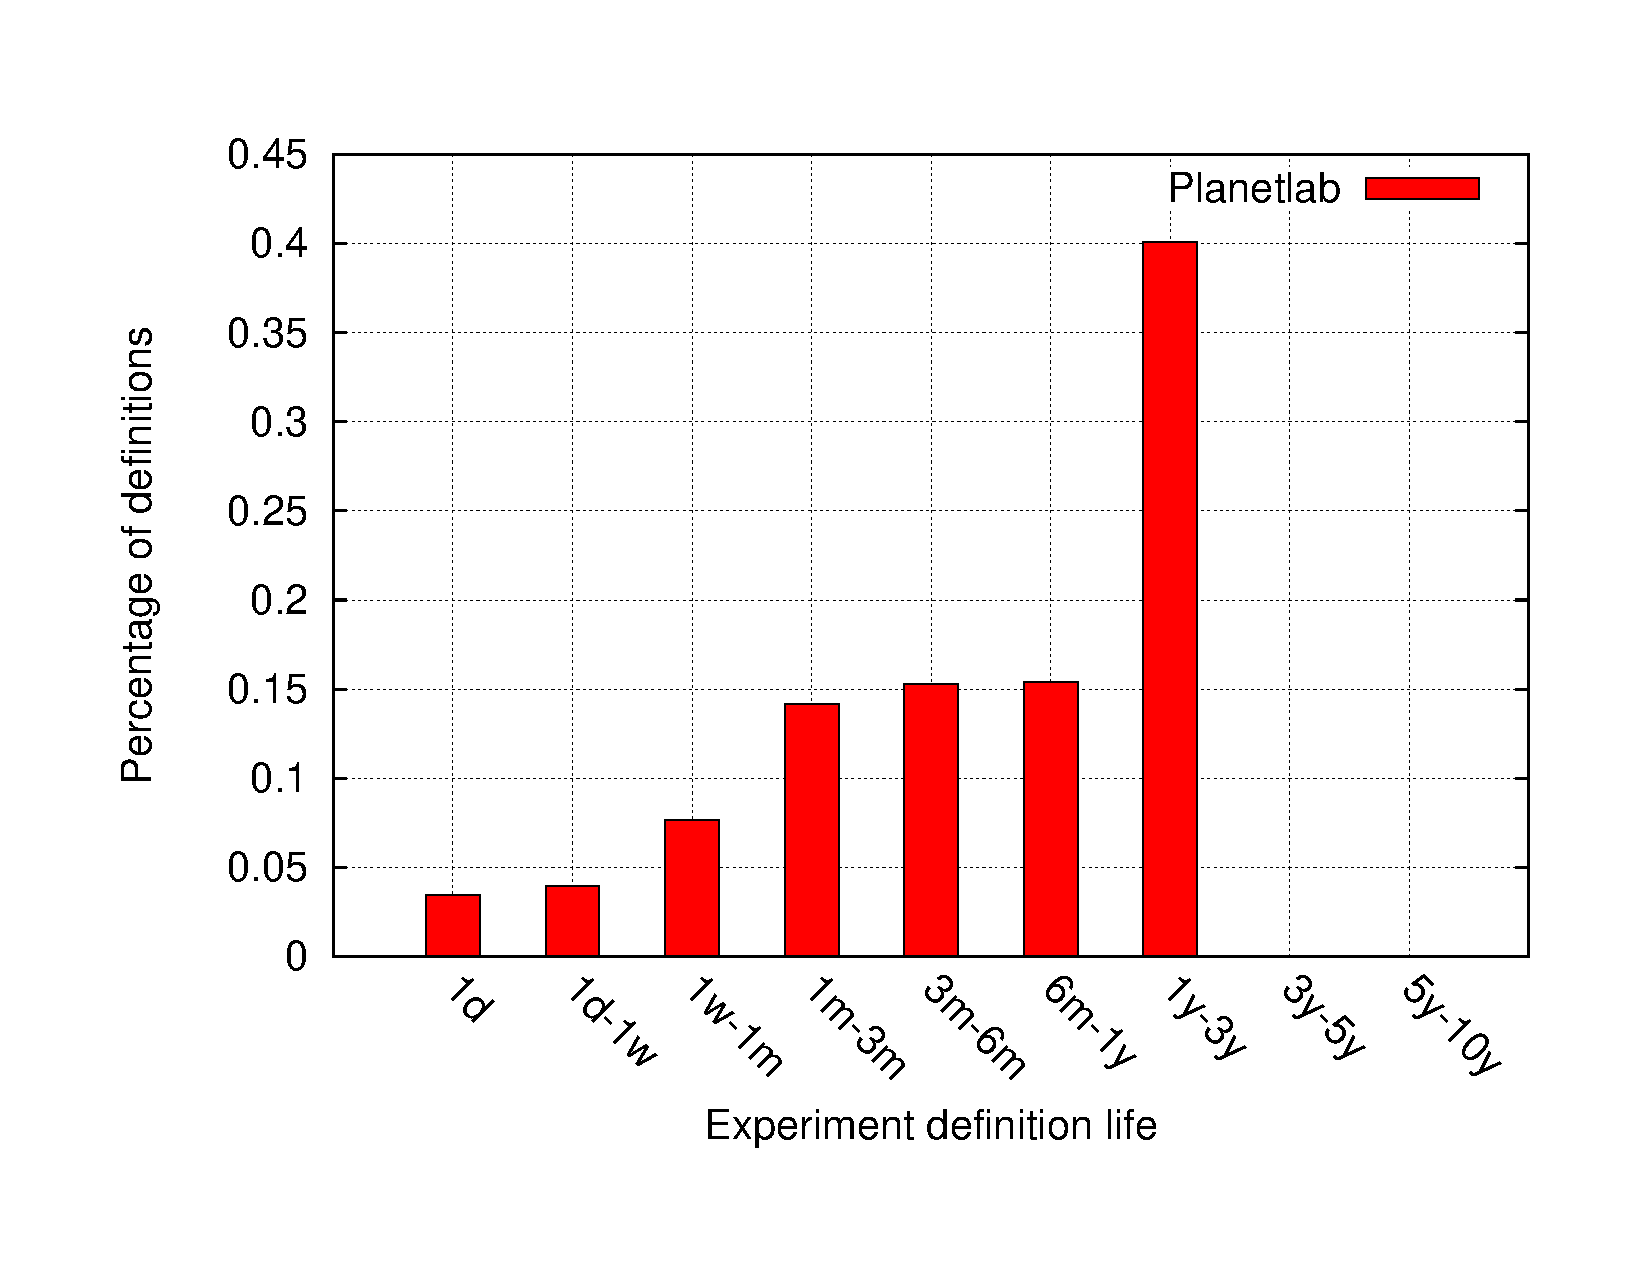
\includegraphics[width=3in,
type=pdf,ext=.pdf,read=.pdf]{figs/planet.life.gnu} \caption{Experiment
definition life in Planetlab} \label{explife} \end{center} \end{figure}

\begin{figure}[htbp] \begin{center} 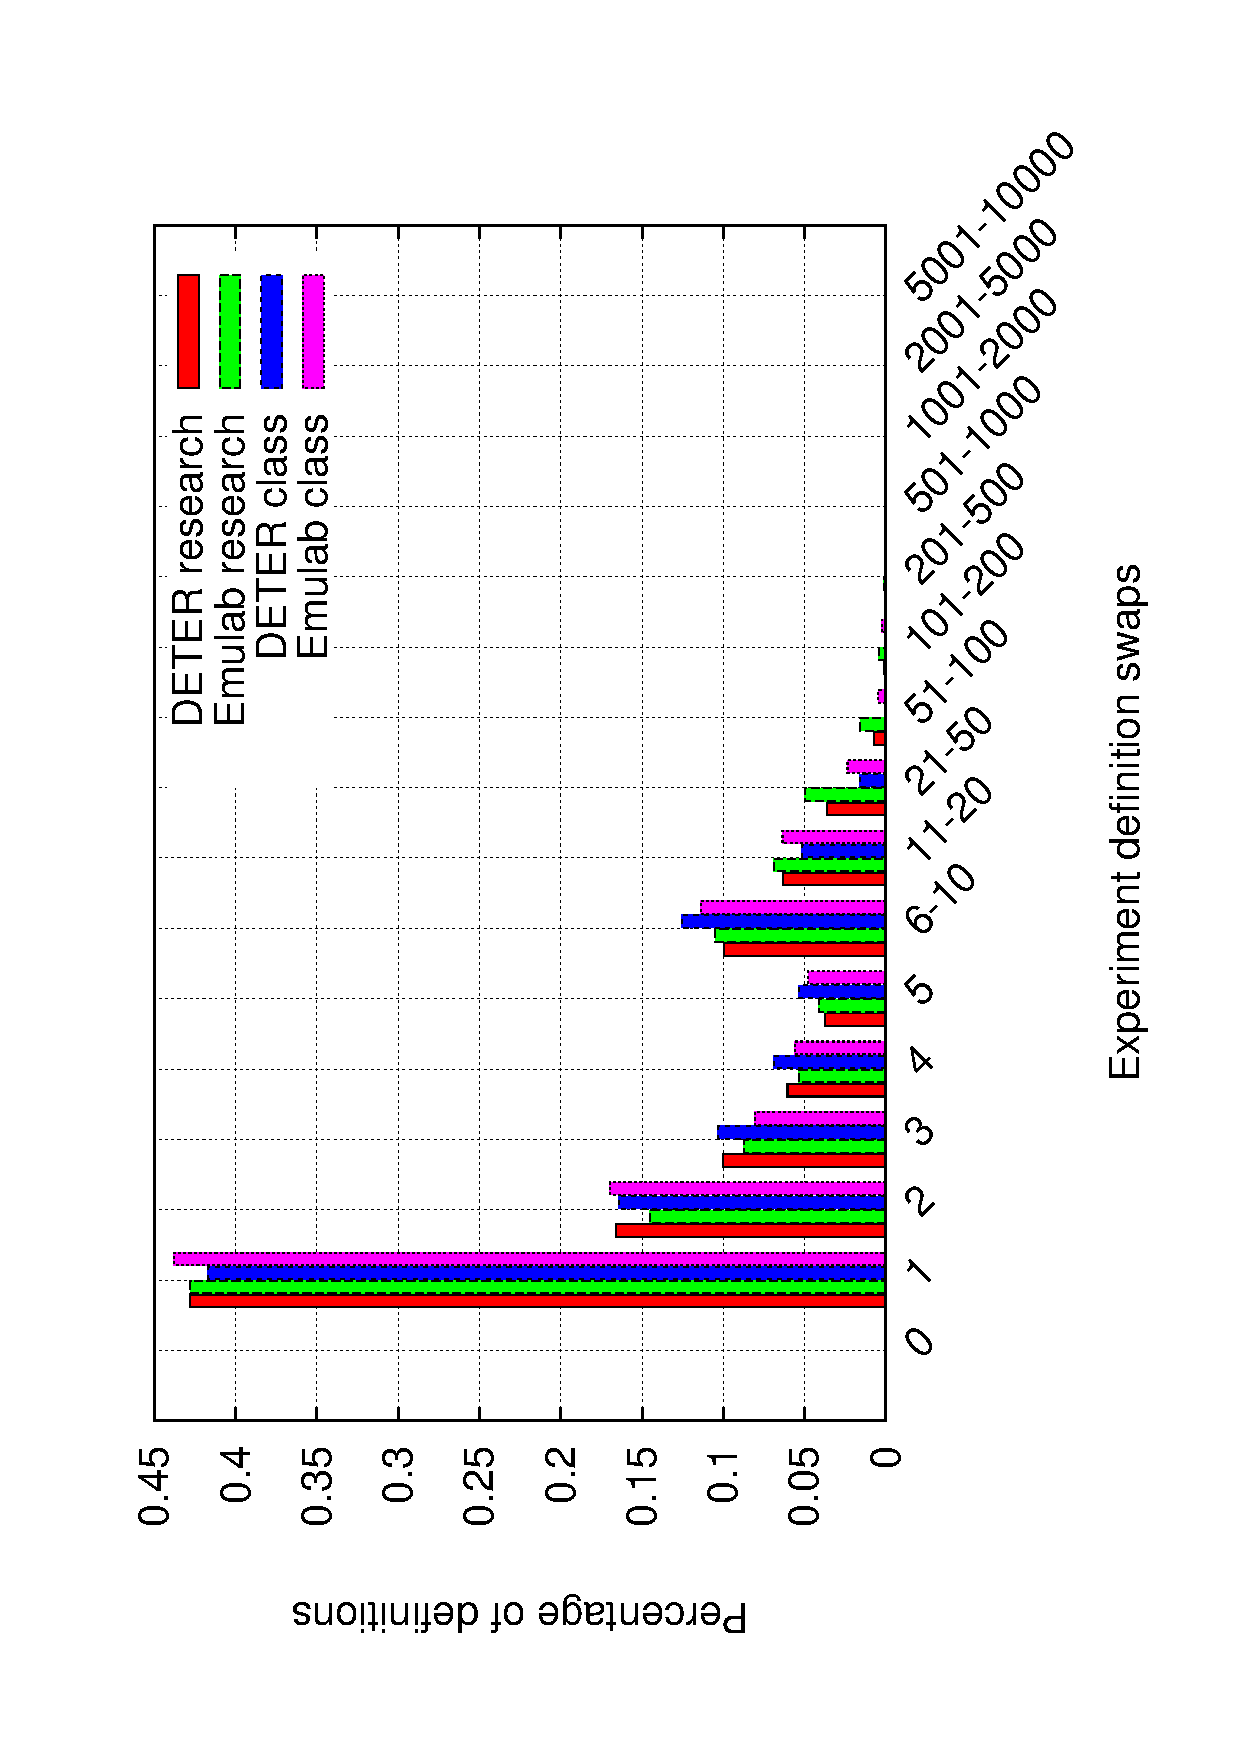
\includegraphics[width=3in,
type=pdf,ext=.pdf,read=.pdf]{figs/exp.swaps.gnu} \caption{Experiment
definition swaps} \label{expswaps} \end{center} \end{figure}

\begin{figure}[htbp] \begin{center} 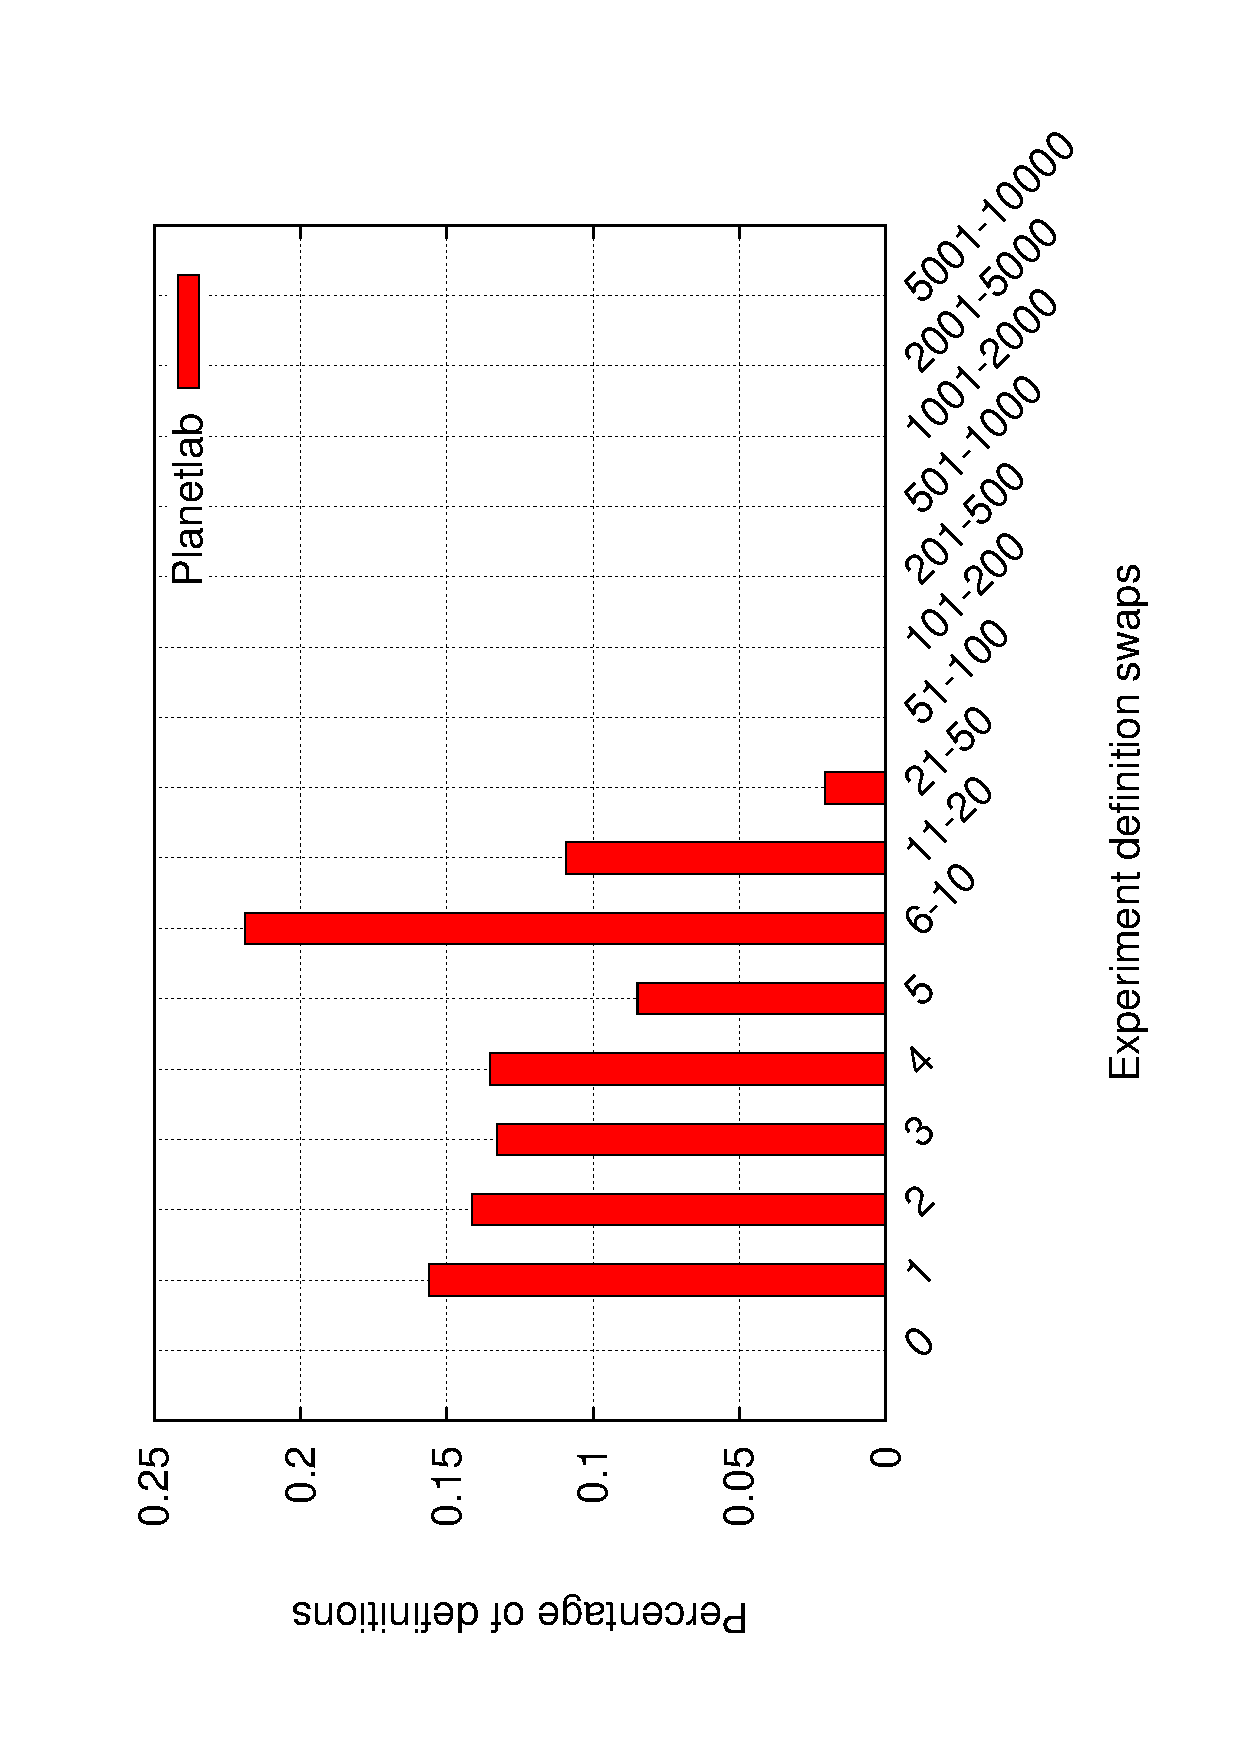
\includegraphics[width=3in,
type=pdf,ext=.pdf,read=.pdf]{figs/planet.swaps.gnu} \caption{Experiment
definition swaps in Planetlab} \label{expswaps} \end{center}
\end{figure}

\begin{figure*}[htbp] \begin{center} 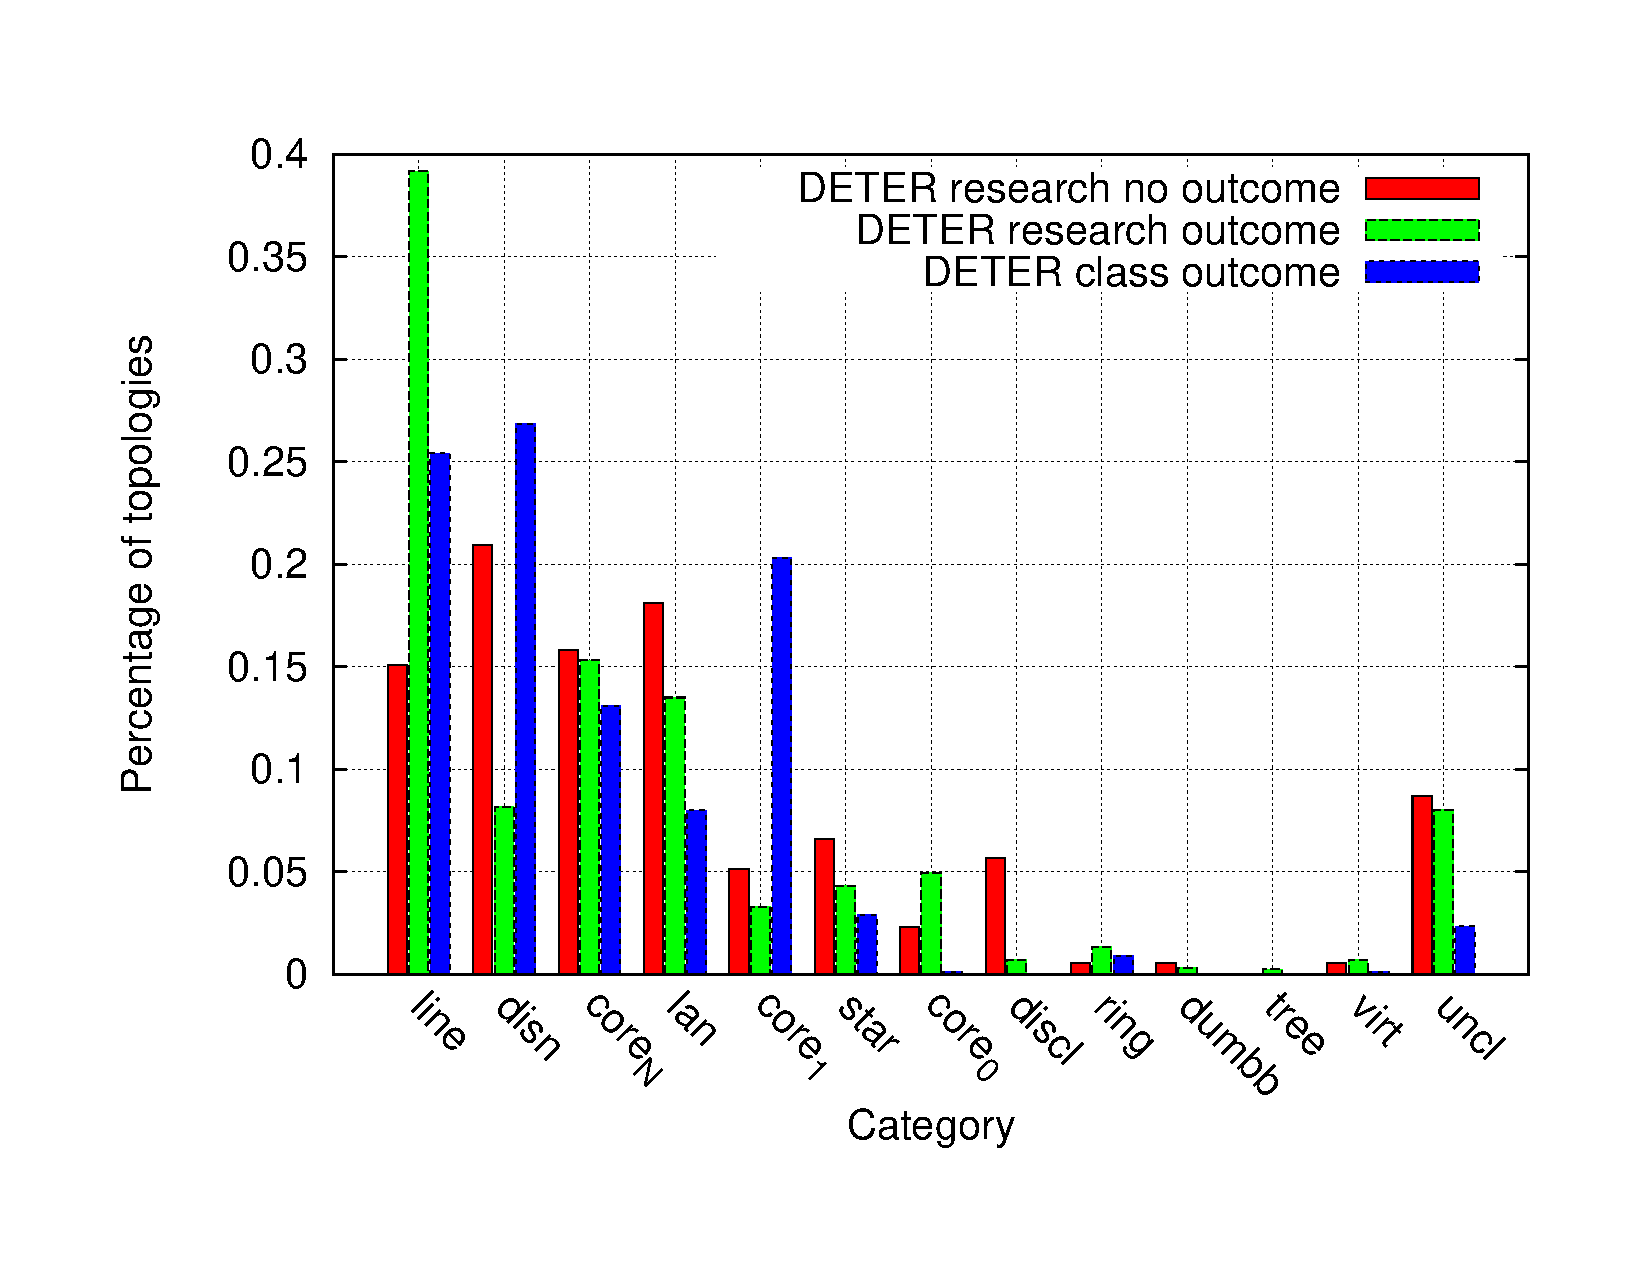
\includegraphics[width=3in,
type=pdf,ext=.pdf,read=.pdf]{figs/topo.gnu} 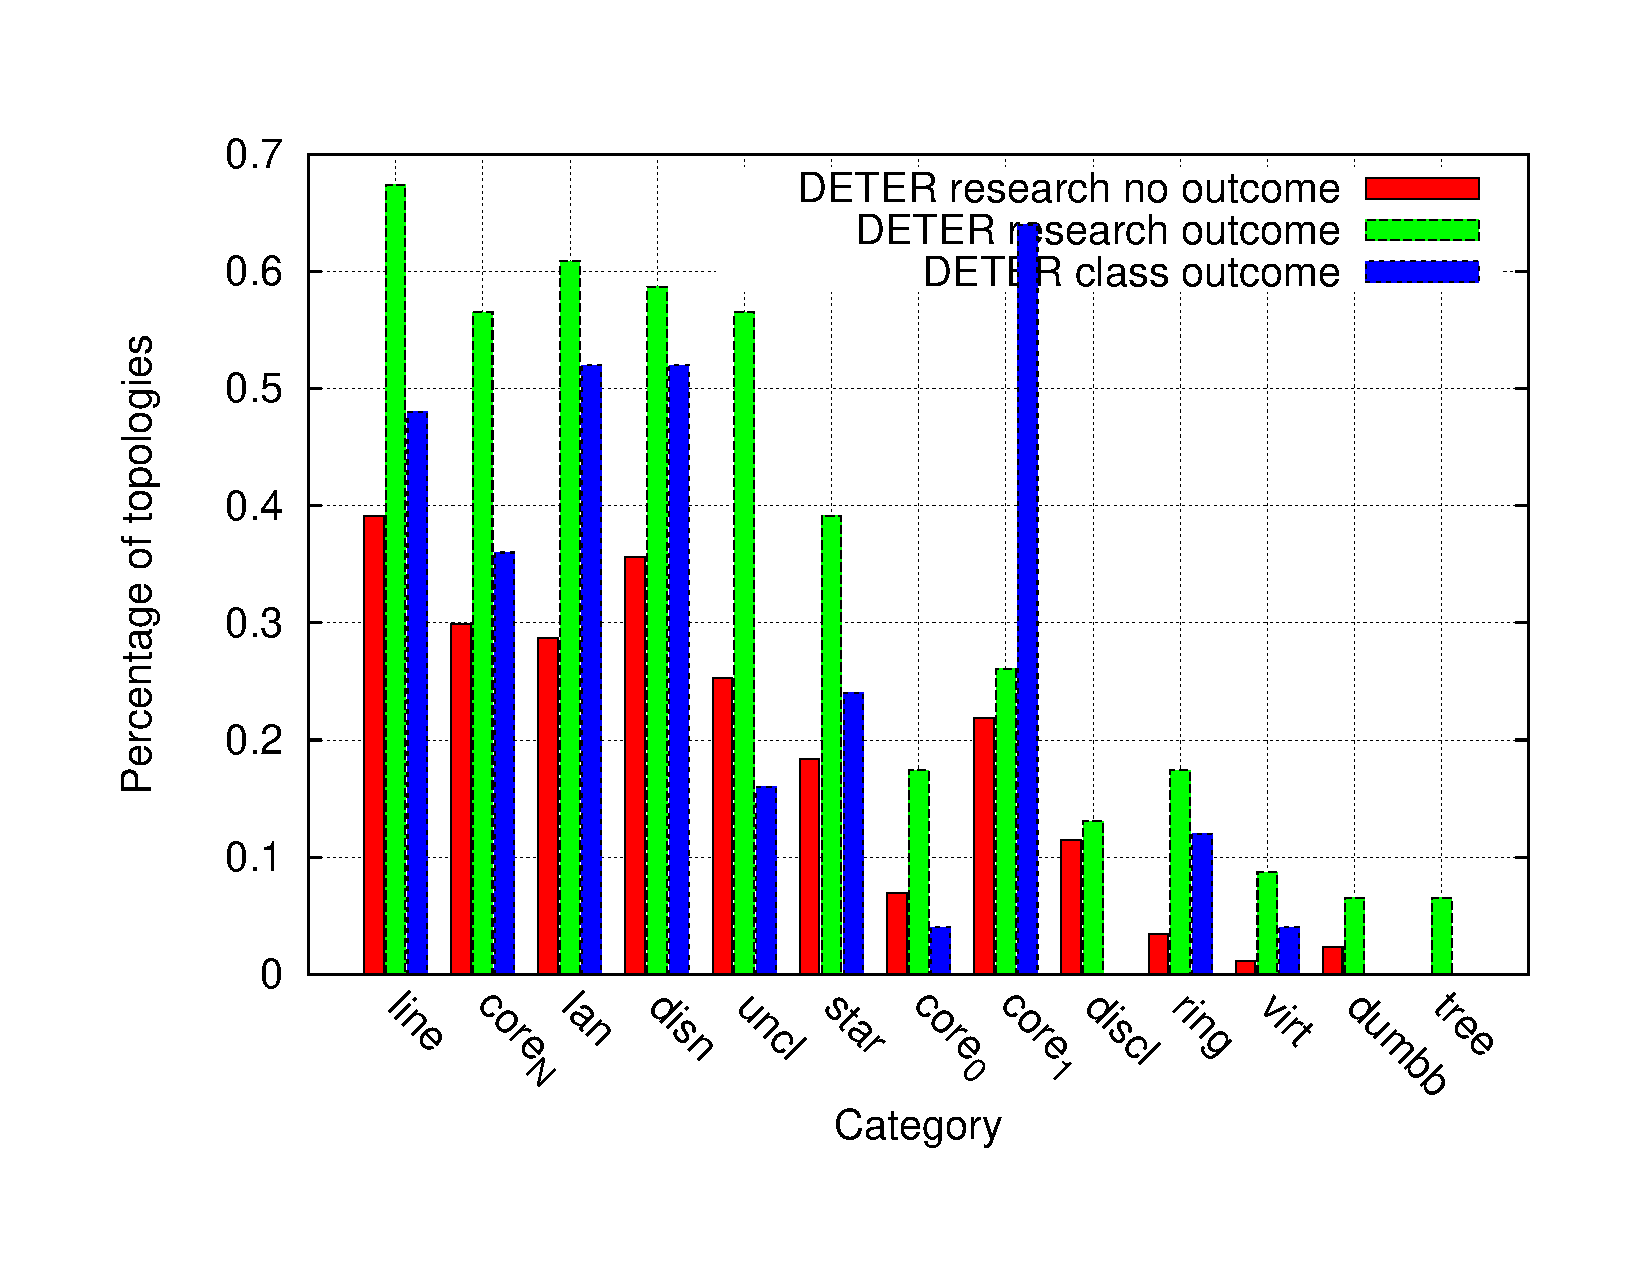
\includegraphics[width=3in,
type=pdf,ext=.pdf,read=.pdf]{figs/topop.gnu} \caption{Experiment
topologies in DETER: experiment vs project distribution} \label{topo}
\end{center} \end{figure*}




\section{Project Patterns}

In this case trends differ between all and outcome projects. Those with
outcome are definitely more active. \begin{figure*}[htbp] \begin{center}
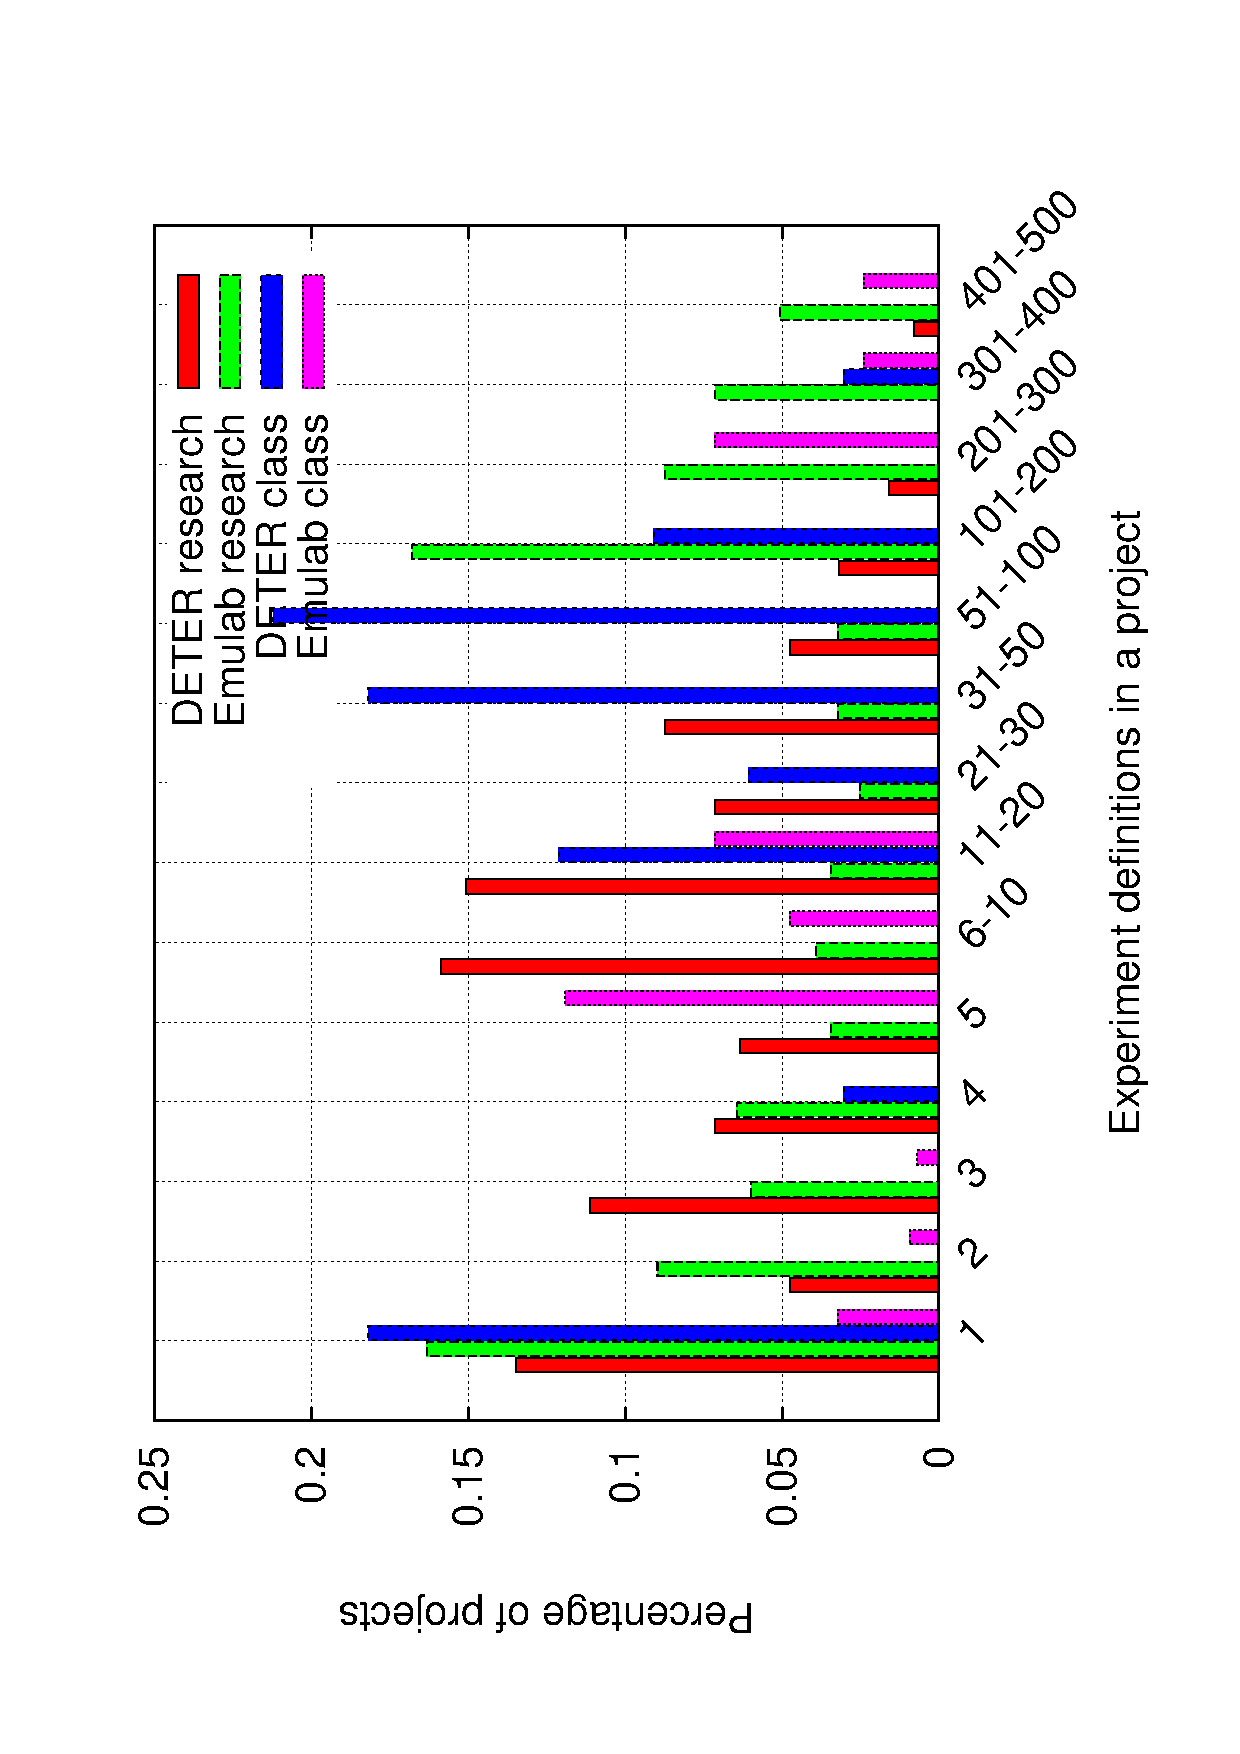
\includegraphics[width=3in,
type=pdf,ext=.pdf,read=.pdf]{figs/proj.size.gnu}
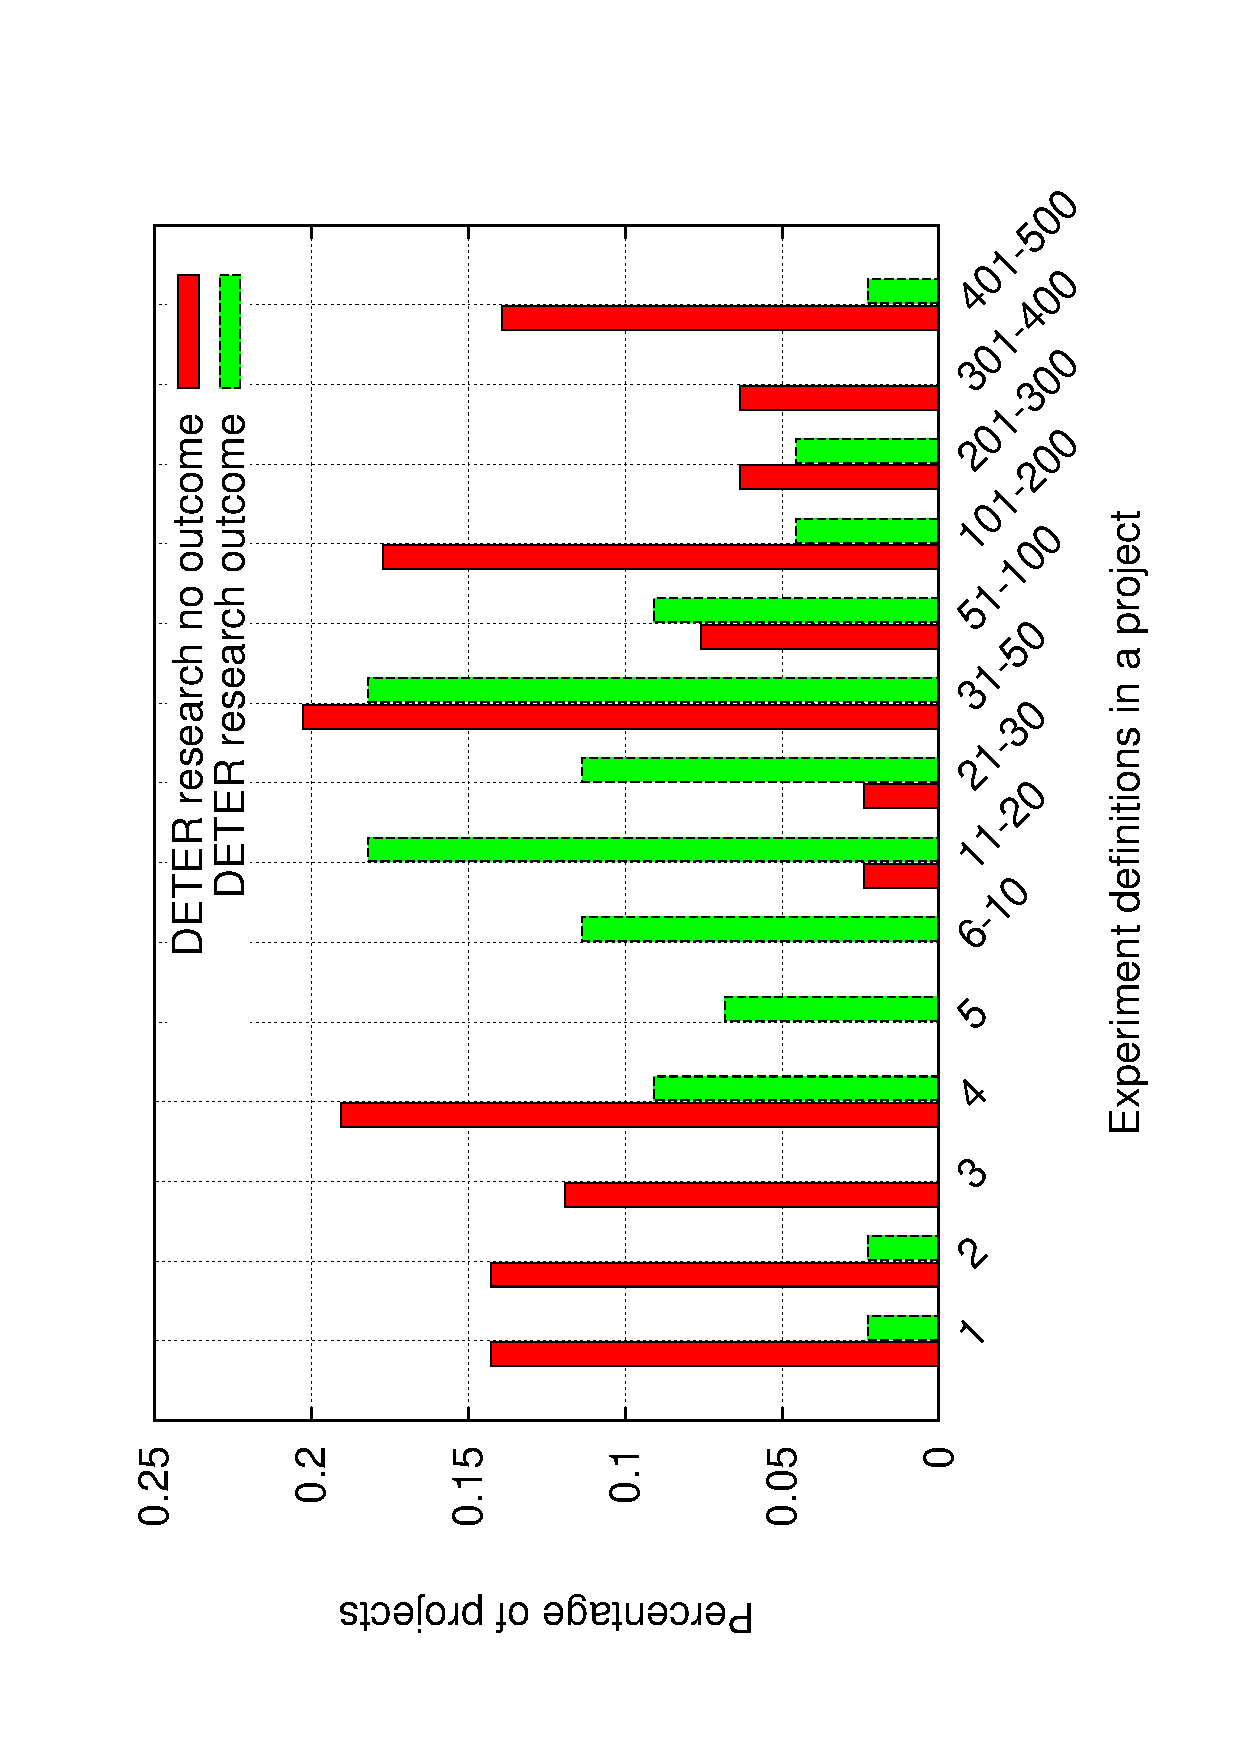
\includegraphics[width=3in,
type=pdf,ext=.pdf,read=.pdf]{figs/proj.size.cmp.gnu}
\caption{Experiments per project. Left: DETER vs Emulab, Right: All vs
outcome} \label{projsize} \end{center} \end{figure*}

\begin{figure*}[htbp] \begin{center} 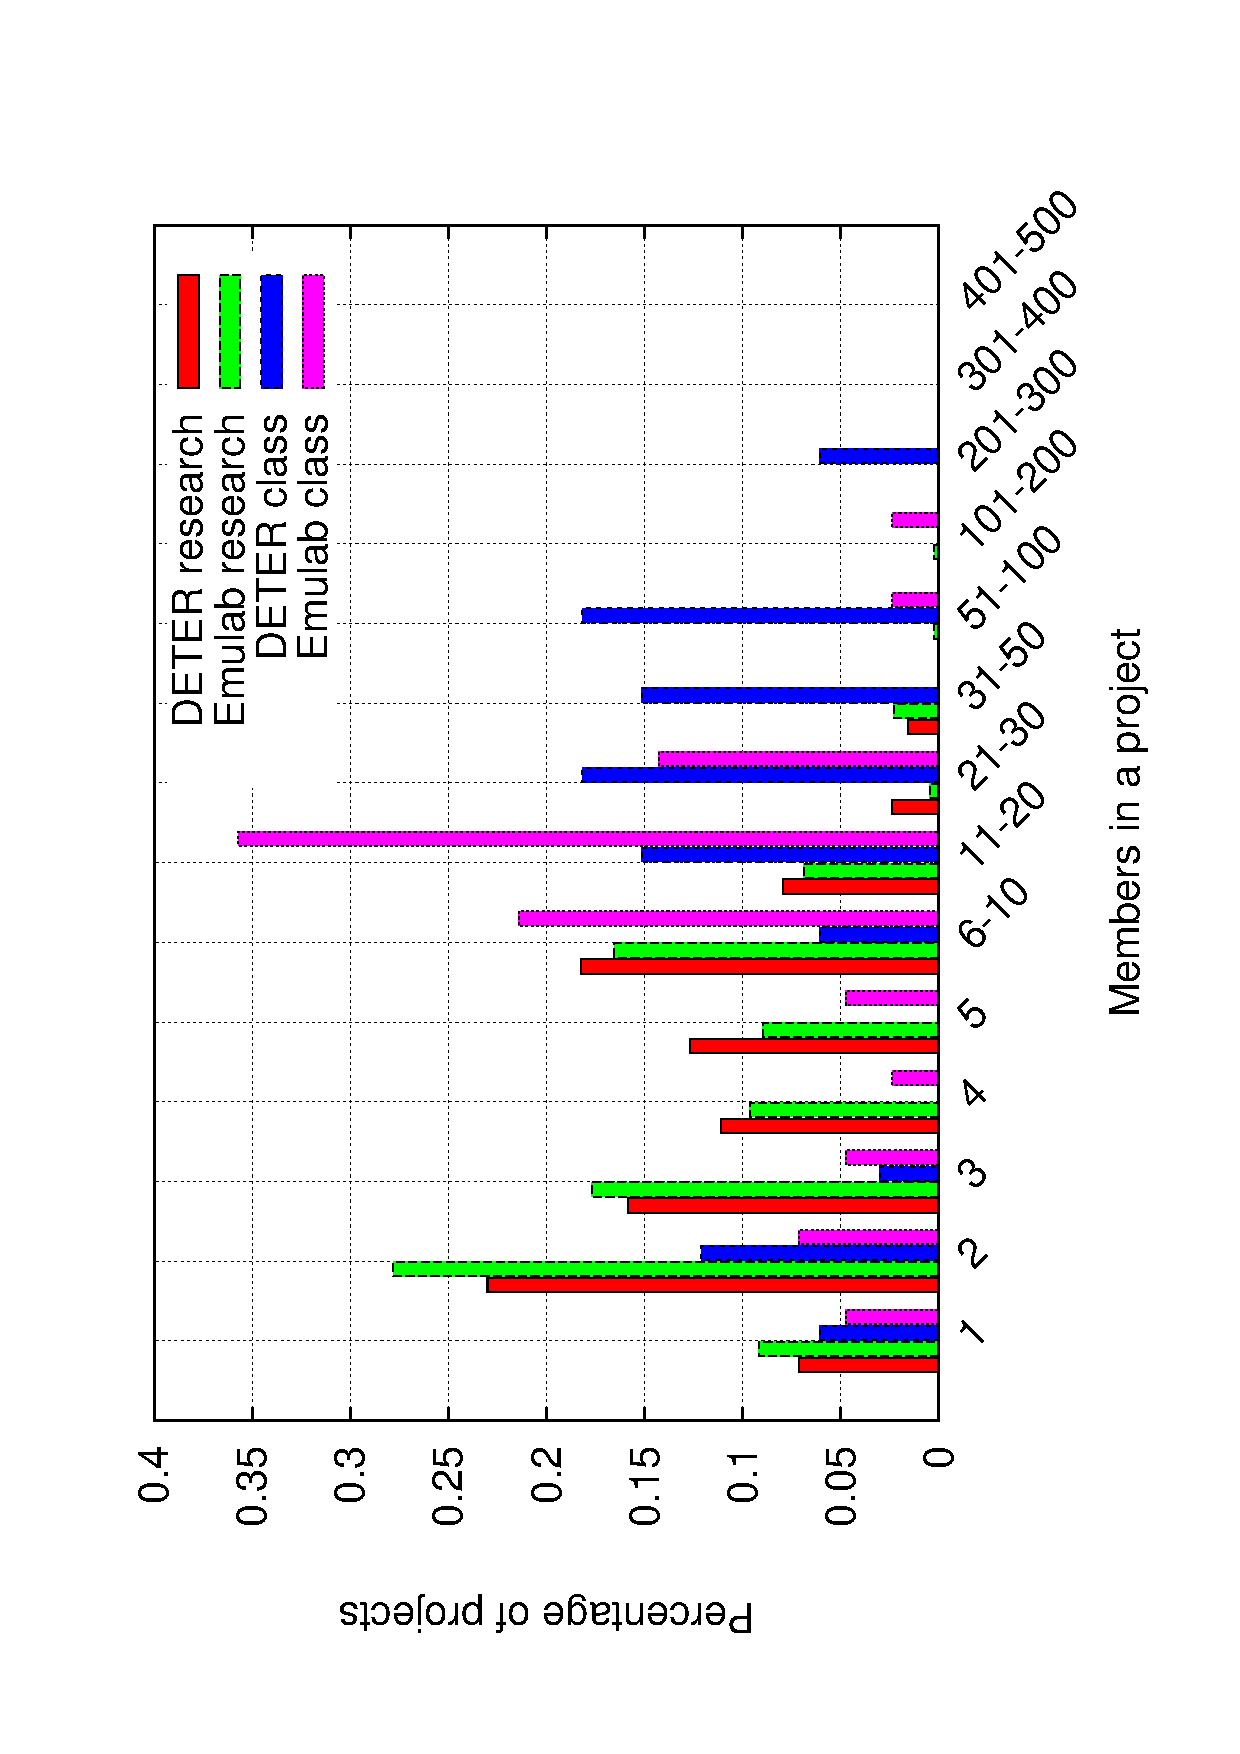
\includegraphics[width=3in,
type=pdf,ext=.pdf,read=.pdf]{figs/proj.user.gnu}
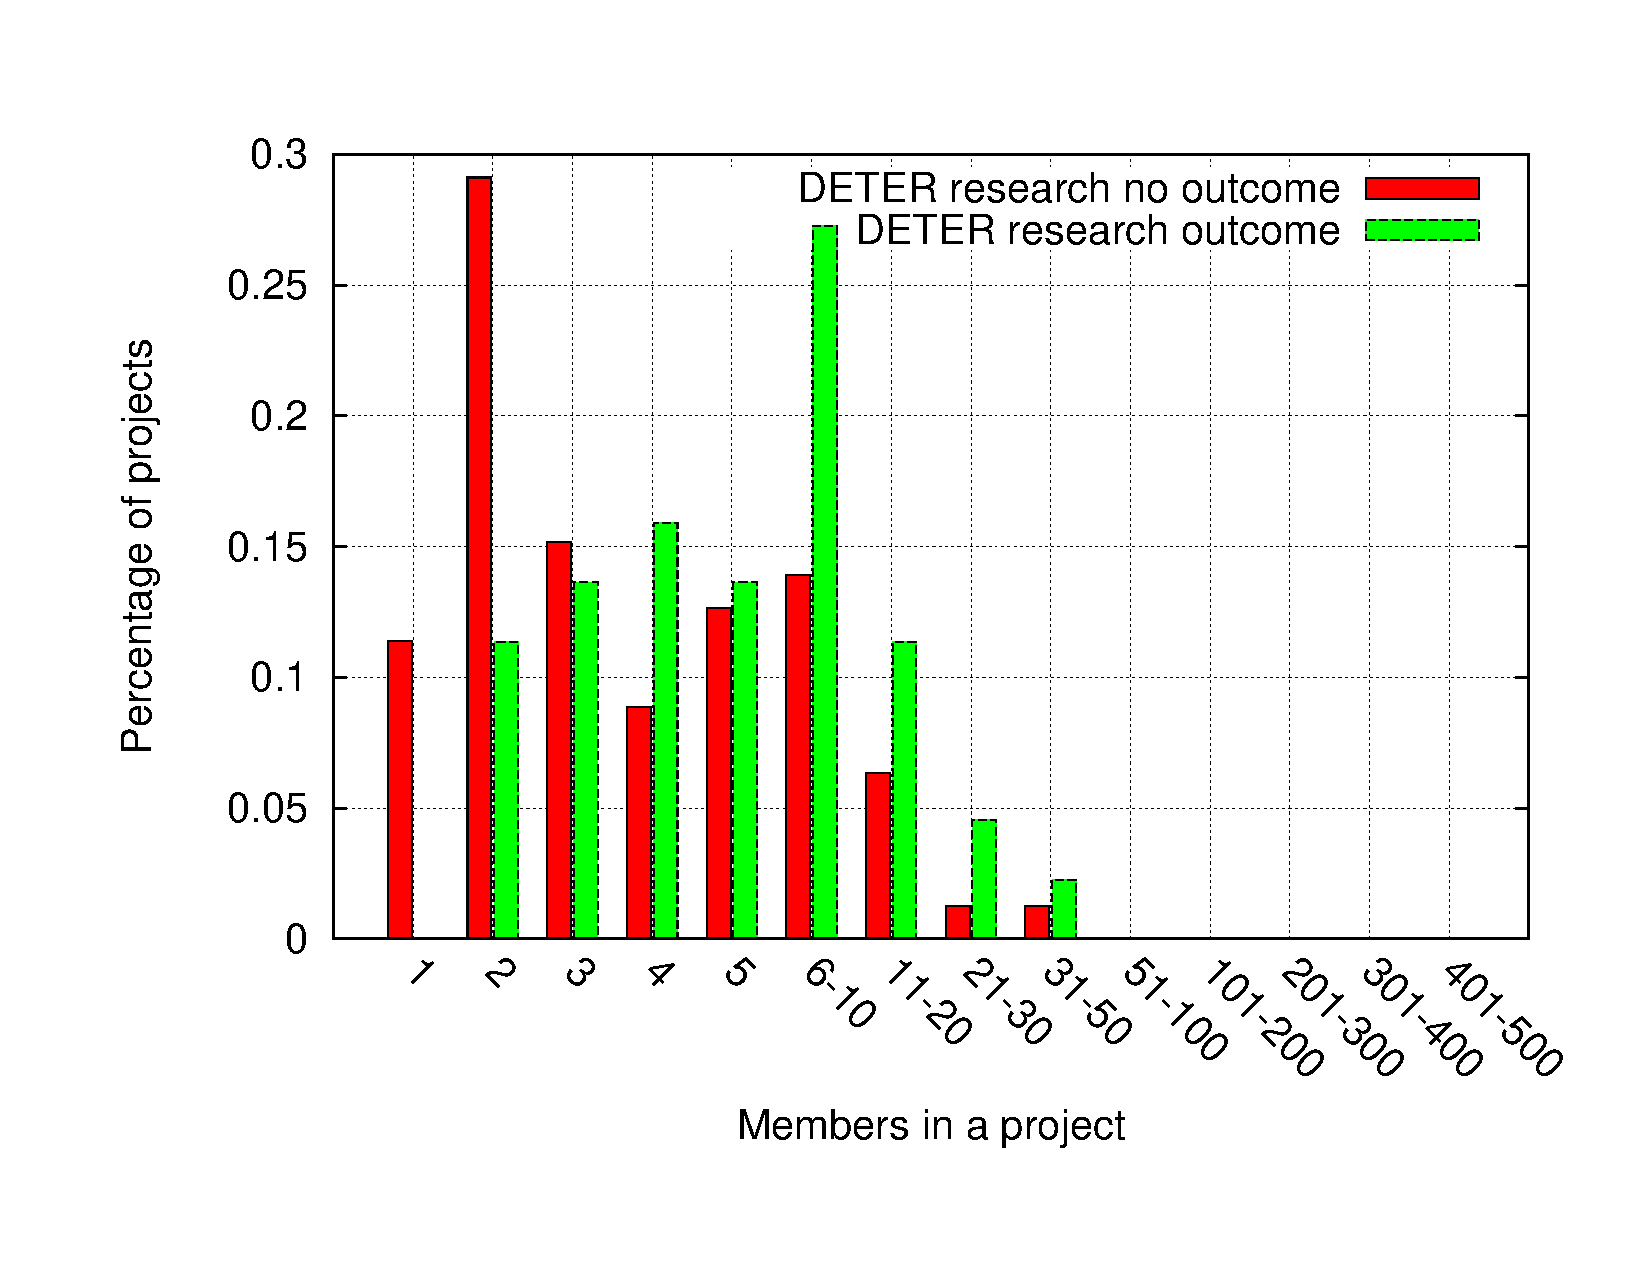
\includegraphics[width=3in,
type=pdf,ext=.pdf,read=.pdf]{figs/proj.user.cmp.gnu} \caption{Members
per project. Left: DETER vs Emulab, Right: All vs outcome}
\label{projuser} \end{center} \end{figure*}

\begin{figure*}[htbp] \begin{center} 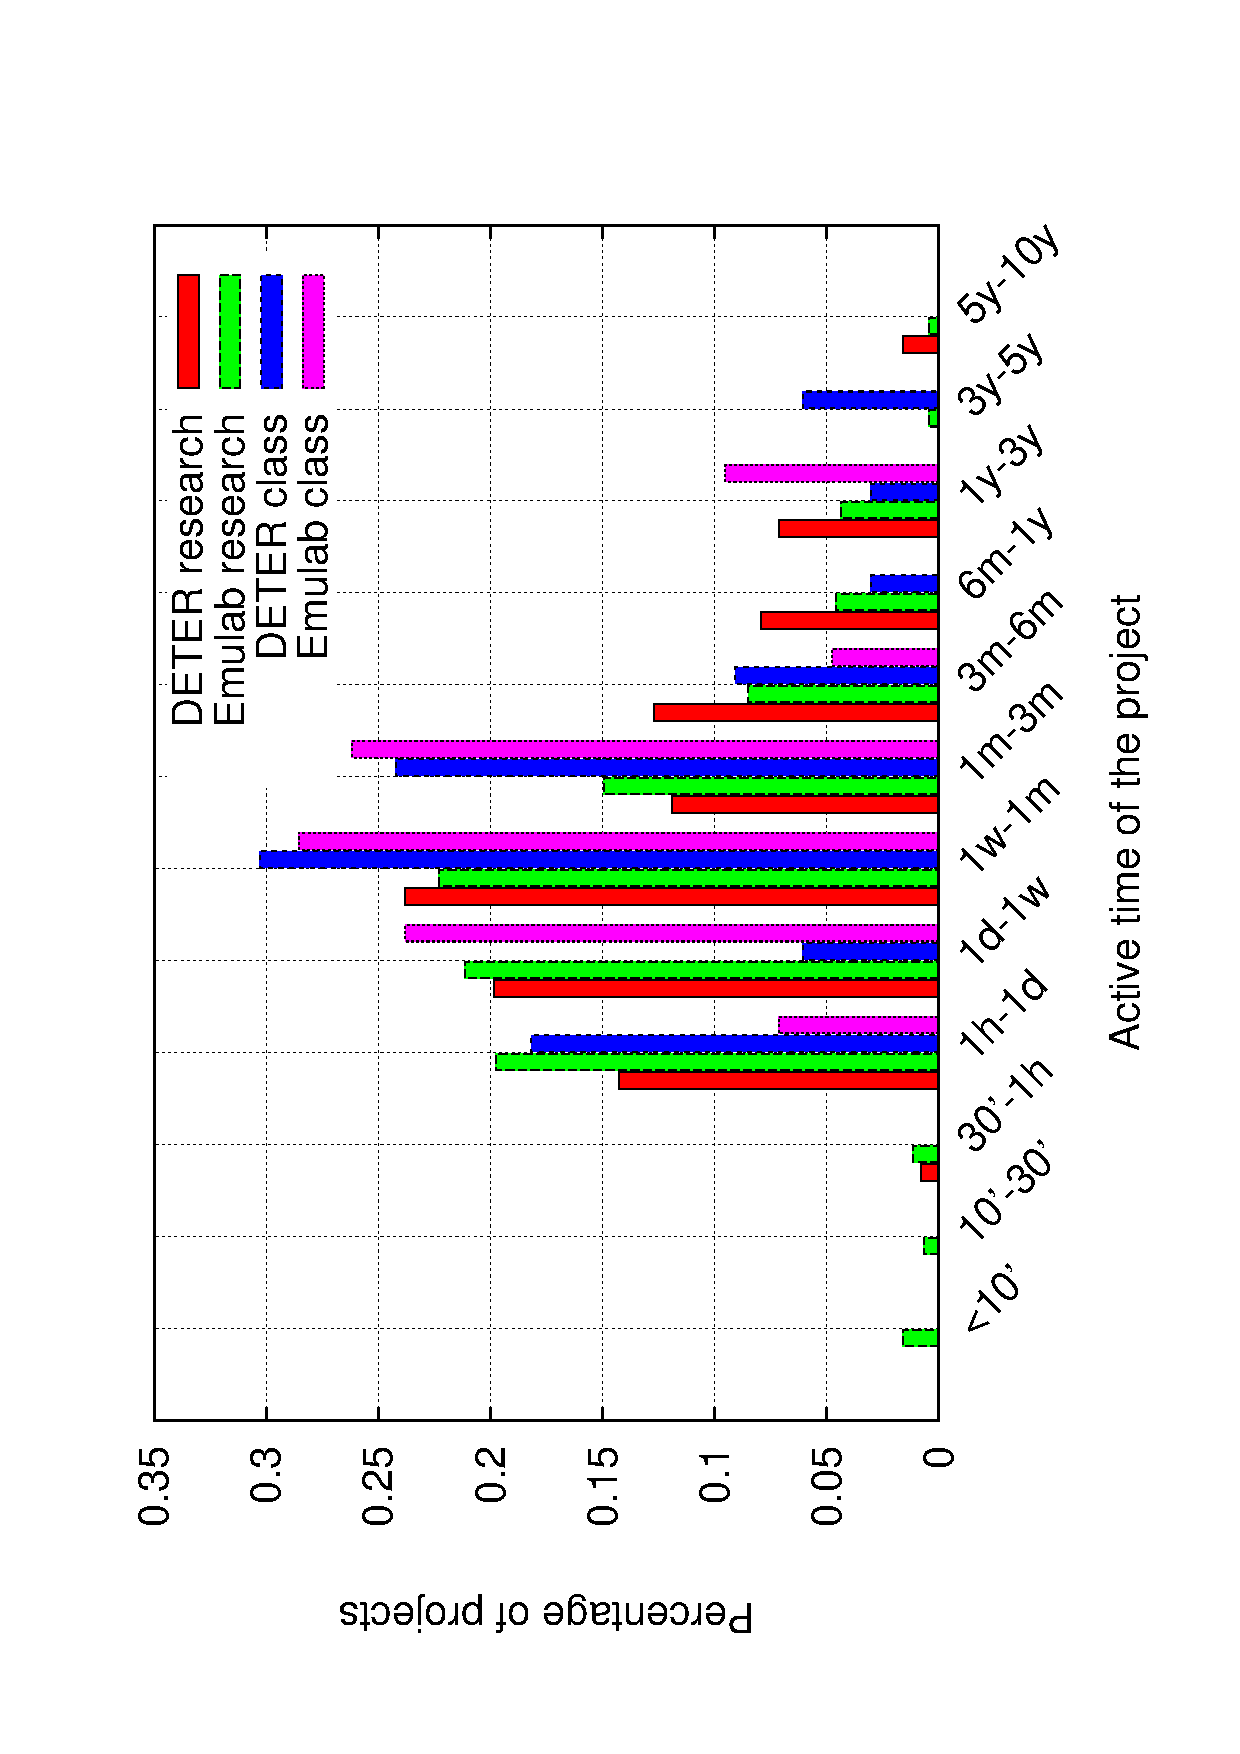
\includegraphics[width=3in,
type=pdf,ext=.pdf,read=.pdf]{figs/proj.active.gnu}
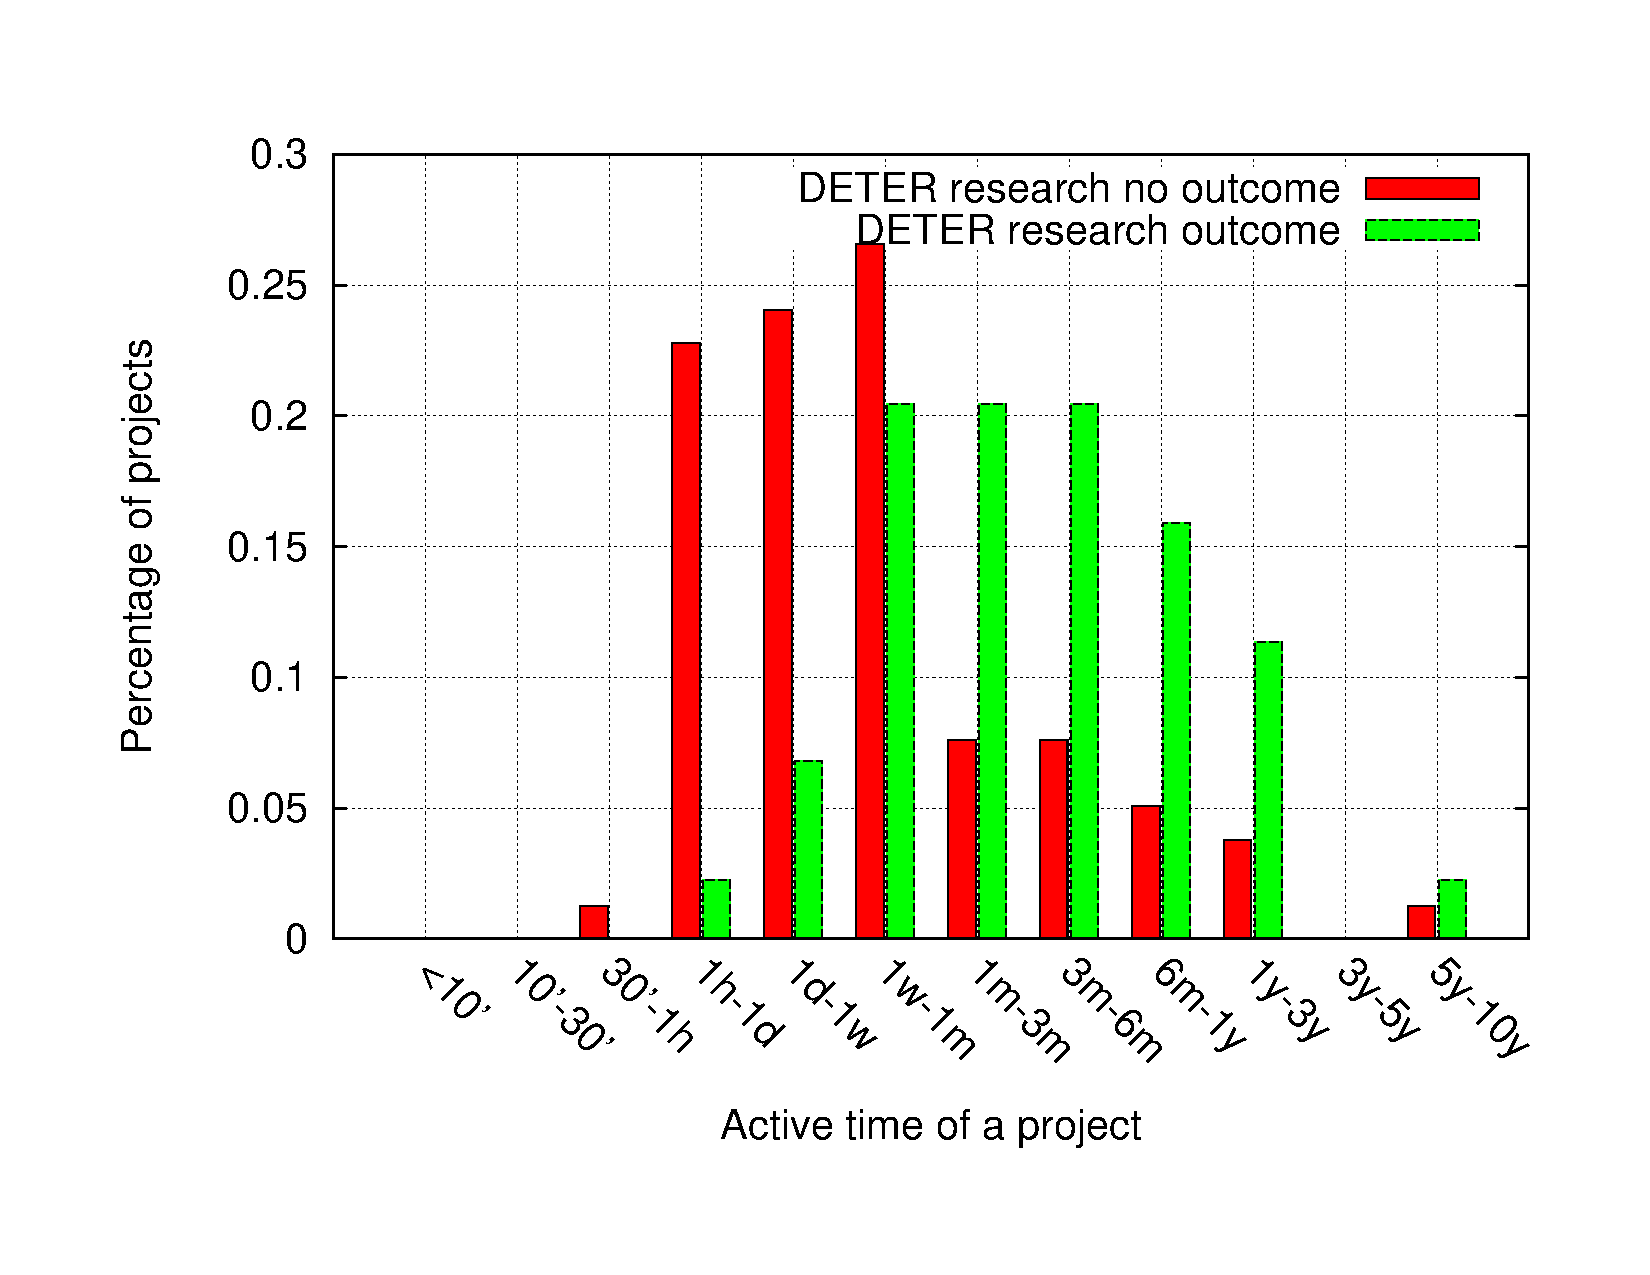
\includegraphics[width=3in,
type=pdf,ext=.pdf,read=.pdf]{figs/proj.active.cmp.gnu} \caption{Active
time of a project. Left: DETER vs Emulab, Right: All vs outcome}
\label{projactive} \end{center} \end{figure*}


\begin{figure*}[htbp] \begin{center} 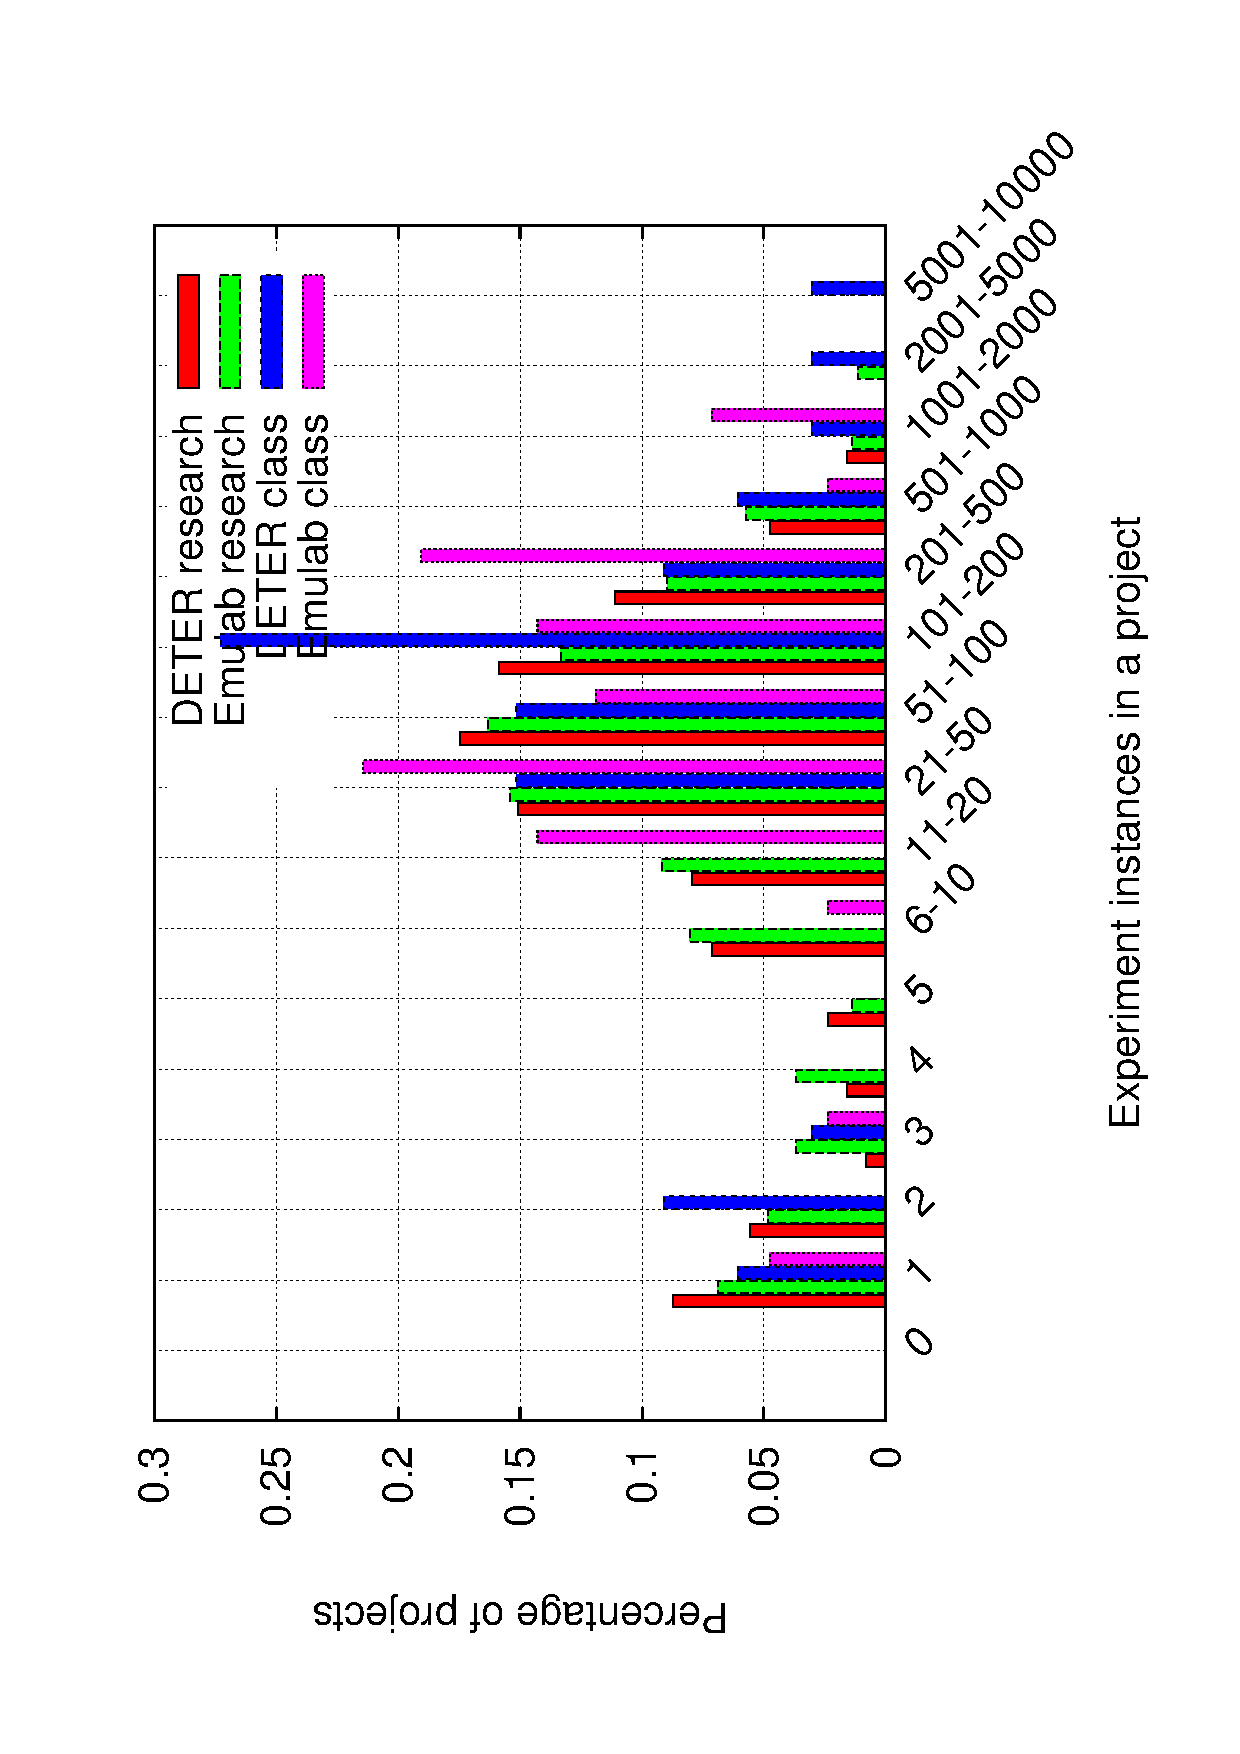
\includegraphics[width=3in,
type=pdf,ext=.pdf,read=.pdf]{figs/proj.swaps.gnu}
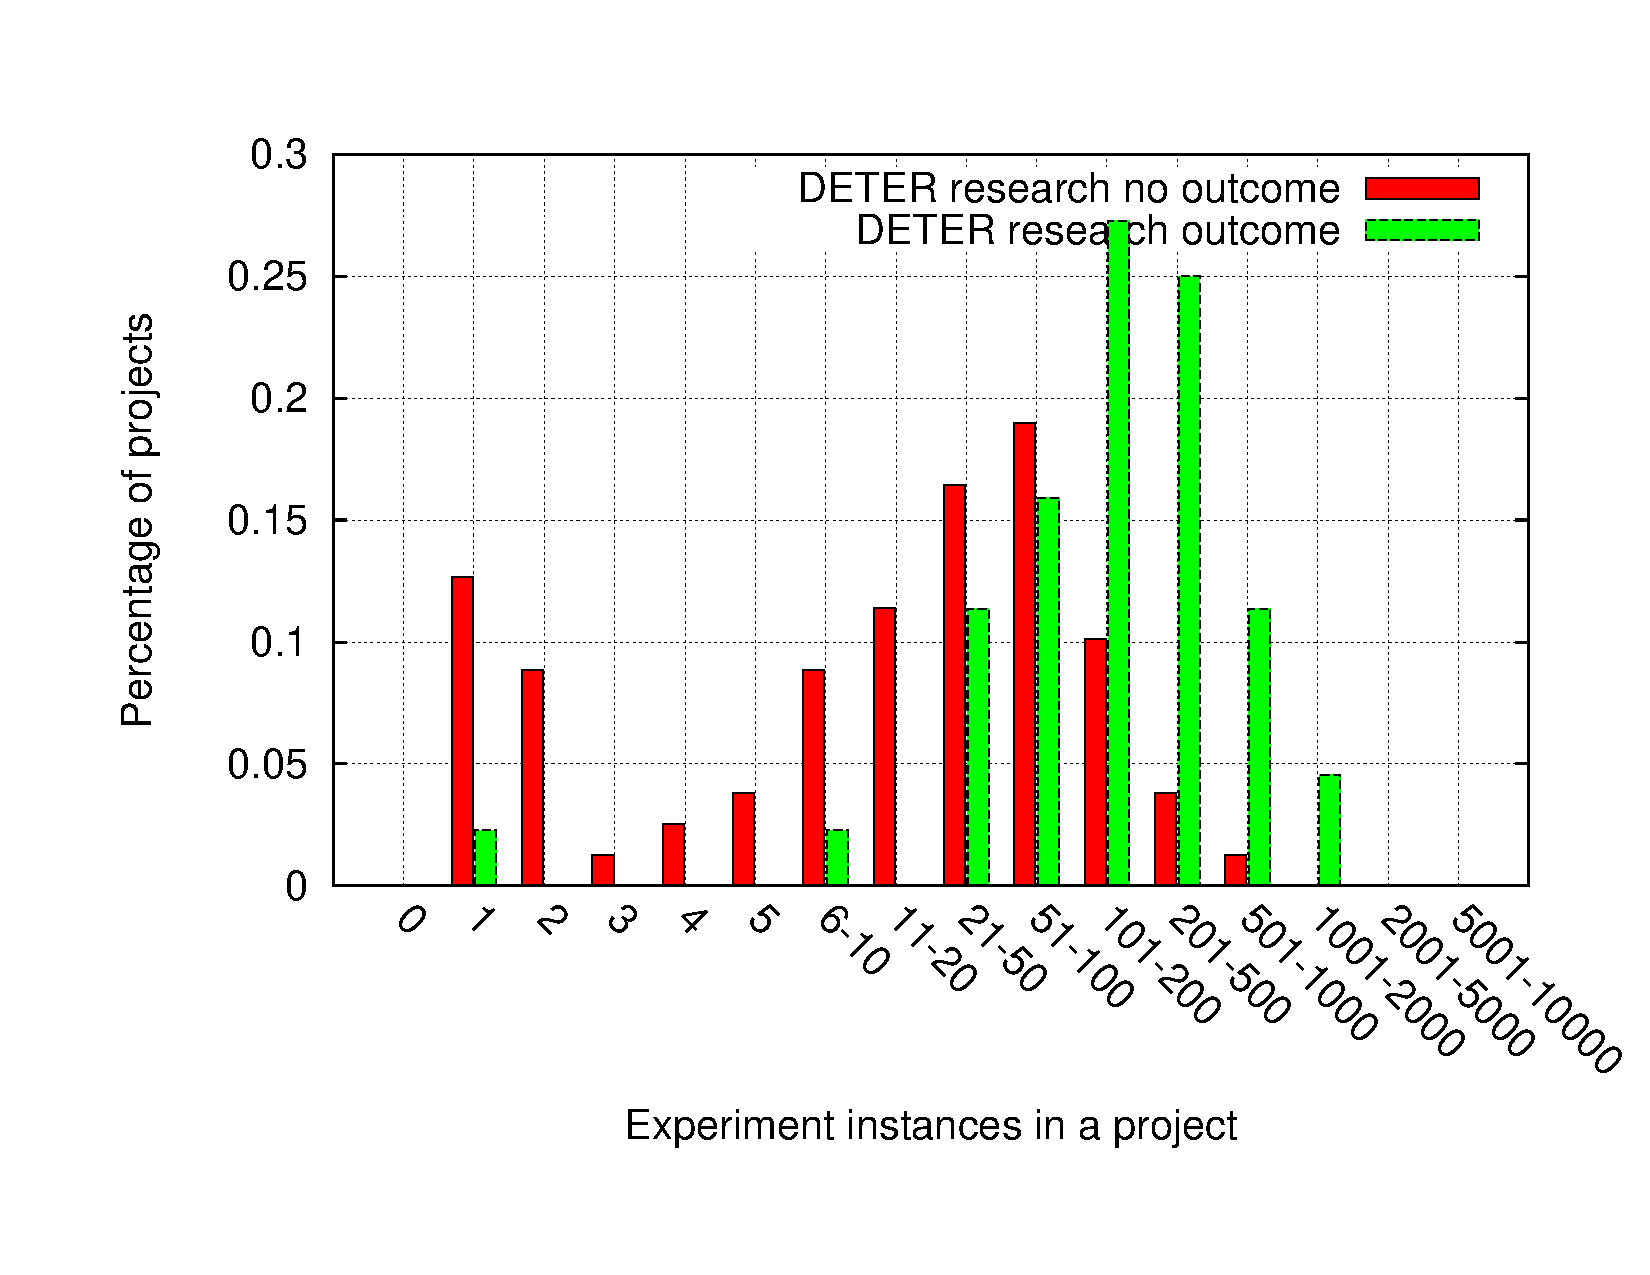
\includegraphics[width=3in,
type=pdf,ext=.pdf,read=.pdf]{figs/proj.swaps.cmp.gnu}
\caption{Experiment instances in a project. Left: DETER vs Emulab,
Right: All vs outcome} \label{projswaps} \end{center} \end{figure*}

Are outcome projects more active because they have been around longer or
because they work harder? Both. Figure \ref{projagevsactive} shows that.
Figure \ref{projuservsauser} shows that in large research projects with
outcome almost all users are active, while in smaller projects only a
few may be active. What's surprising is that for classes with outcome
sometimes only half of the users are active. This may be due to them
having a choice of using DETER vs not or maybe because we create more
accounts than needed for the class.

\begin{figure*}[htbp] \begin{center} 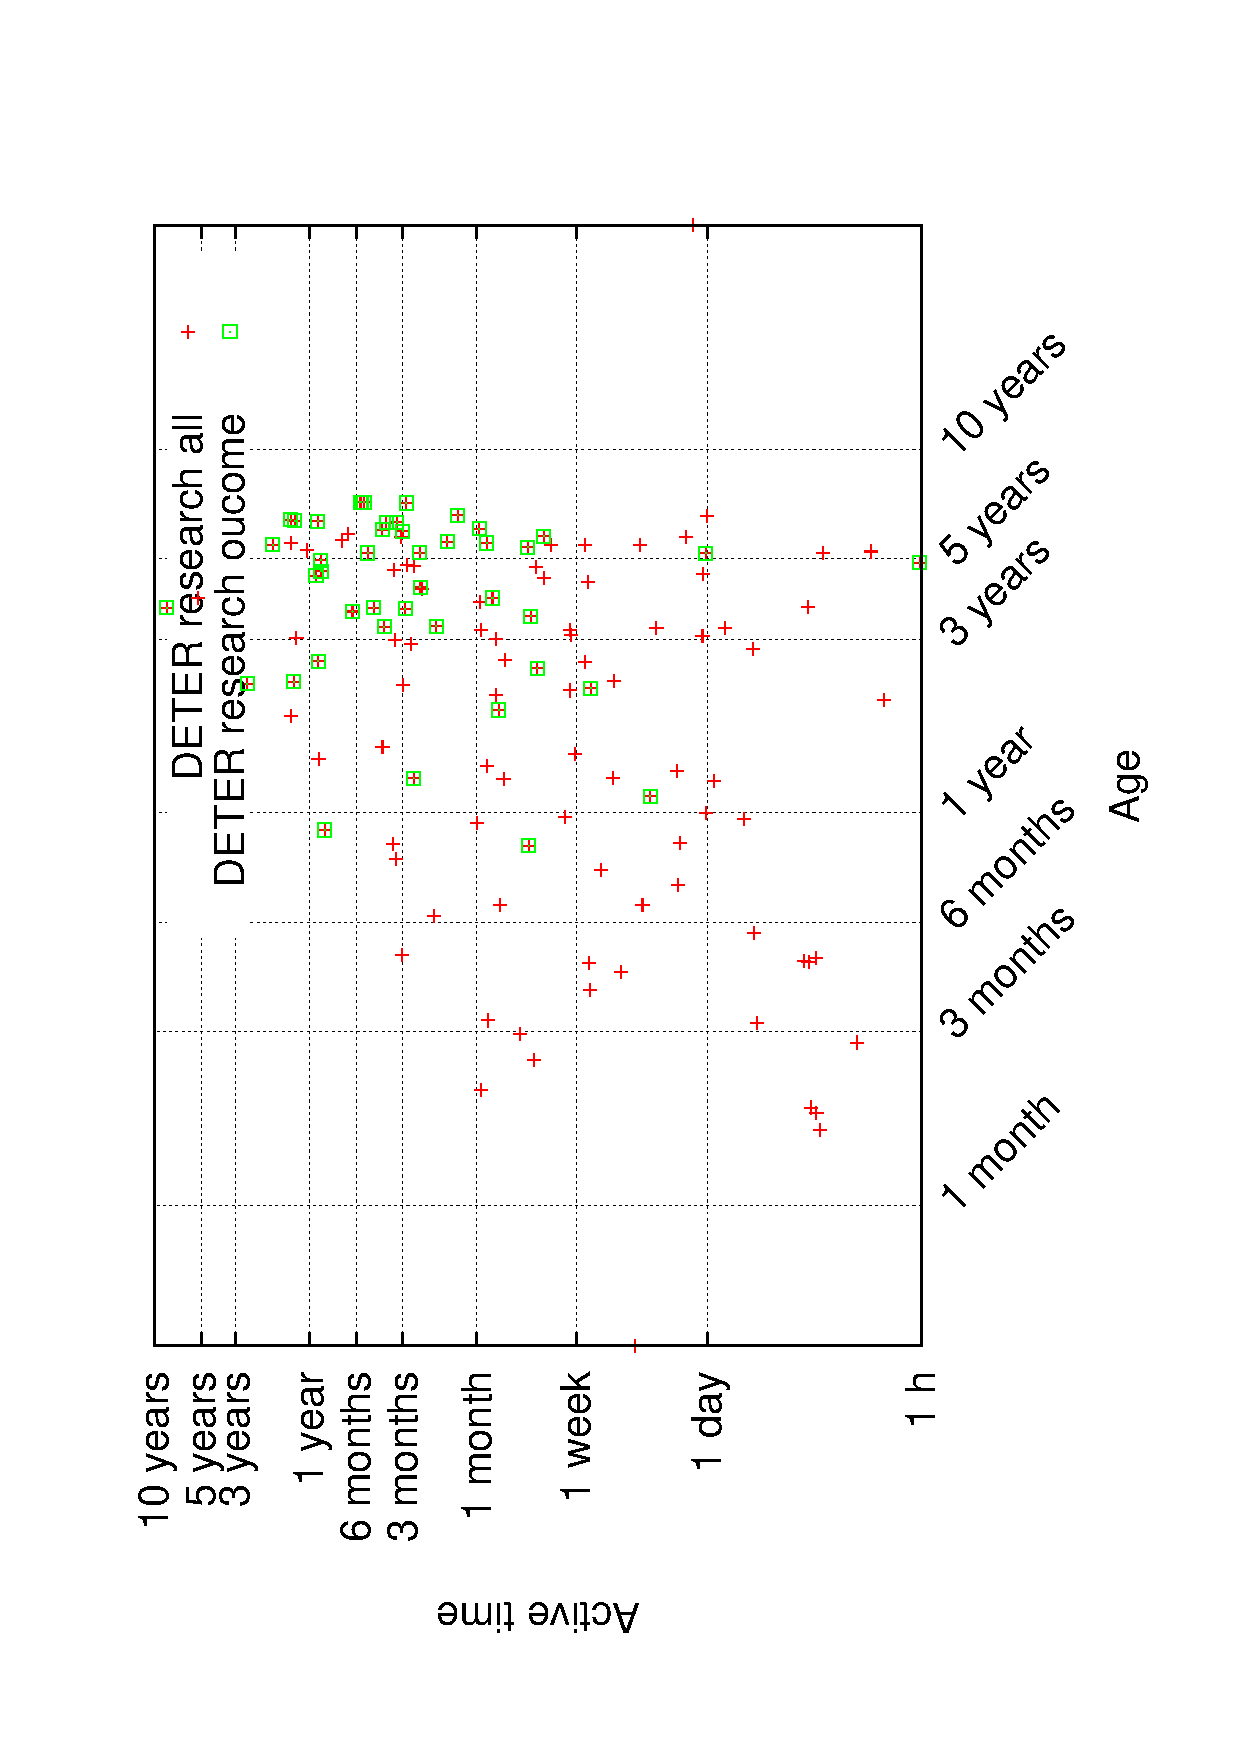
\includegraphics[width=3in,
type=pdf,ext=.pdf,read=.pdf]{figs/proj.agevsactive.res.gnu}
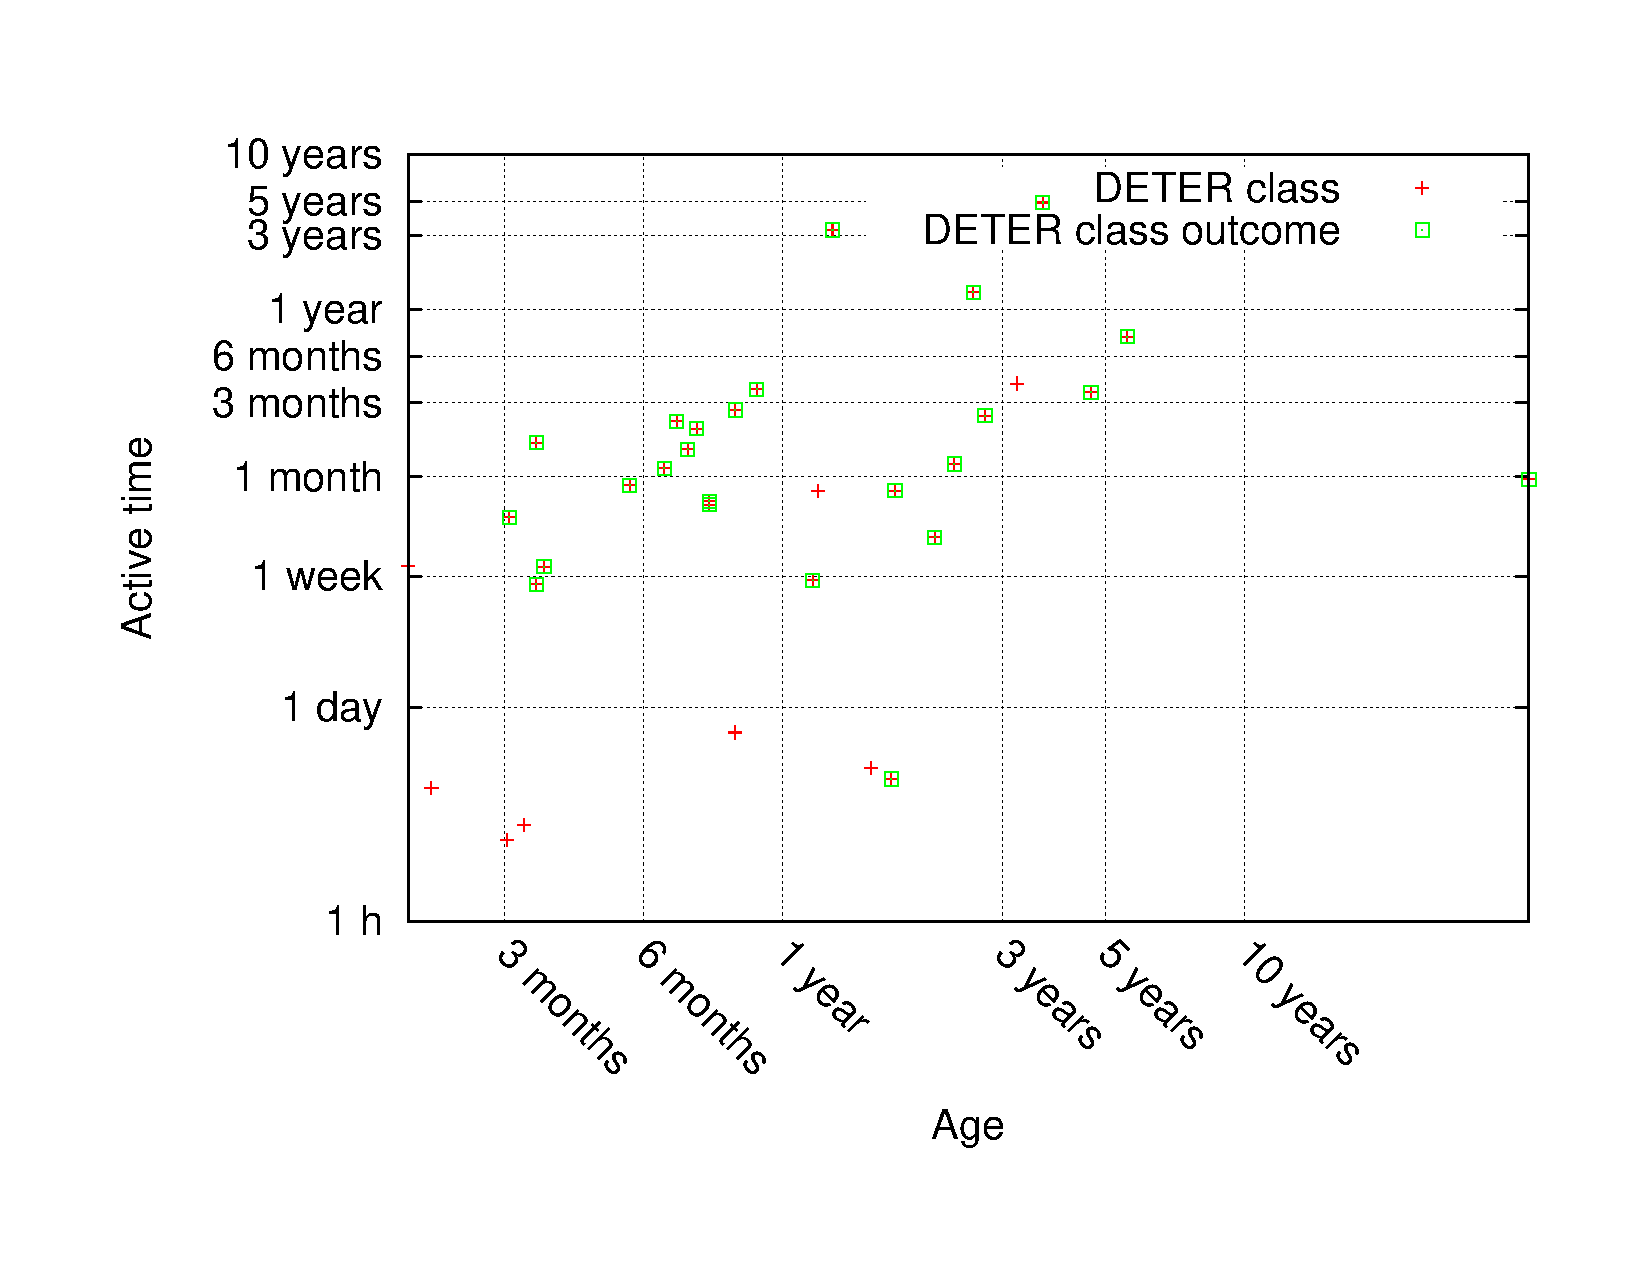
\includegraphics[width=3in,
type=pdf,ext=.pdf,read=.pdf]{figs/proj.agevsactivecl.gnu}
\caption{Active time vs age of a project. Left: DETER research, right:
DETER class} \label{projagevsactive} \end{center} \end{figure*}

\begin{figure*}[htbp] \begin{center} 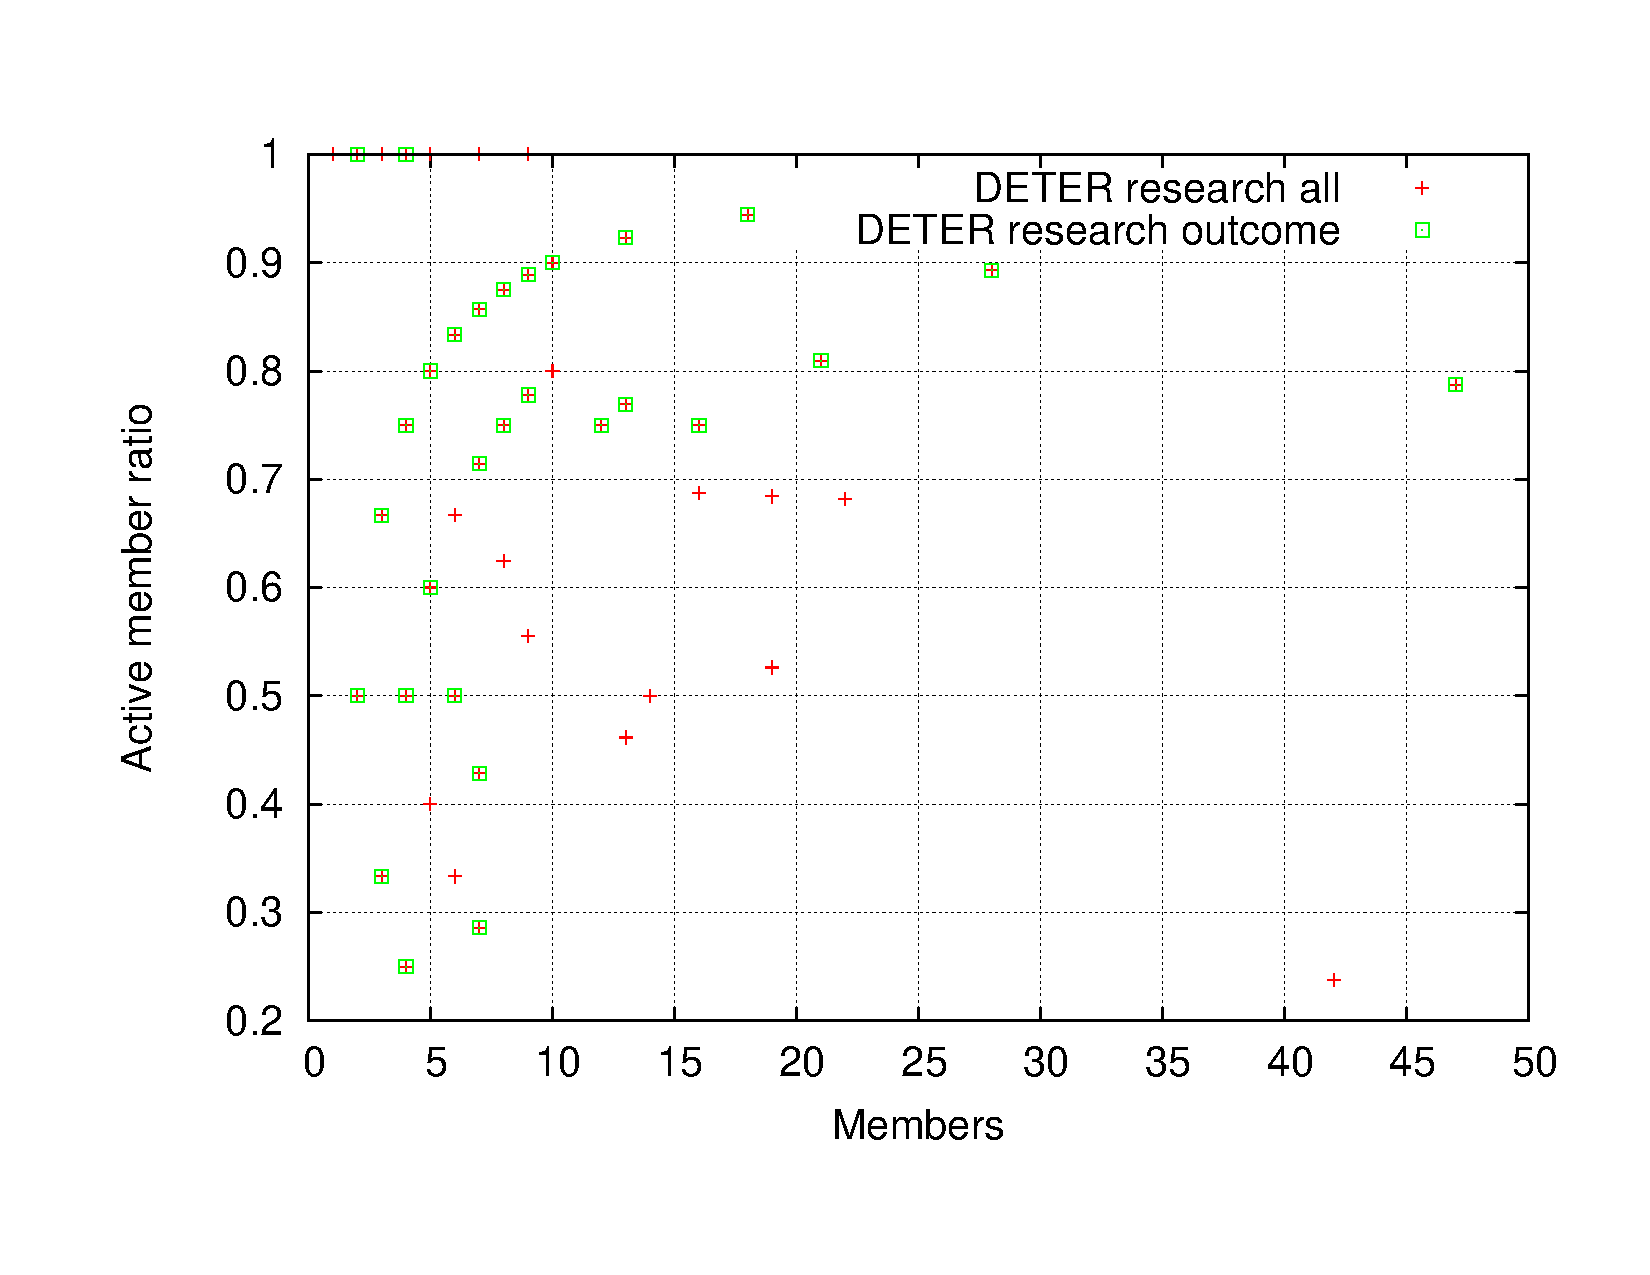
\includegraphics[width=3in,
type=pdf,ext=.pdf,read=.pdf]{figs/proj.uservsauserres.gnu}
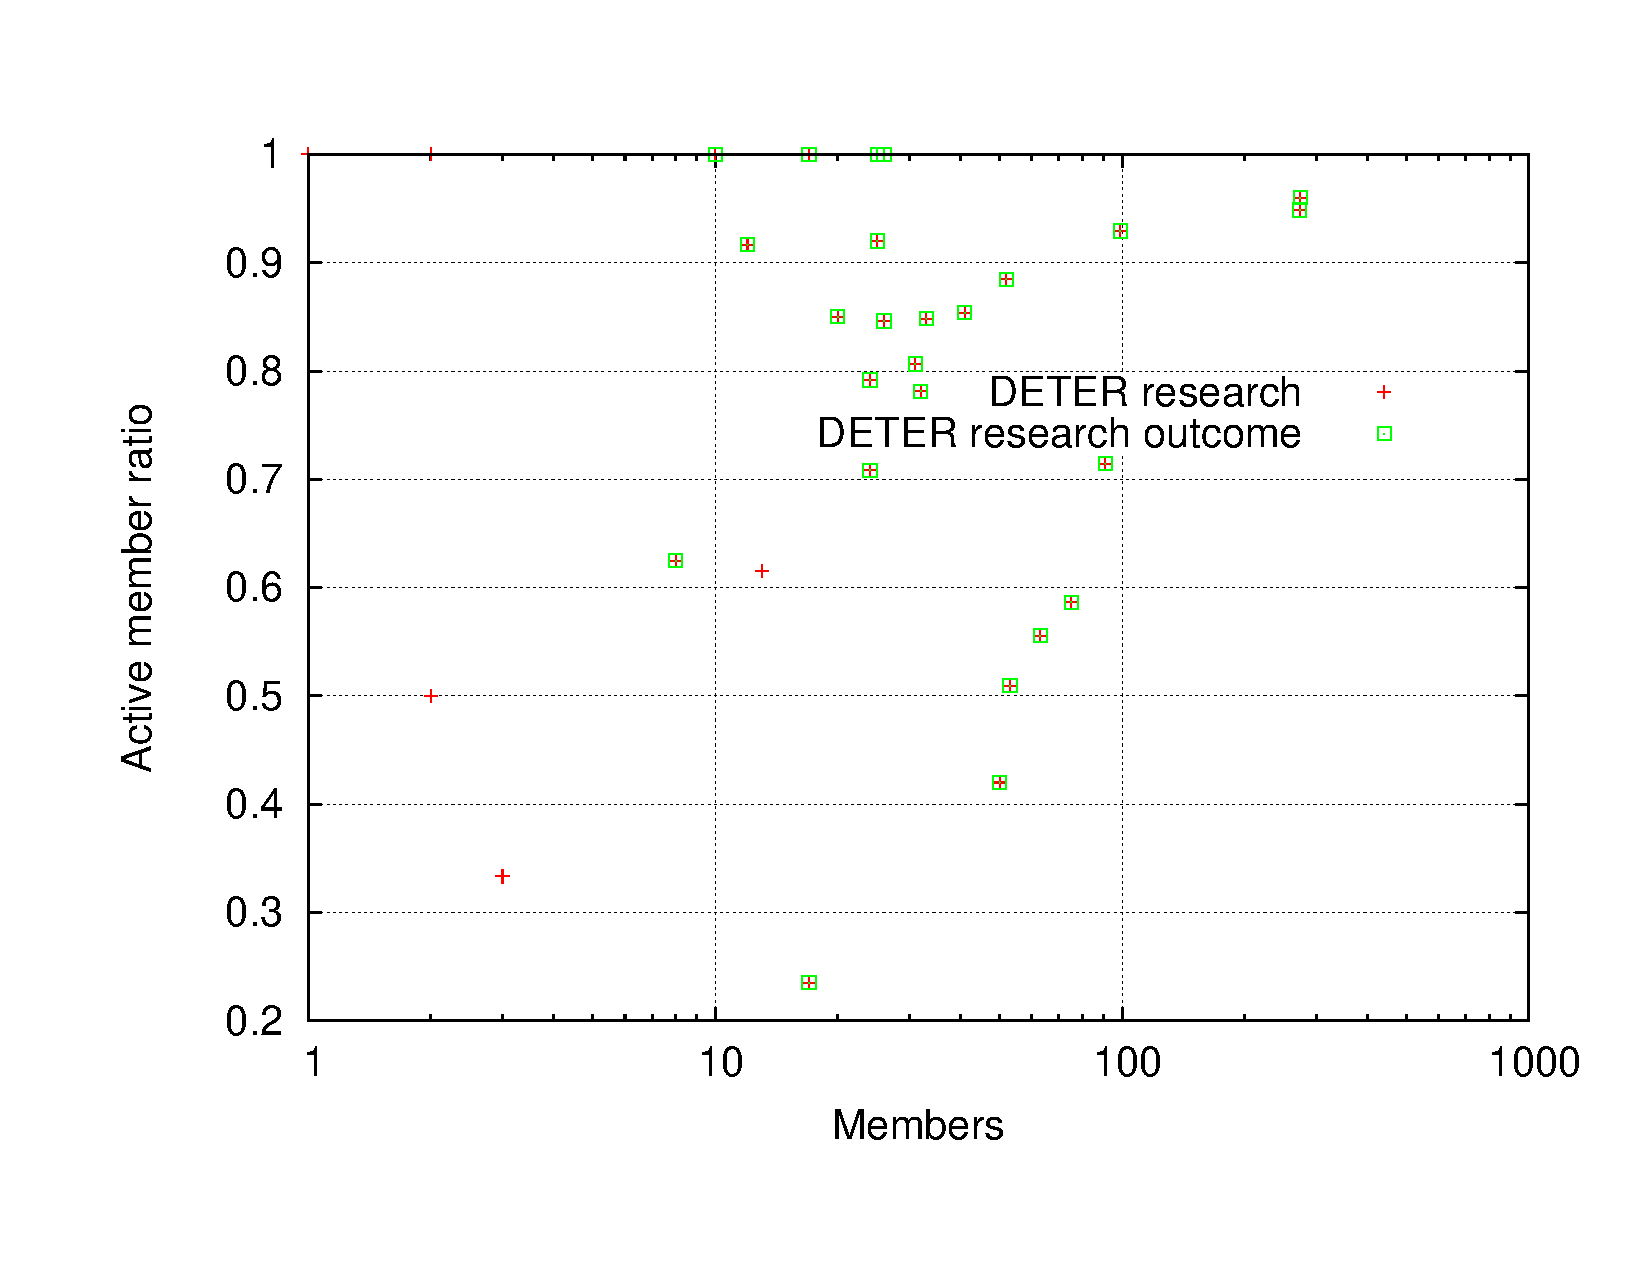
\includegraphics[width=3in,
type=pdf,ext=.pdf,read=.pdf]{figs/proj.uservsausercl.gnu}
\caption{Active member ratio vs all members of a project. Left: DETER
research, right: DETER class} \label{projuservsauser} \end{center}
\end{figure*}

Explain project evolution from inception to publication. Quantify how
many projects do not result in productive use. Some don't manipulate
experiments at all. Some are idle. Quantify this for users as well.
Quantify this for experiments and for idleness as well. Not sure if
idleness goes here.


\section{User Patterns}

\begin{figure*}[htbp] \begin{center} 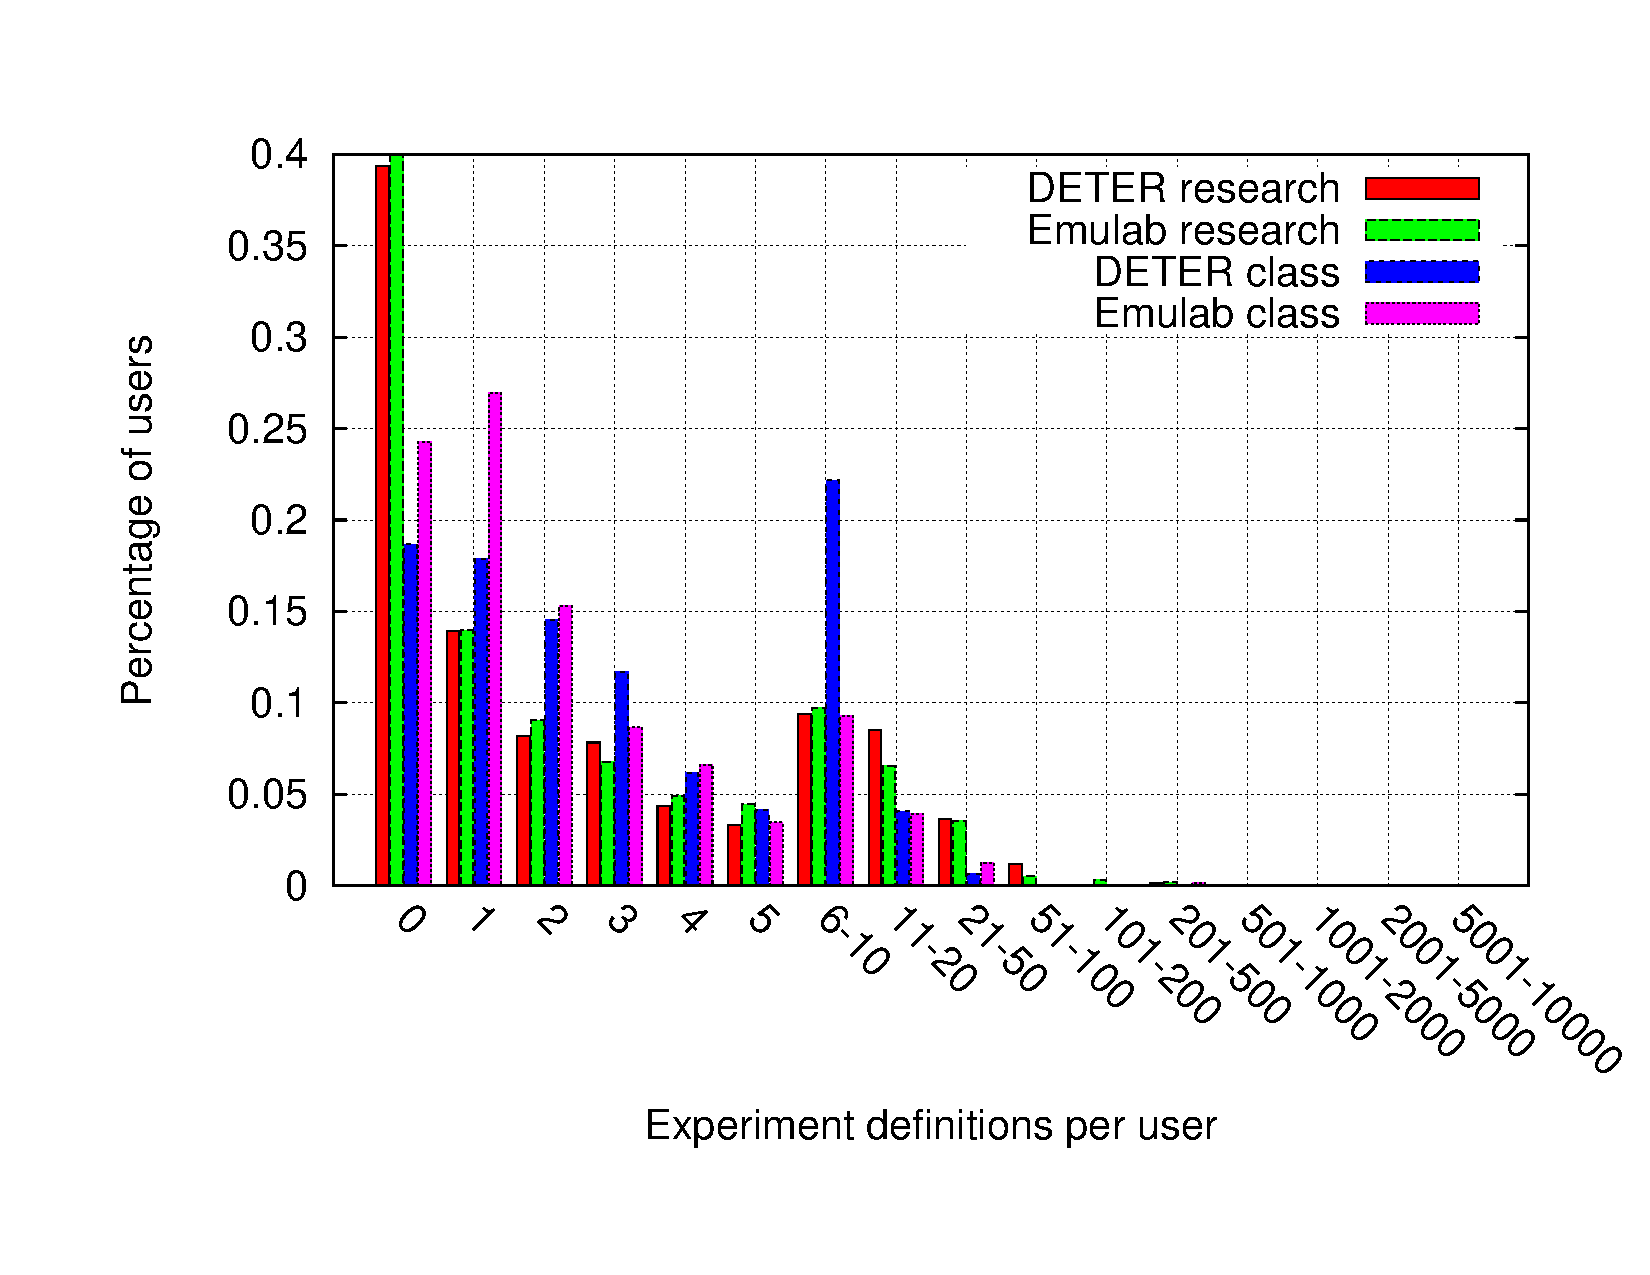
\includegraphics[width=3in,
type=pdf,ext=.pdf,read=.pdf]{figs/user.exp.gnu}
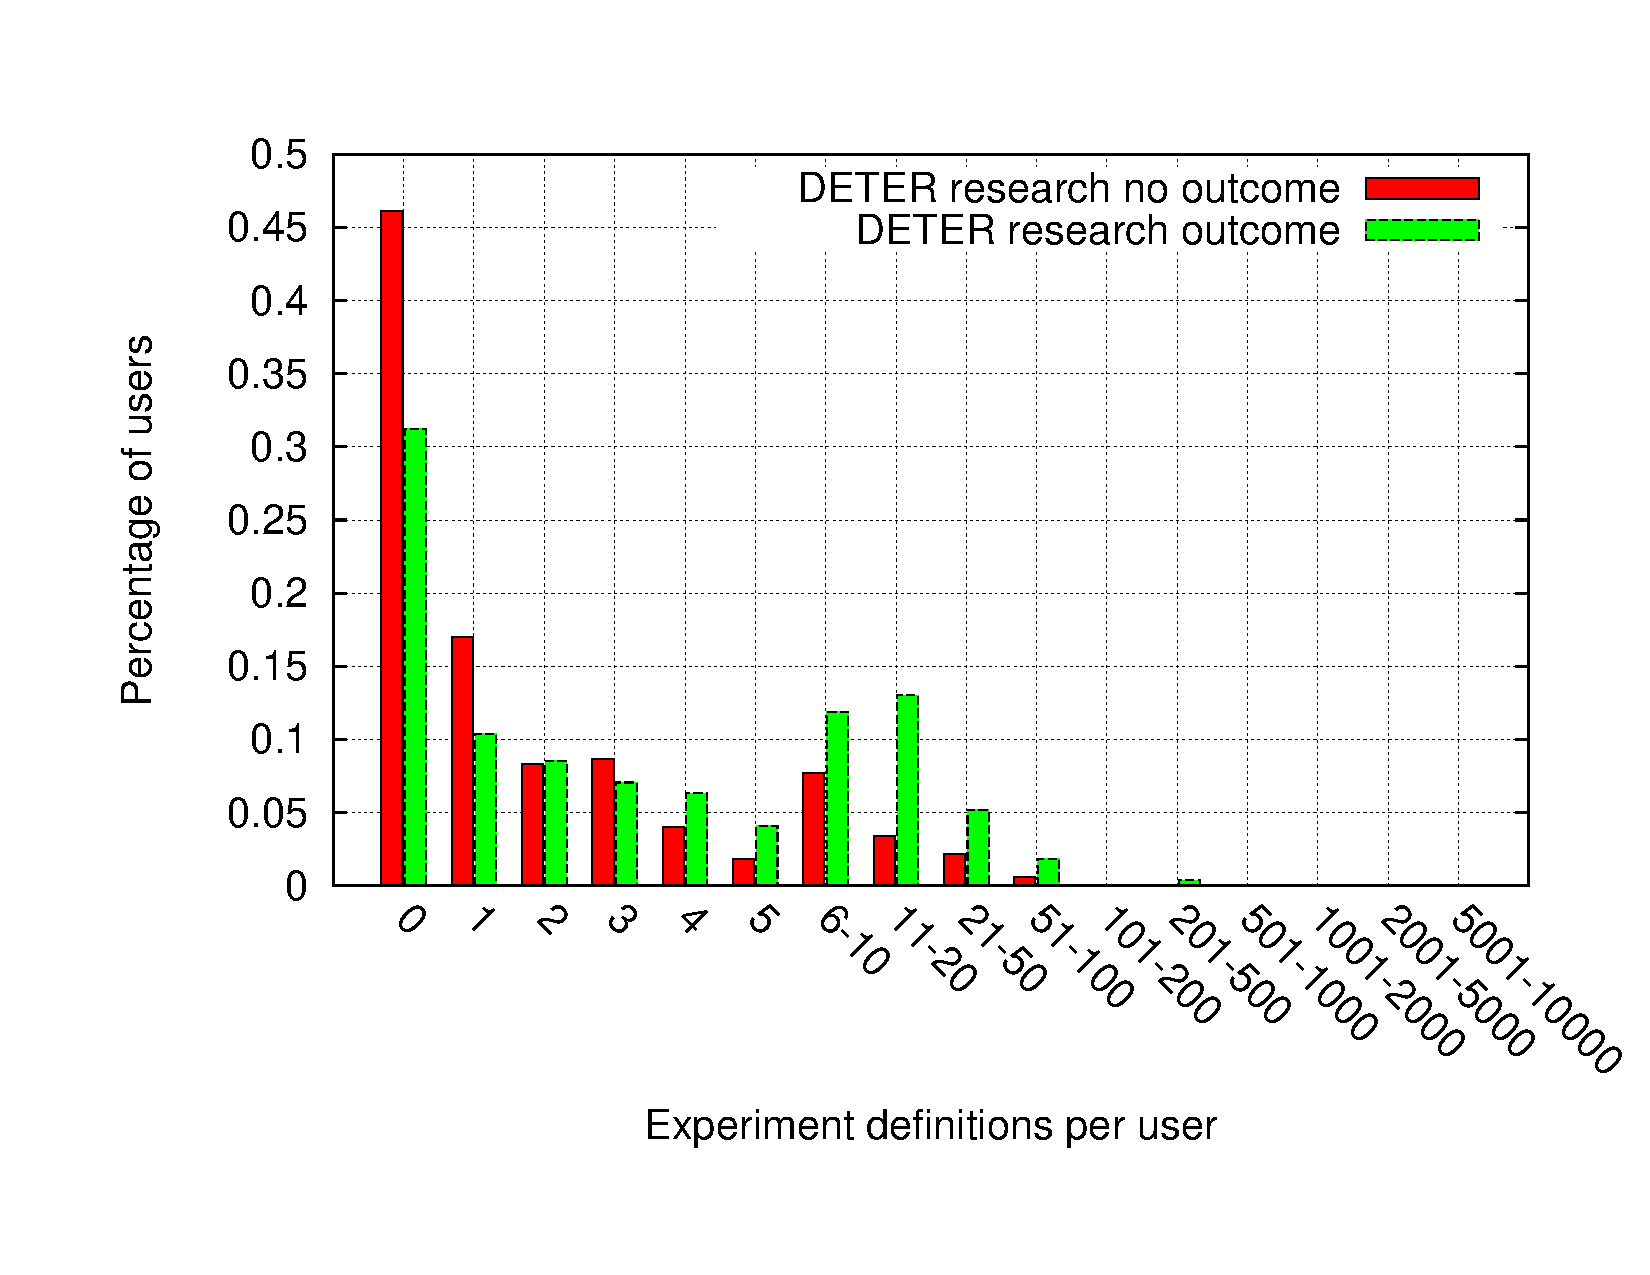
\includegraphics[width=3in,
type=pdf,ext=.pdf,read=.pdf]{figs/user.exp.cmp.gnu} \caption{Experiment
definitions per user. Left: DETER vs Emulab, Right: All vs outcome}
\label{userexp} \end{center} \end{figure*}

\begin{figure*}[htbp] \begin{center} 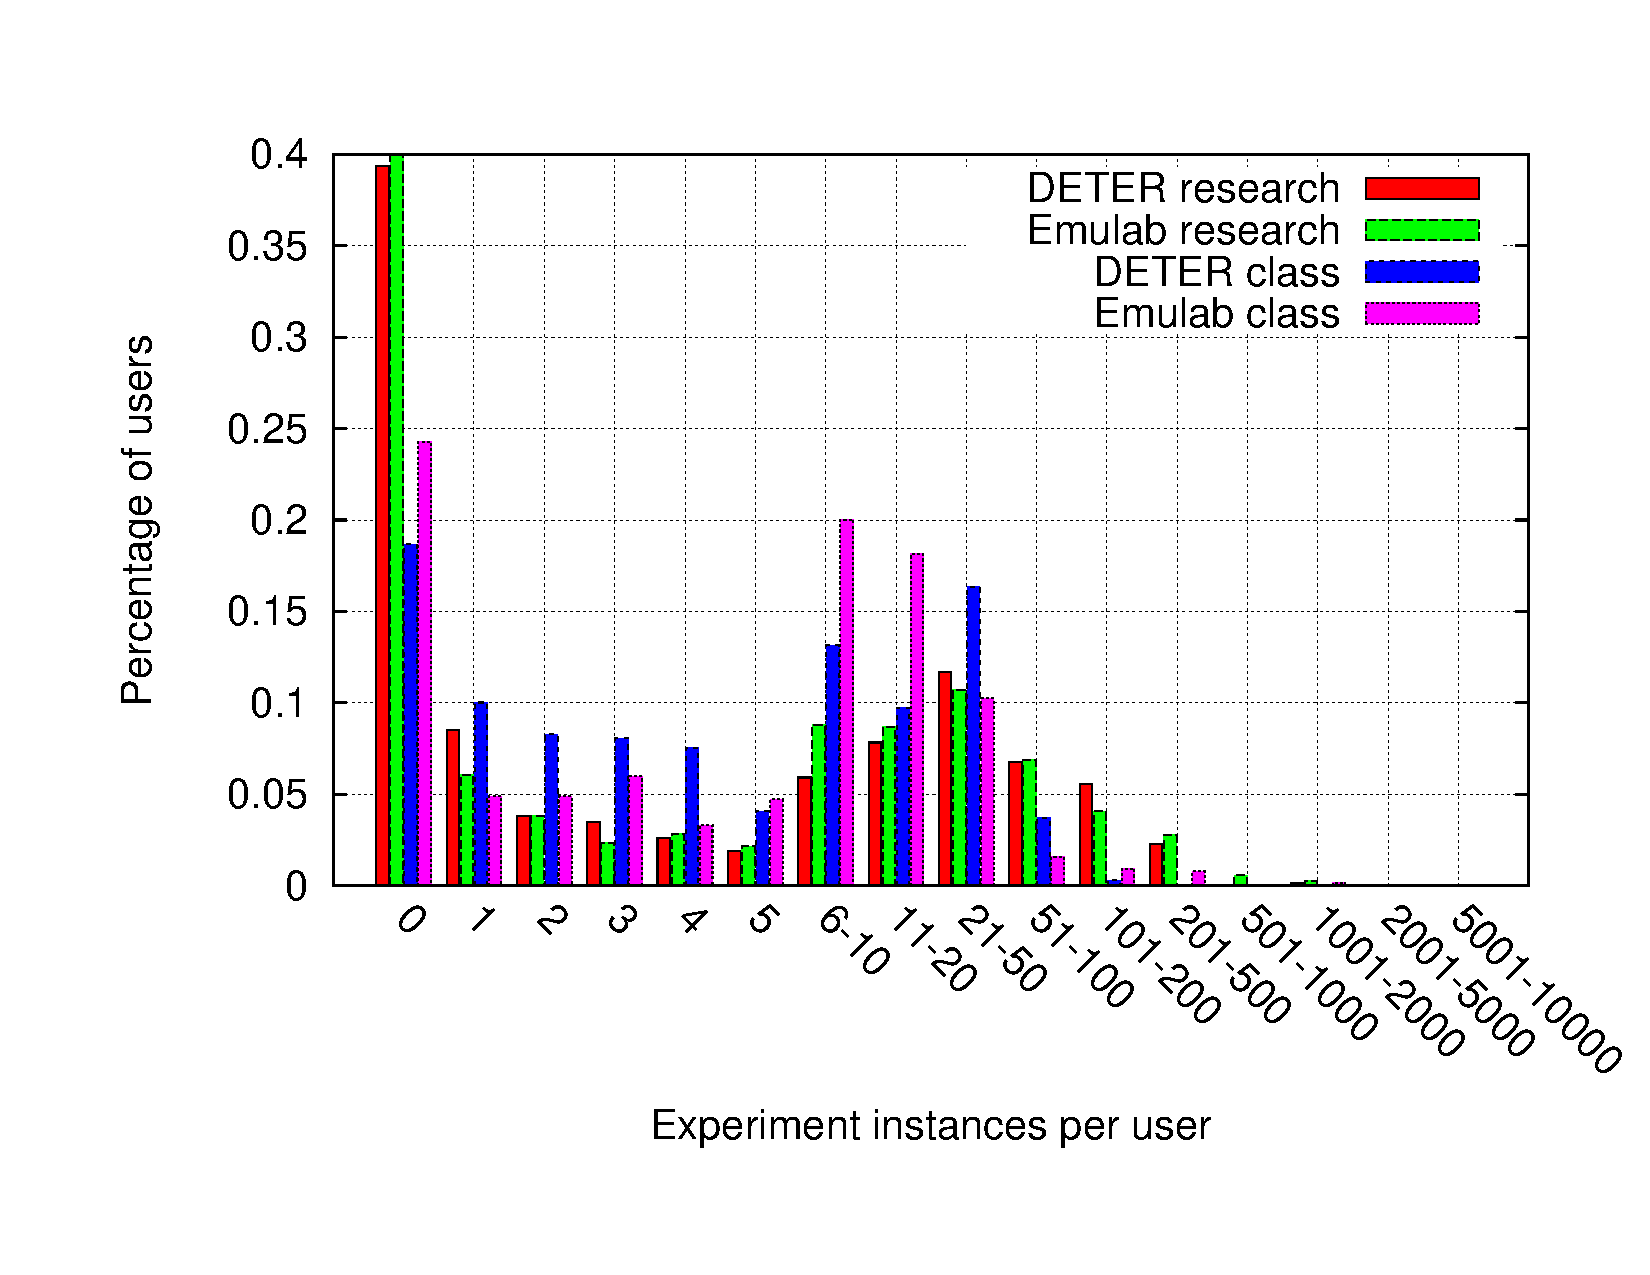
\includegraphics[width=3in,
type=pdf,ext=.pdf,read=.pdf]{figs/user.swaps.gnu}
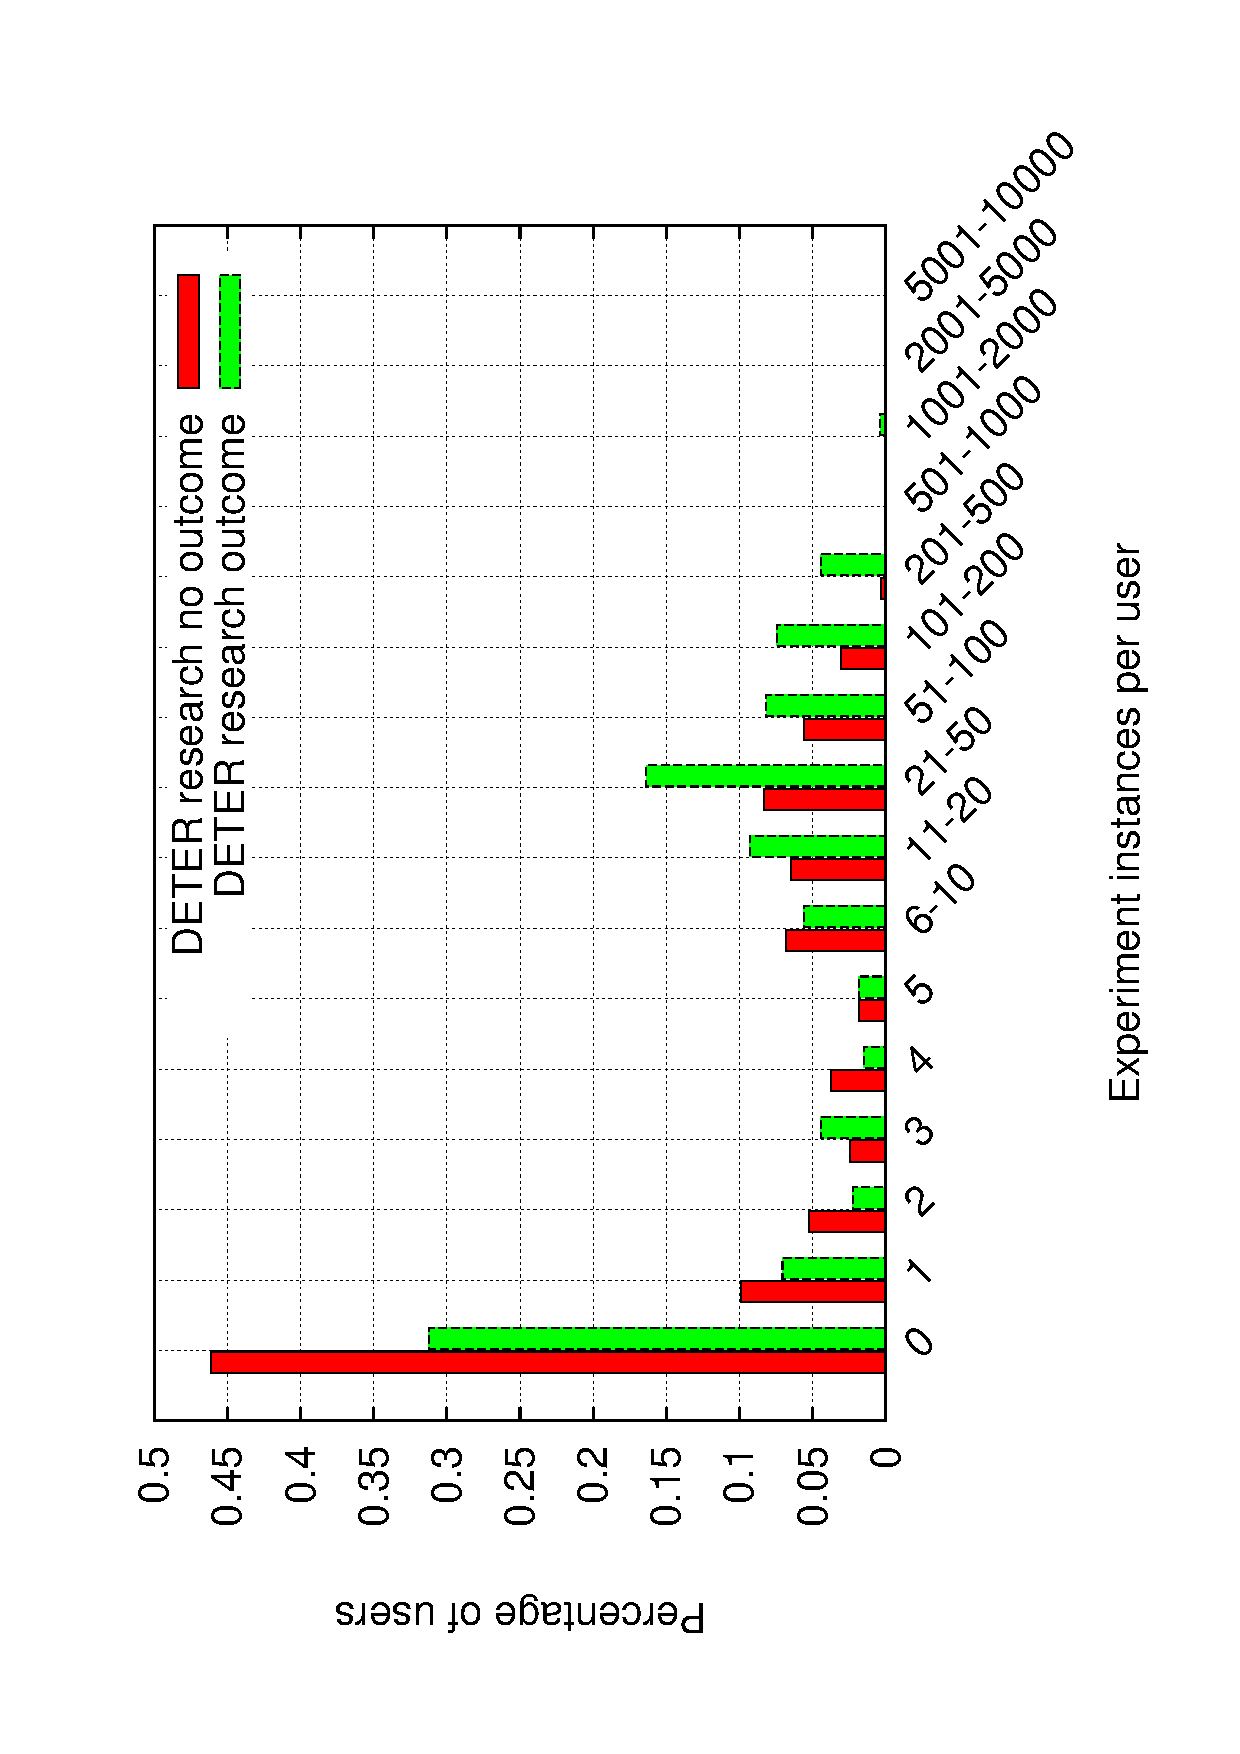
\includegraphics[width=3in,
type=pdf,ext=.pdf,read=.pdf]{figs/user.swaps.cmp.gnu}
\caption{Experiment instances per user. Left: DETER vs Emulab, Right:
All vs outcome} \label{userswaps} \end{center} \end{figure*}

\begin{figure*}[htbp] \begin{center} 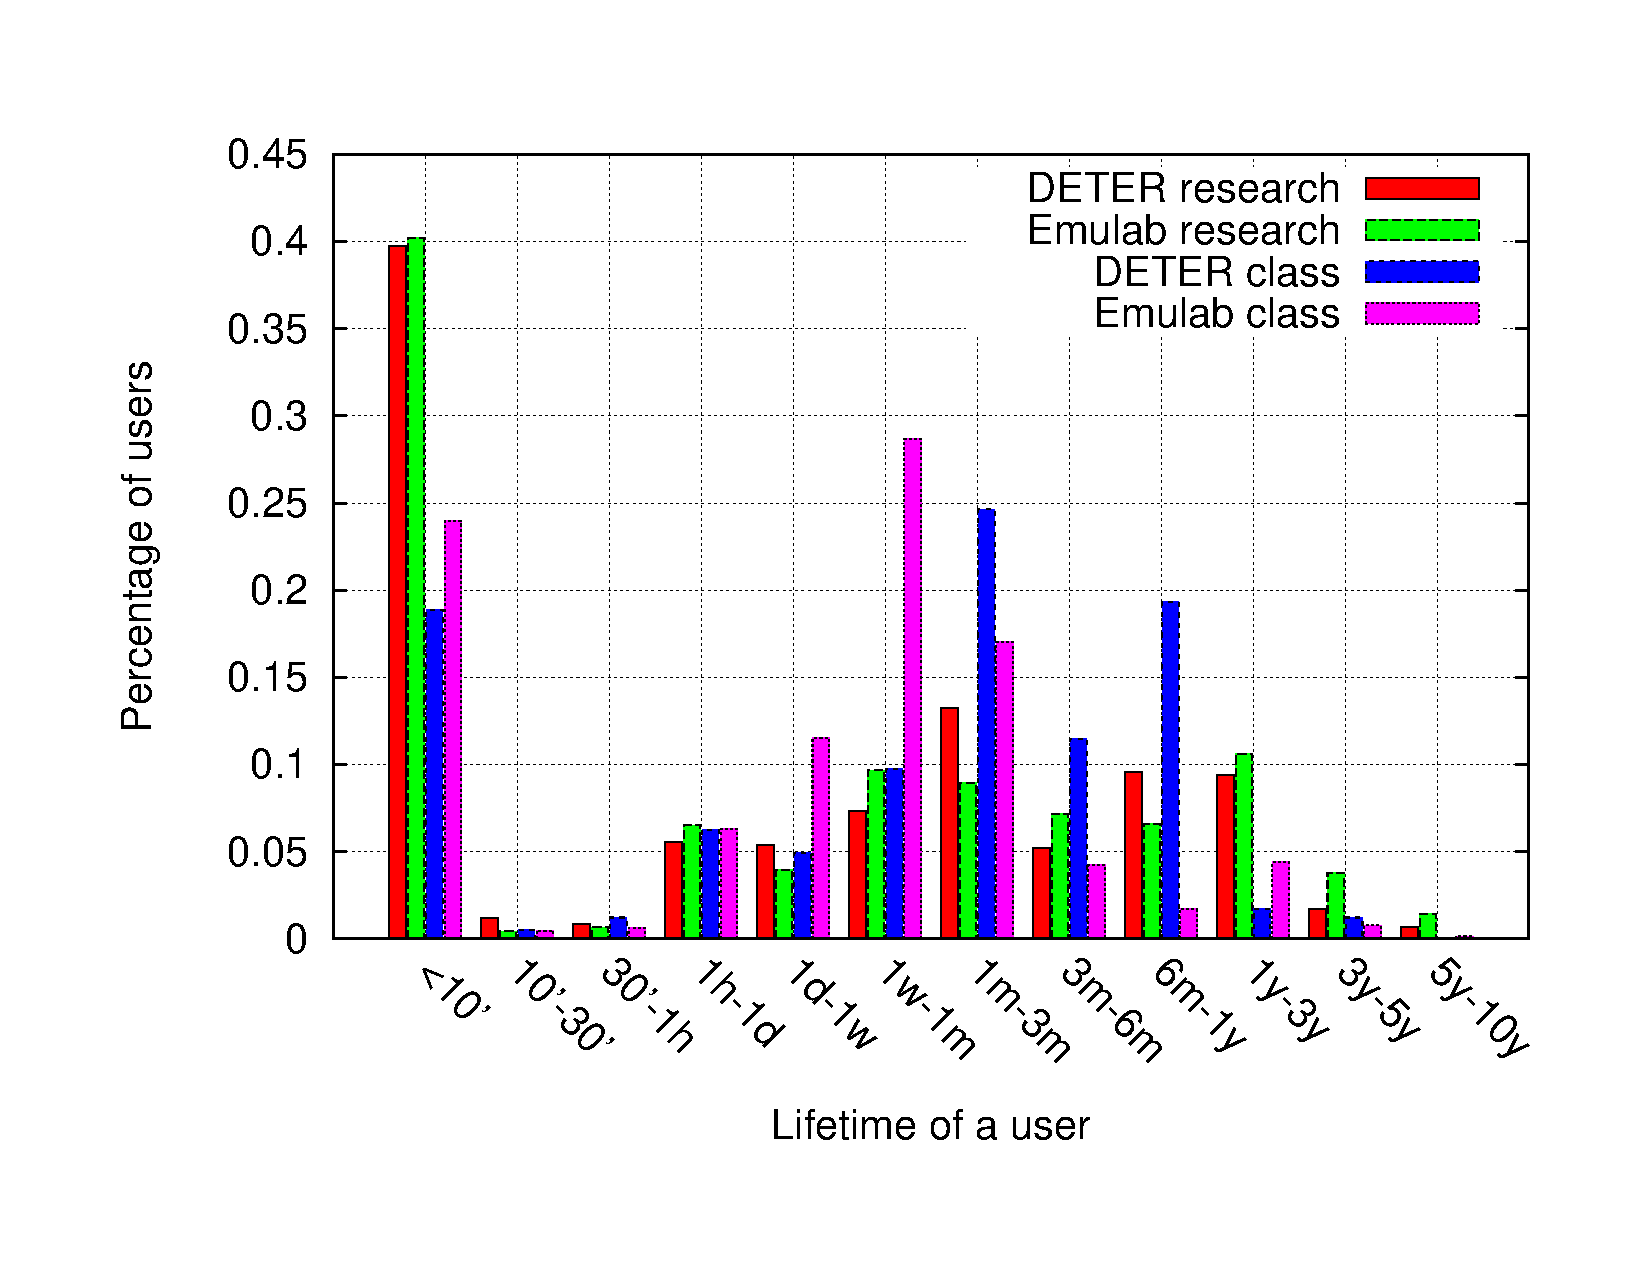
\includegraphics[width=3in,
type=pdf,ext=.pdf,read=.pdf]{figs/user.life.gnu}
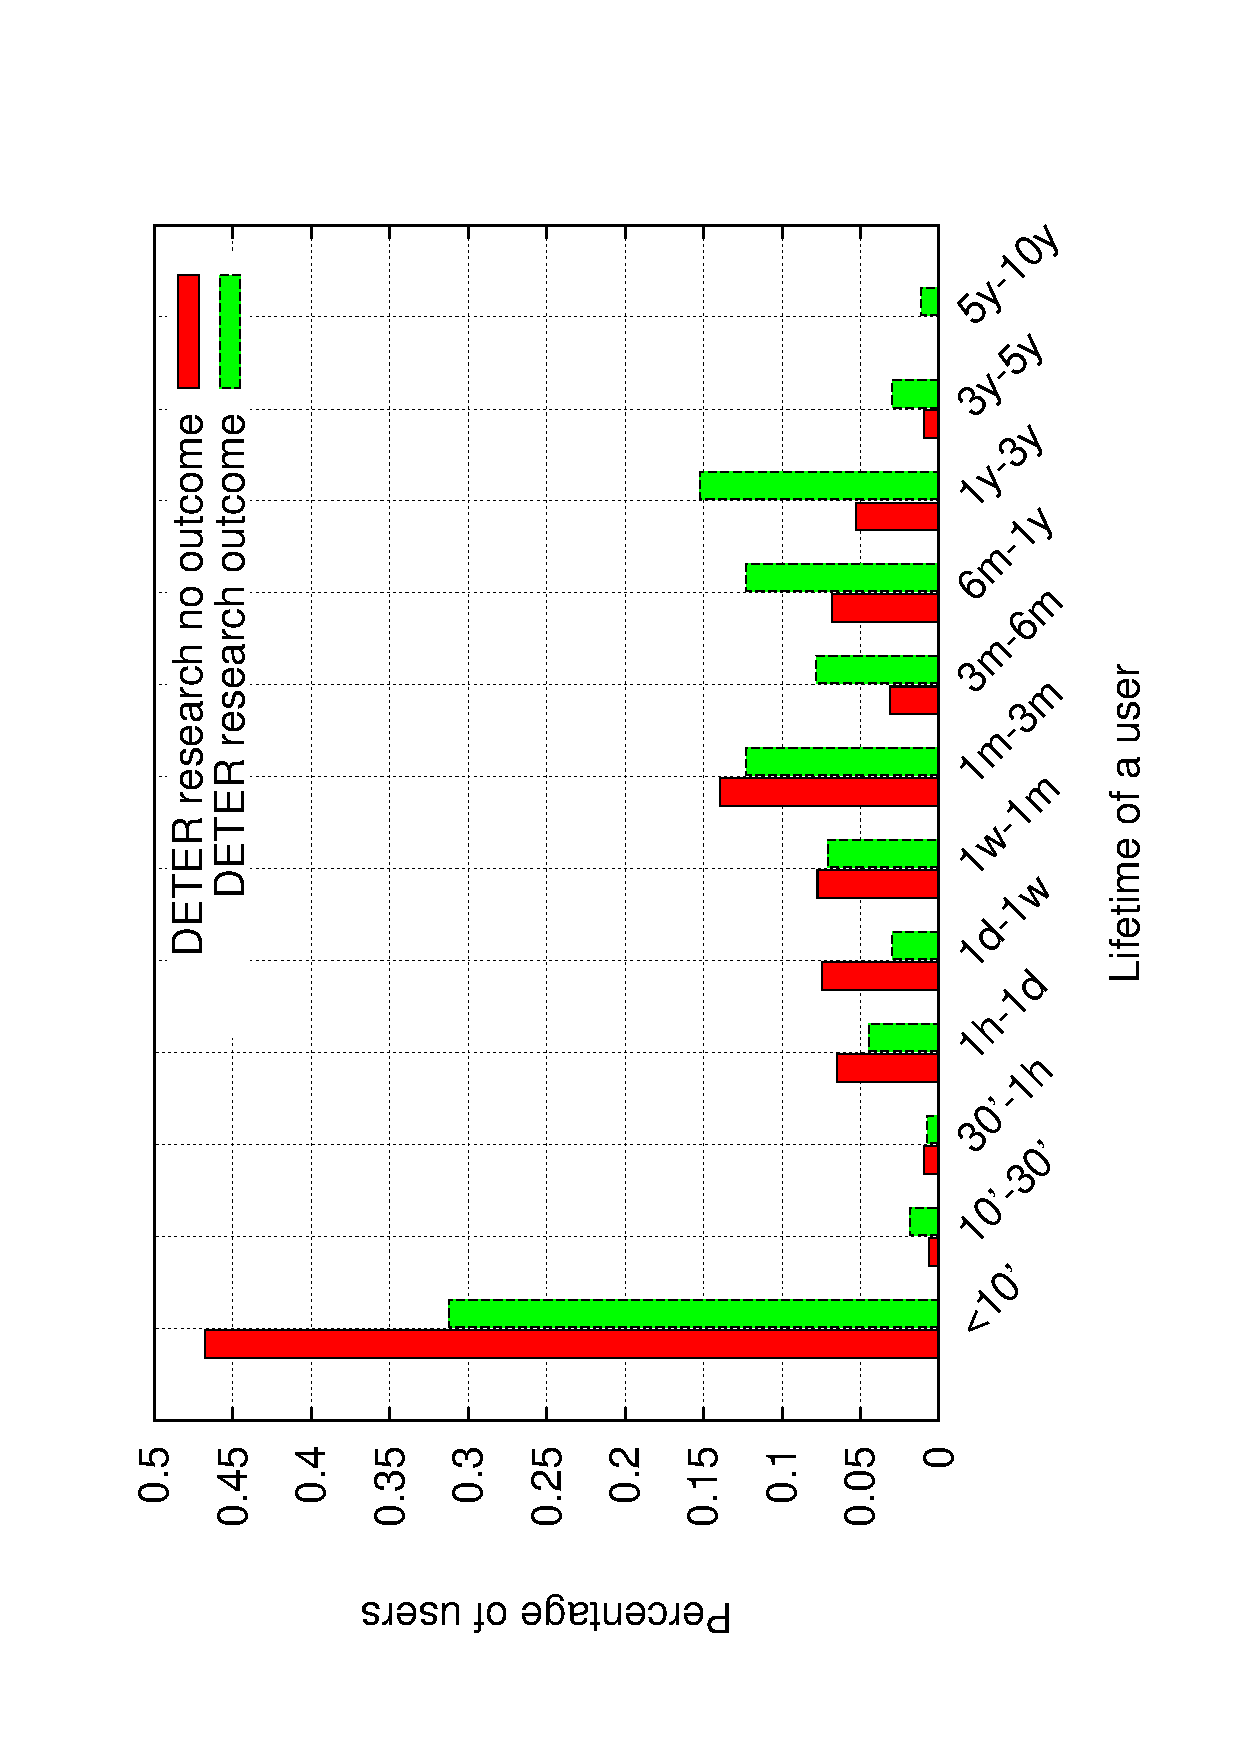
\includegraphics[width=3in,
type=pdf,ext=.pdf,read=.pdf]{figs/user.life.cmp.gnu} \caption{User
lifetime. Left: DETER vs Emulab, Right: All vs outcome} \label{userlife}
\end{center} \end{figure*}


\begin{figure*}[htbp] \begin{center} 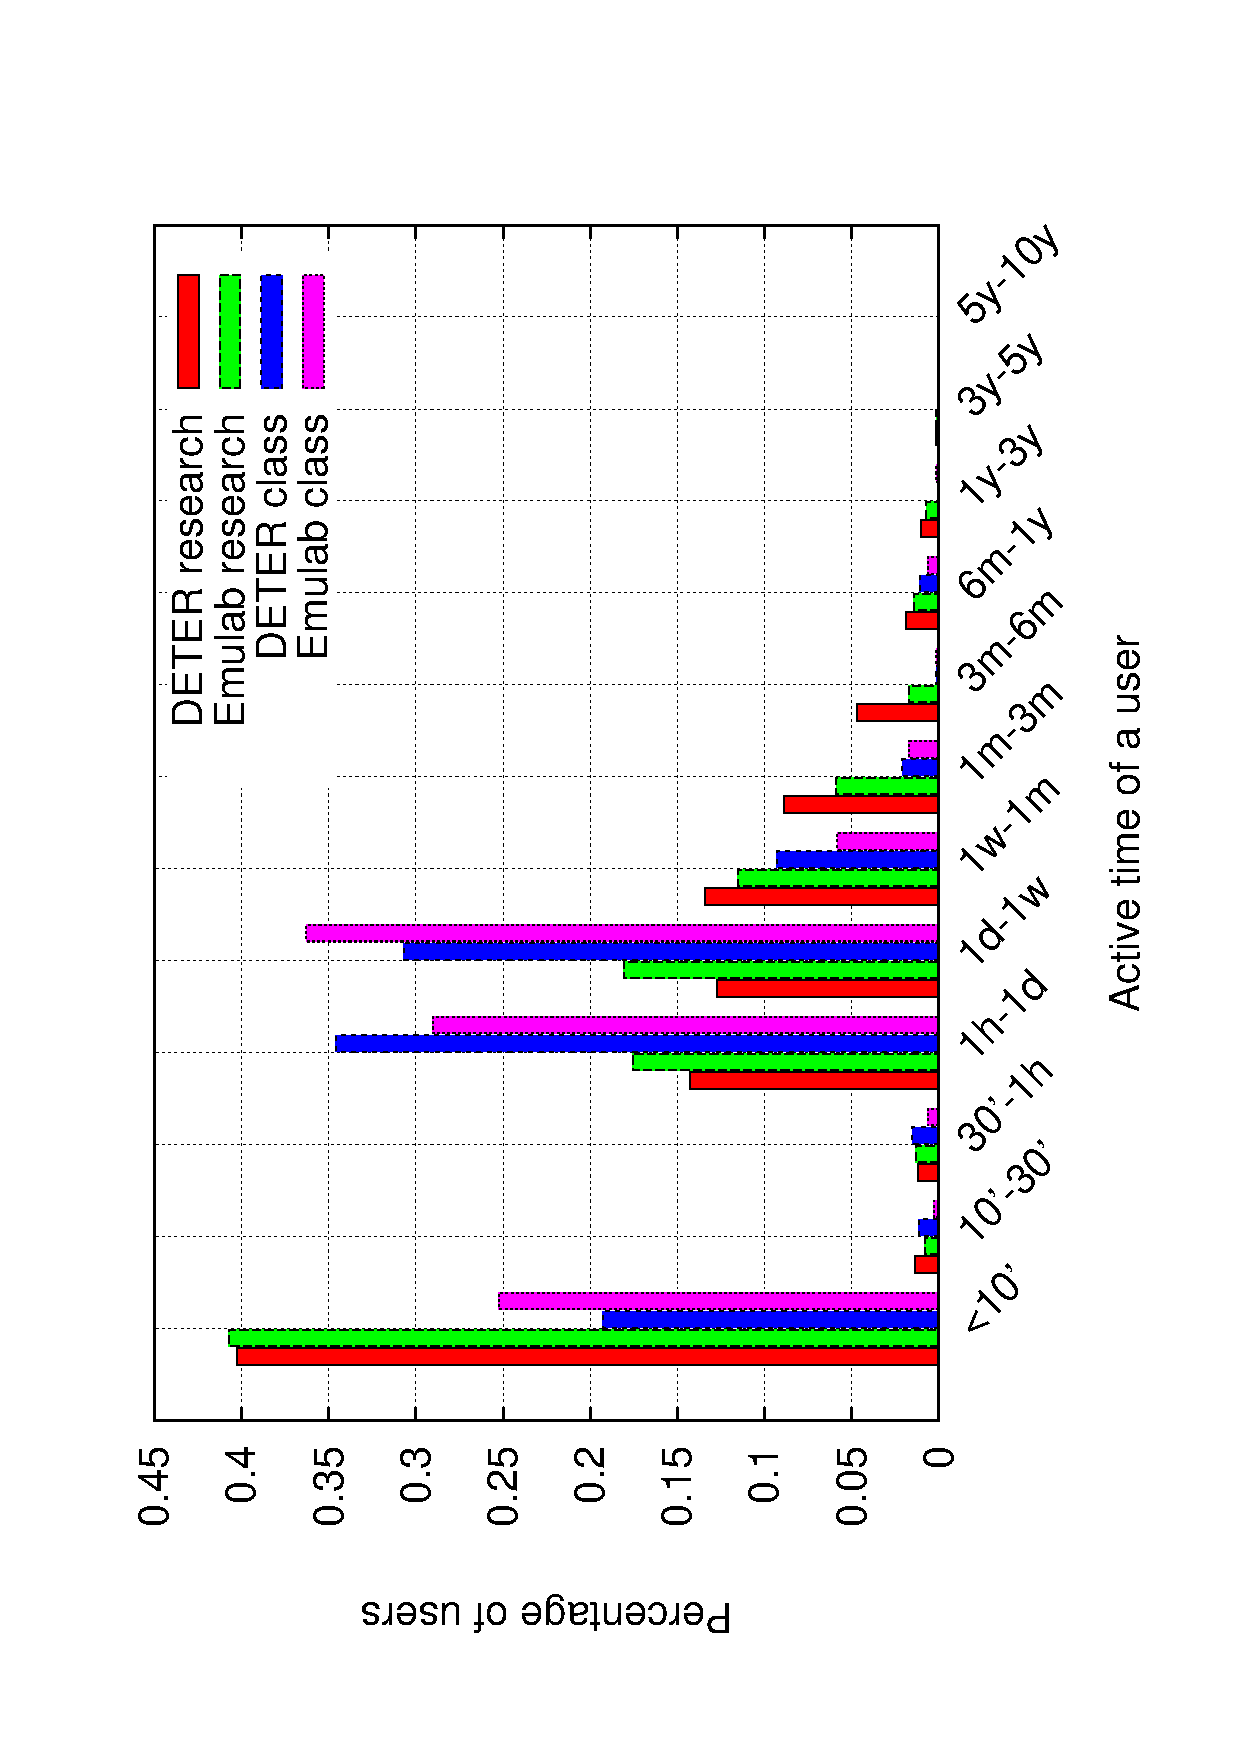
\includegraphics[width=3in,
type=pdf,ext=.pdf,read=.pdf]{figs/user.active.gnu}
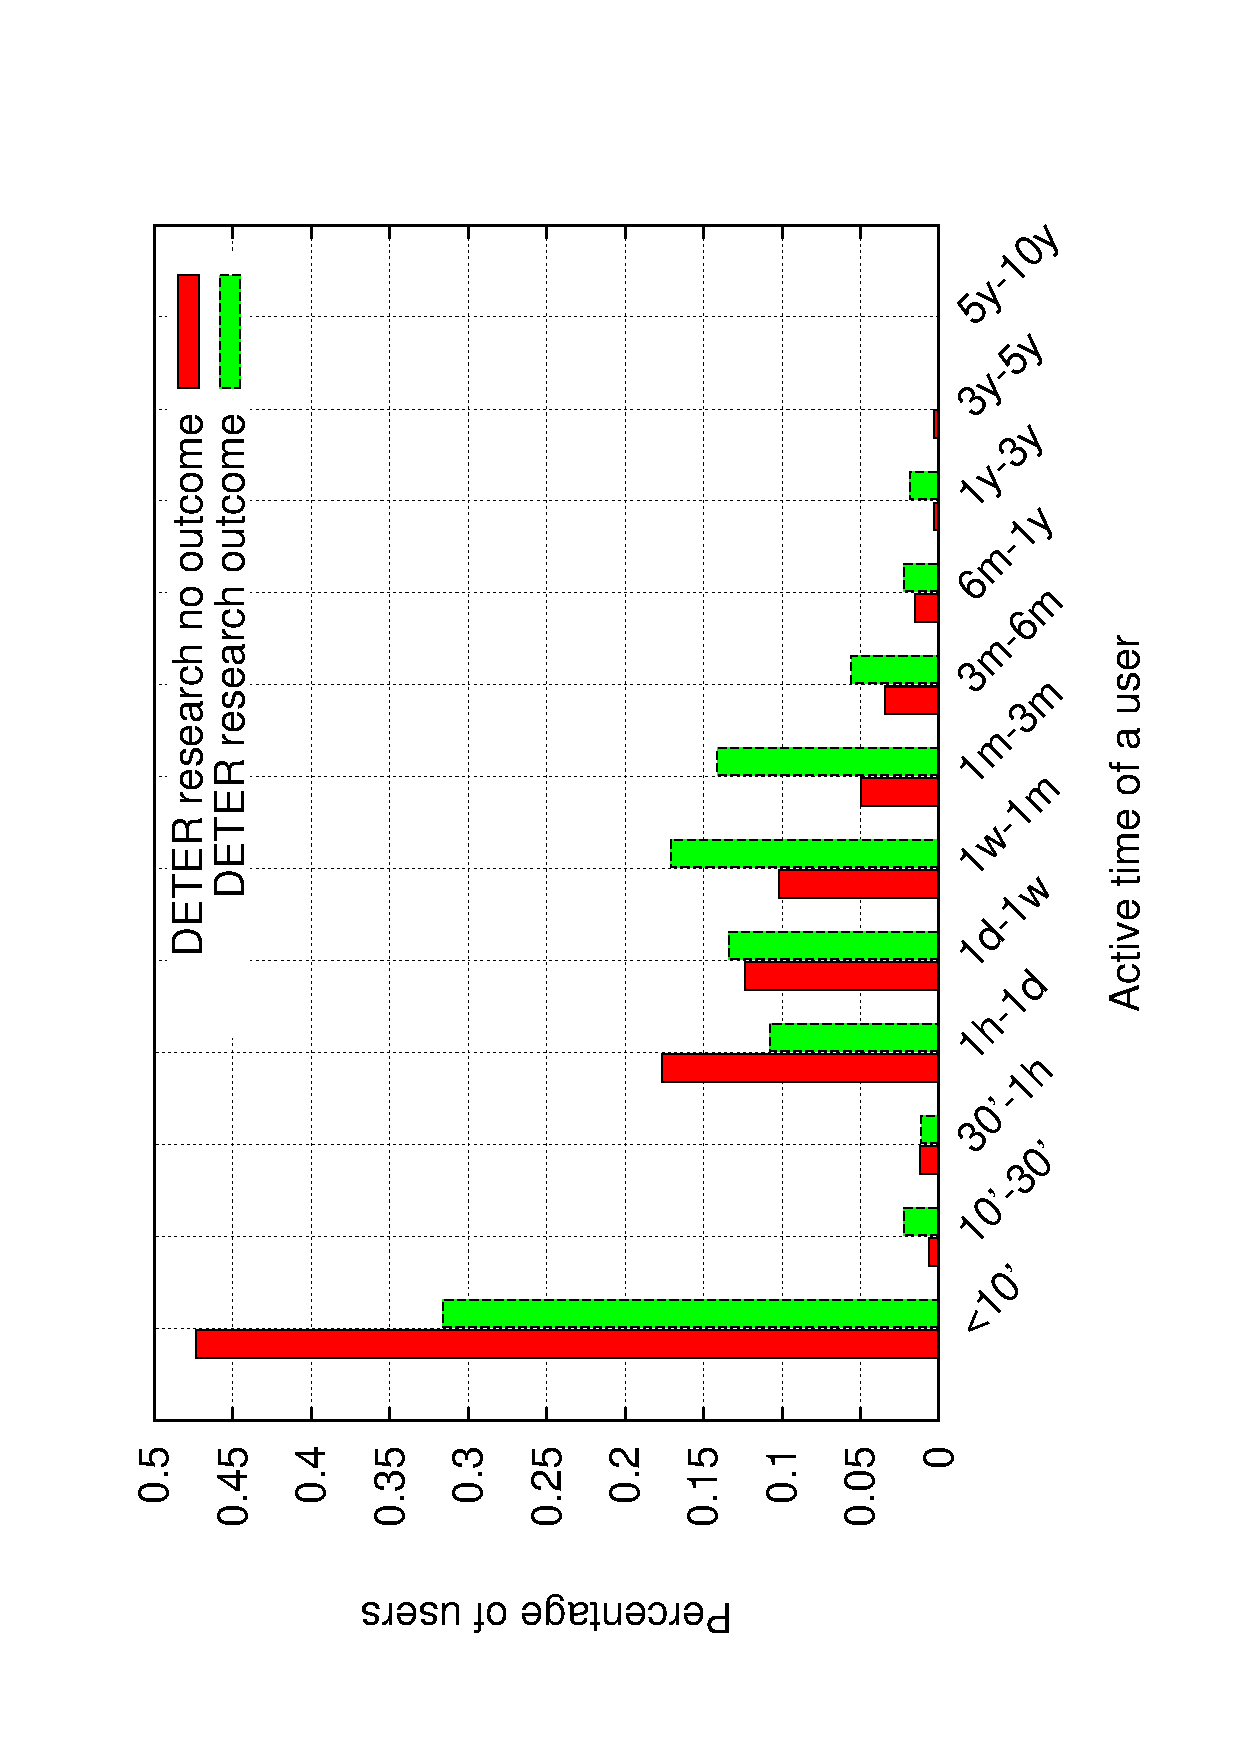
\includegraphics[width=3in,
type=pdf,ext=.pdf,read=.pdf]{figs/user.active.cmp.gnu} \caption{User
active time. Left: DETER vs Emulab, Right: All vs outcome}
\label{useractive} \end{center} \end{figure*}

\begin{figure*}[htbp] \begin{center} 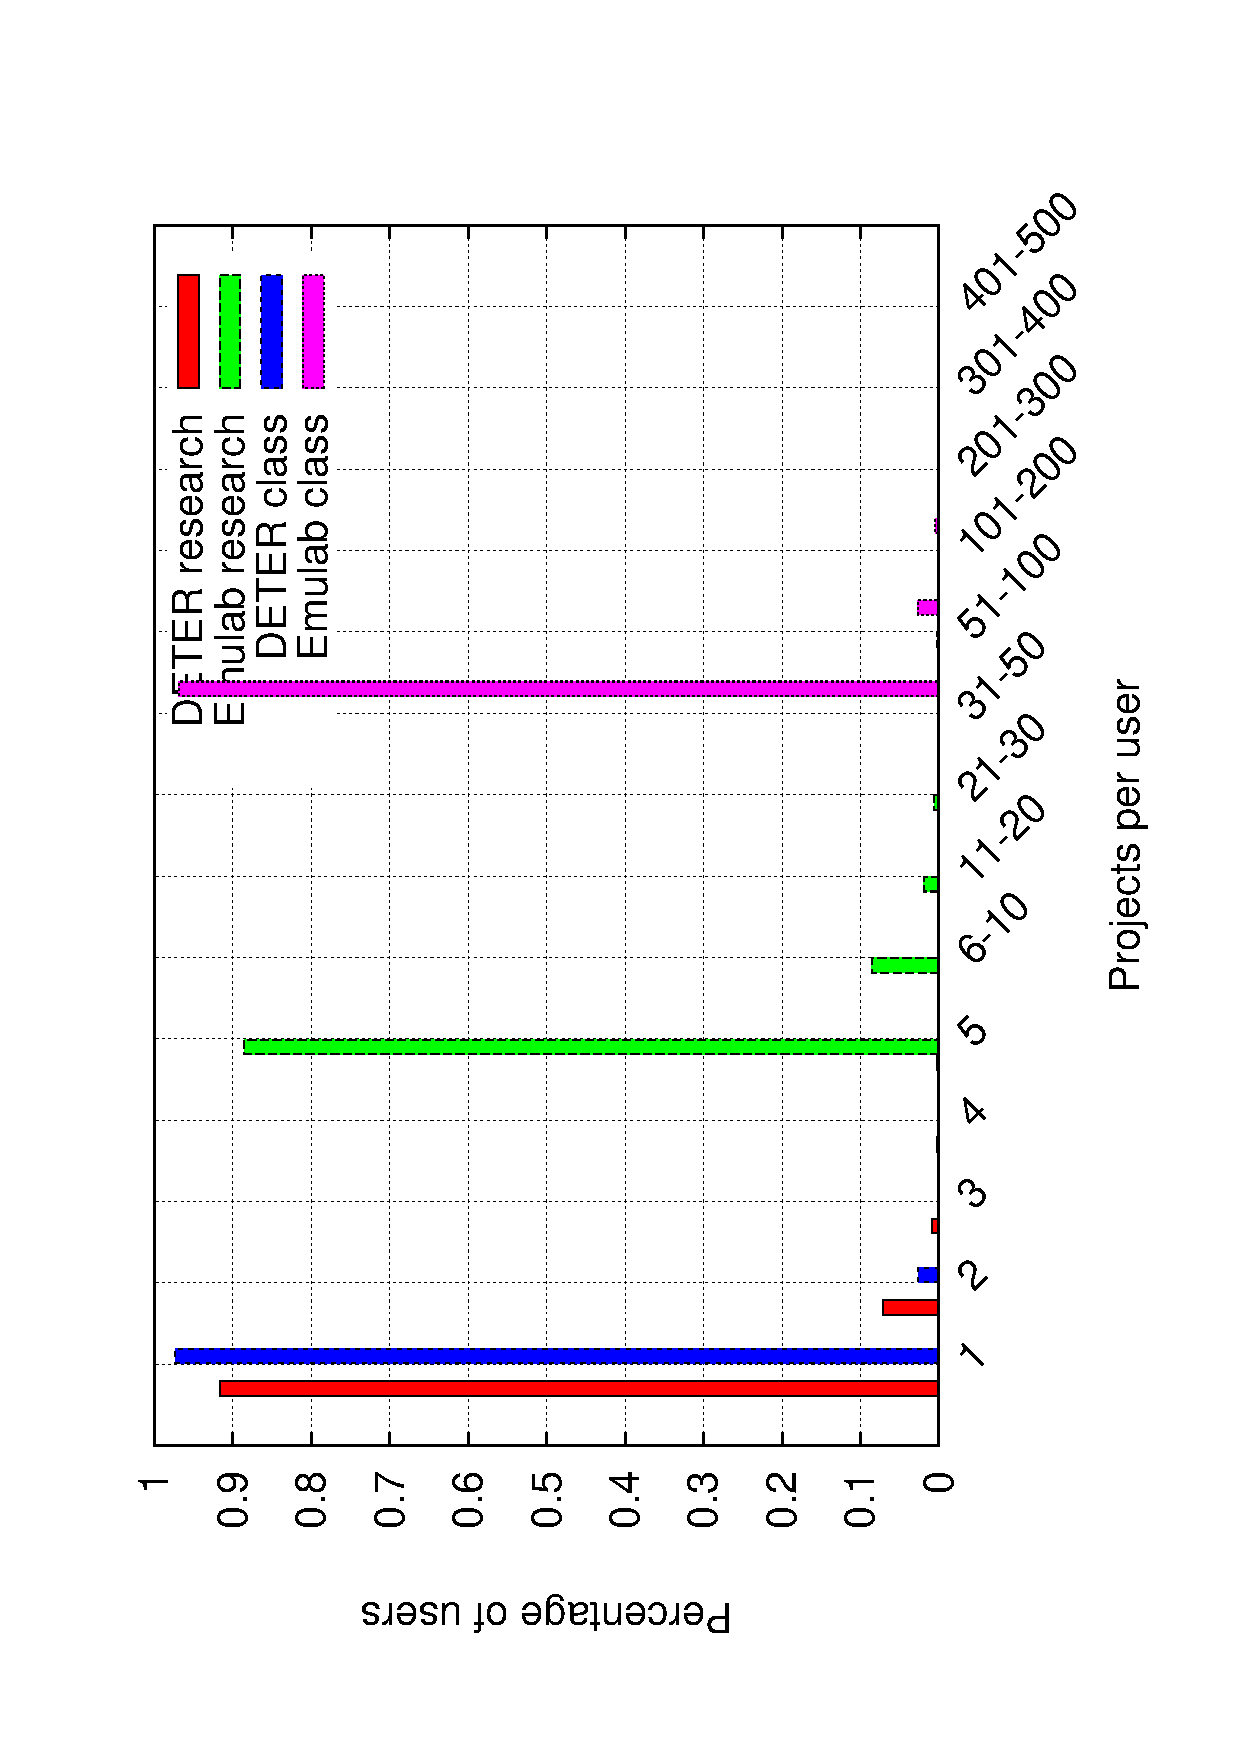
\includegraphics[width=3in,
type=pdf,ext=.pdf,read=.pdf]{figs/user.proj.gnu}
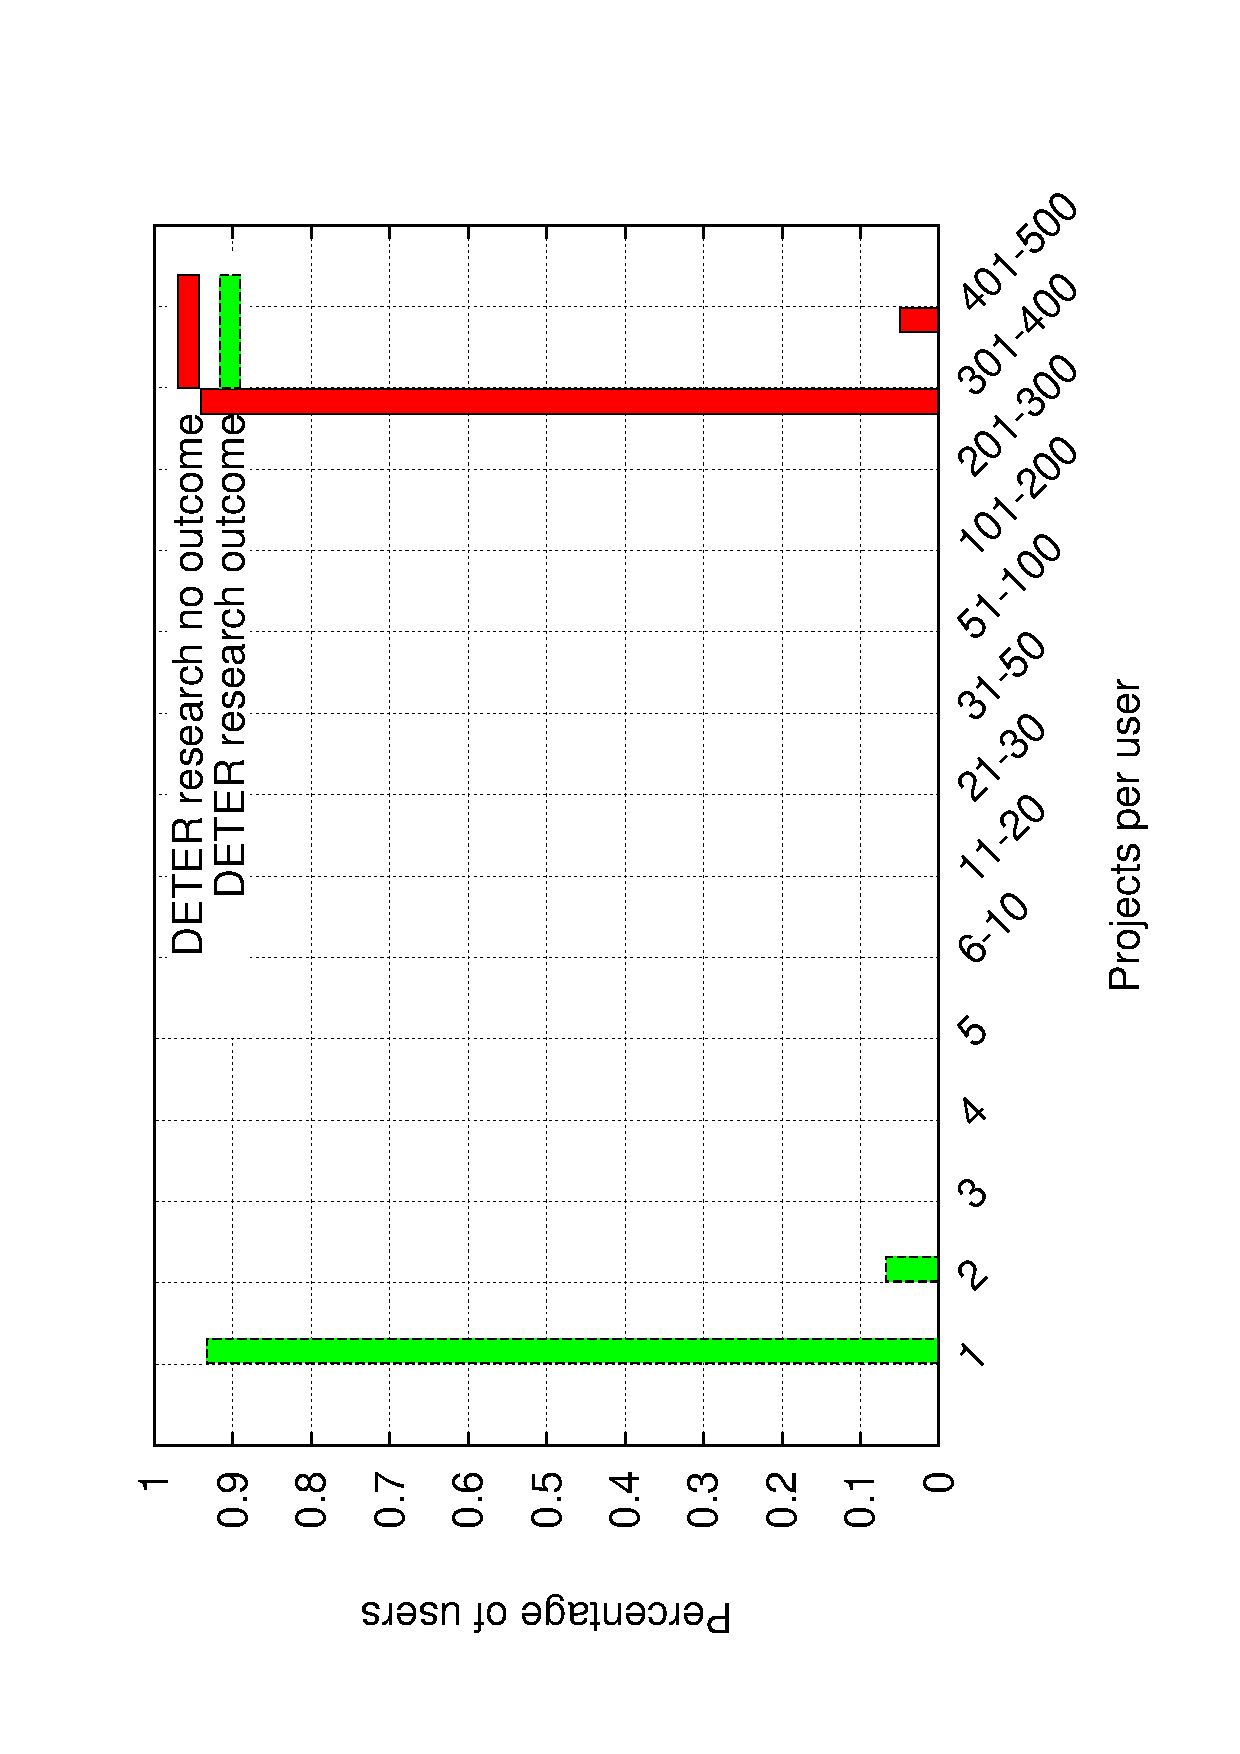
\includegraphics[width=3in,
type=pdf,ext=.pdf,read=.pdf]{figs/user.proj.cmp.gnu} \caption{Projects
per user. Left: DETER vs Emulab, Right: All vs outcome} \label{userproj}
\end{center} \end{figure*}

Members can be deleted and we don't account for that


\section{Idle Time}

\begin{table}[htdp] \caption{Node activity} \begin{center}
\begin{tabular}{|c|c|} \hline Activity & Percentage \\ \hline Idle &
57\% \\ Network & 30\% \\ CPU & 10\\ Interactive & 3 \\ \hline
\end{tabular} \end{center} \label{default} \end{table}%

57\% of timeslots reported by allocated node were idle but per
experiment all nodes are used together. There are really no huge
inactive periods so inactivity is spread through the experiment. 26\% of
timeslots report a network activity. 6.8\% report a CPU activity and 2\%
report a CPU and network activity.

\begin{figure*}[htbp] \begin{center} 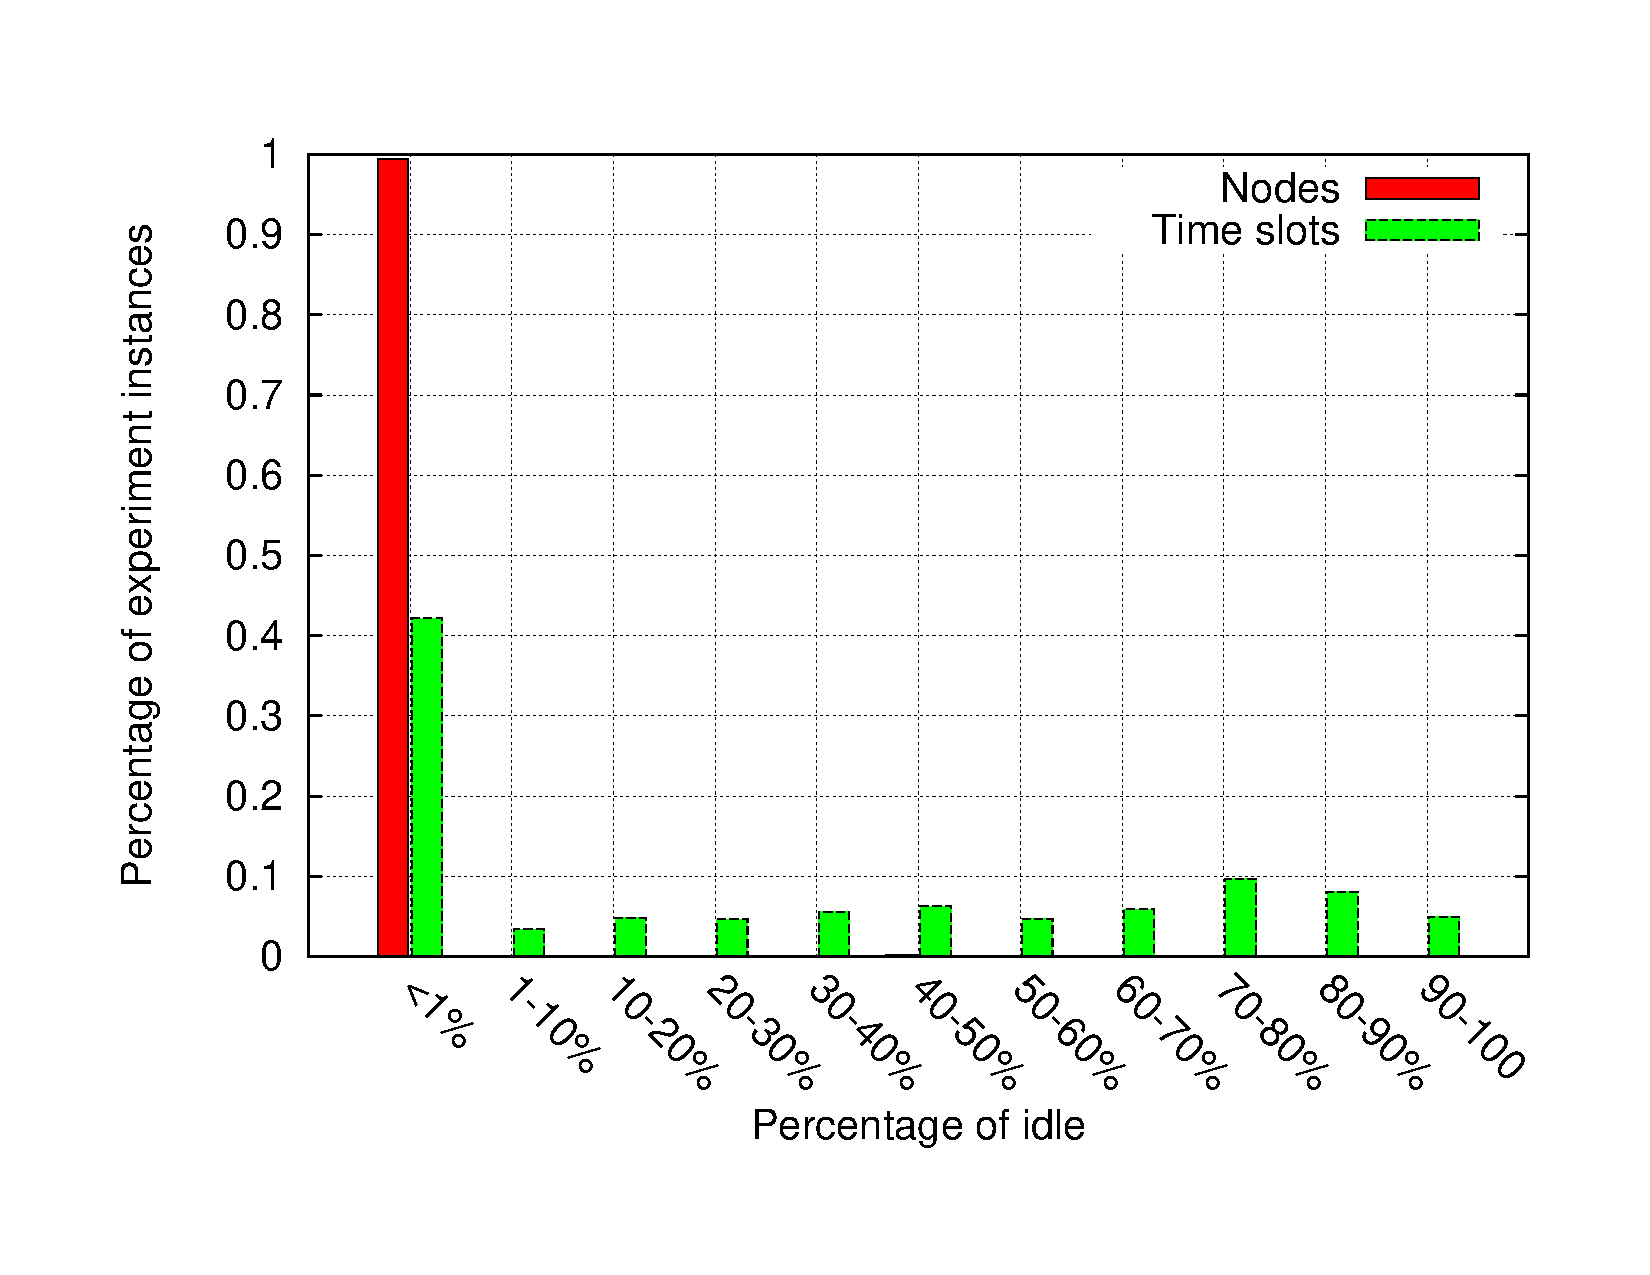
\includegraphics[width=3in,
type=pdf,ext=.pdf,read=.pdf]{figs/exp.idle.gnu}
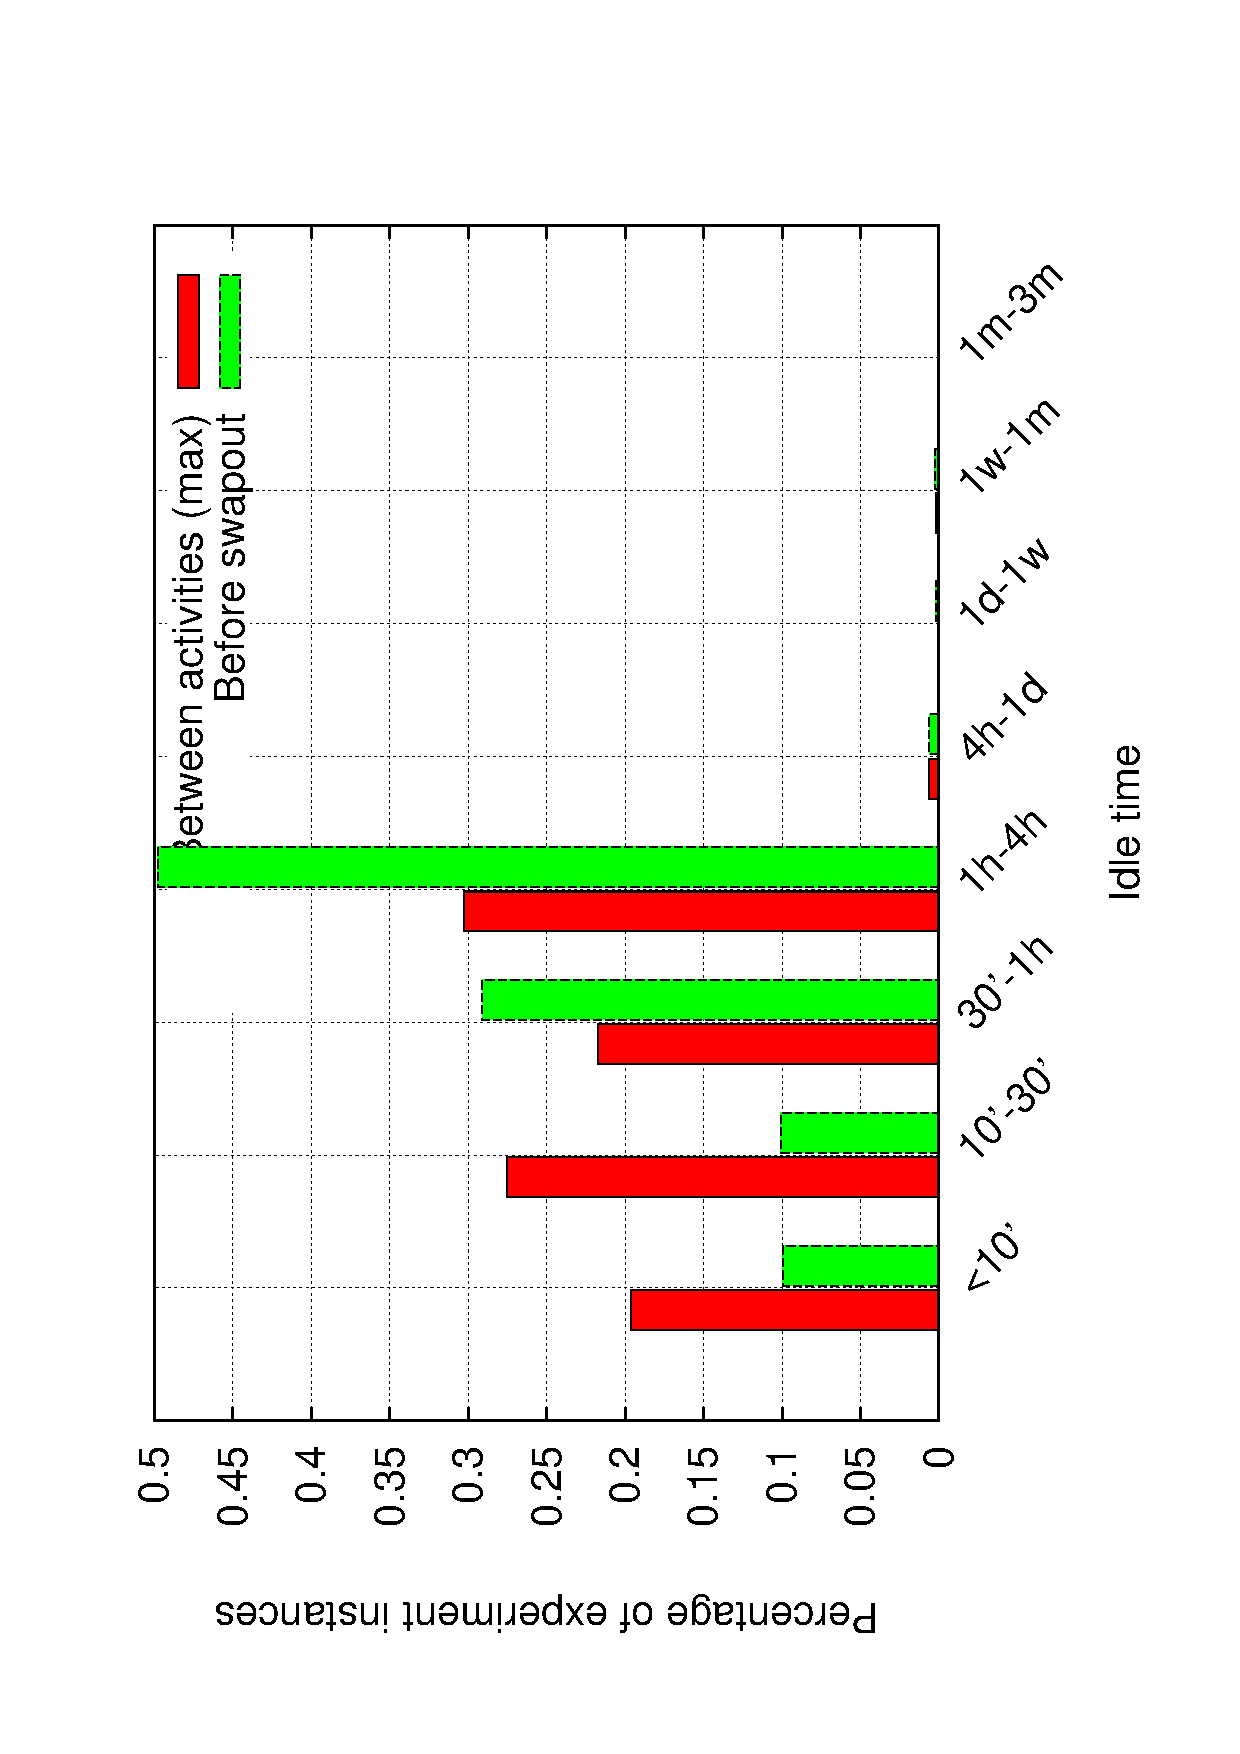
\includegraphics[width=3in,
type=pdf,ext=.pdf,read=.pdf]{figs/period.idle.gnu} \caption{Idleness per
experiment} \label{idle} \end{center} \end{figure*}


cummulative per project idle nodes correlate with experiment duration?
correlate with experiment history?

\section{Structural Patterns} 
\label{sec:topology}

% Hao 
All vs research/class vs research categories



\section{Testbed usage}

\begin{figure*}[htbp] \begin{center}
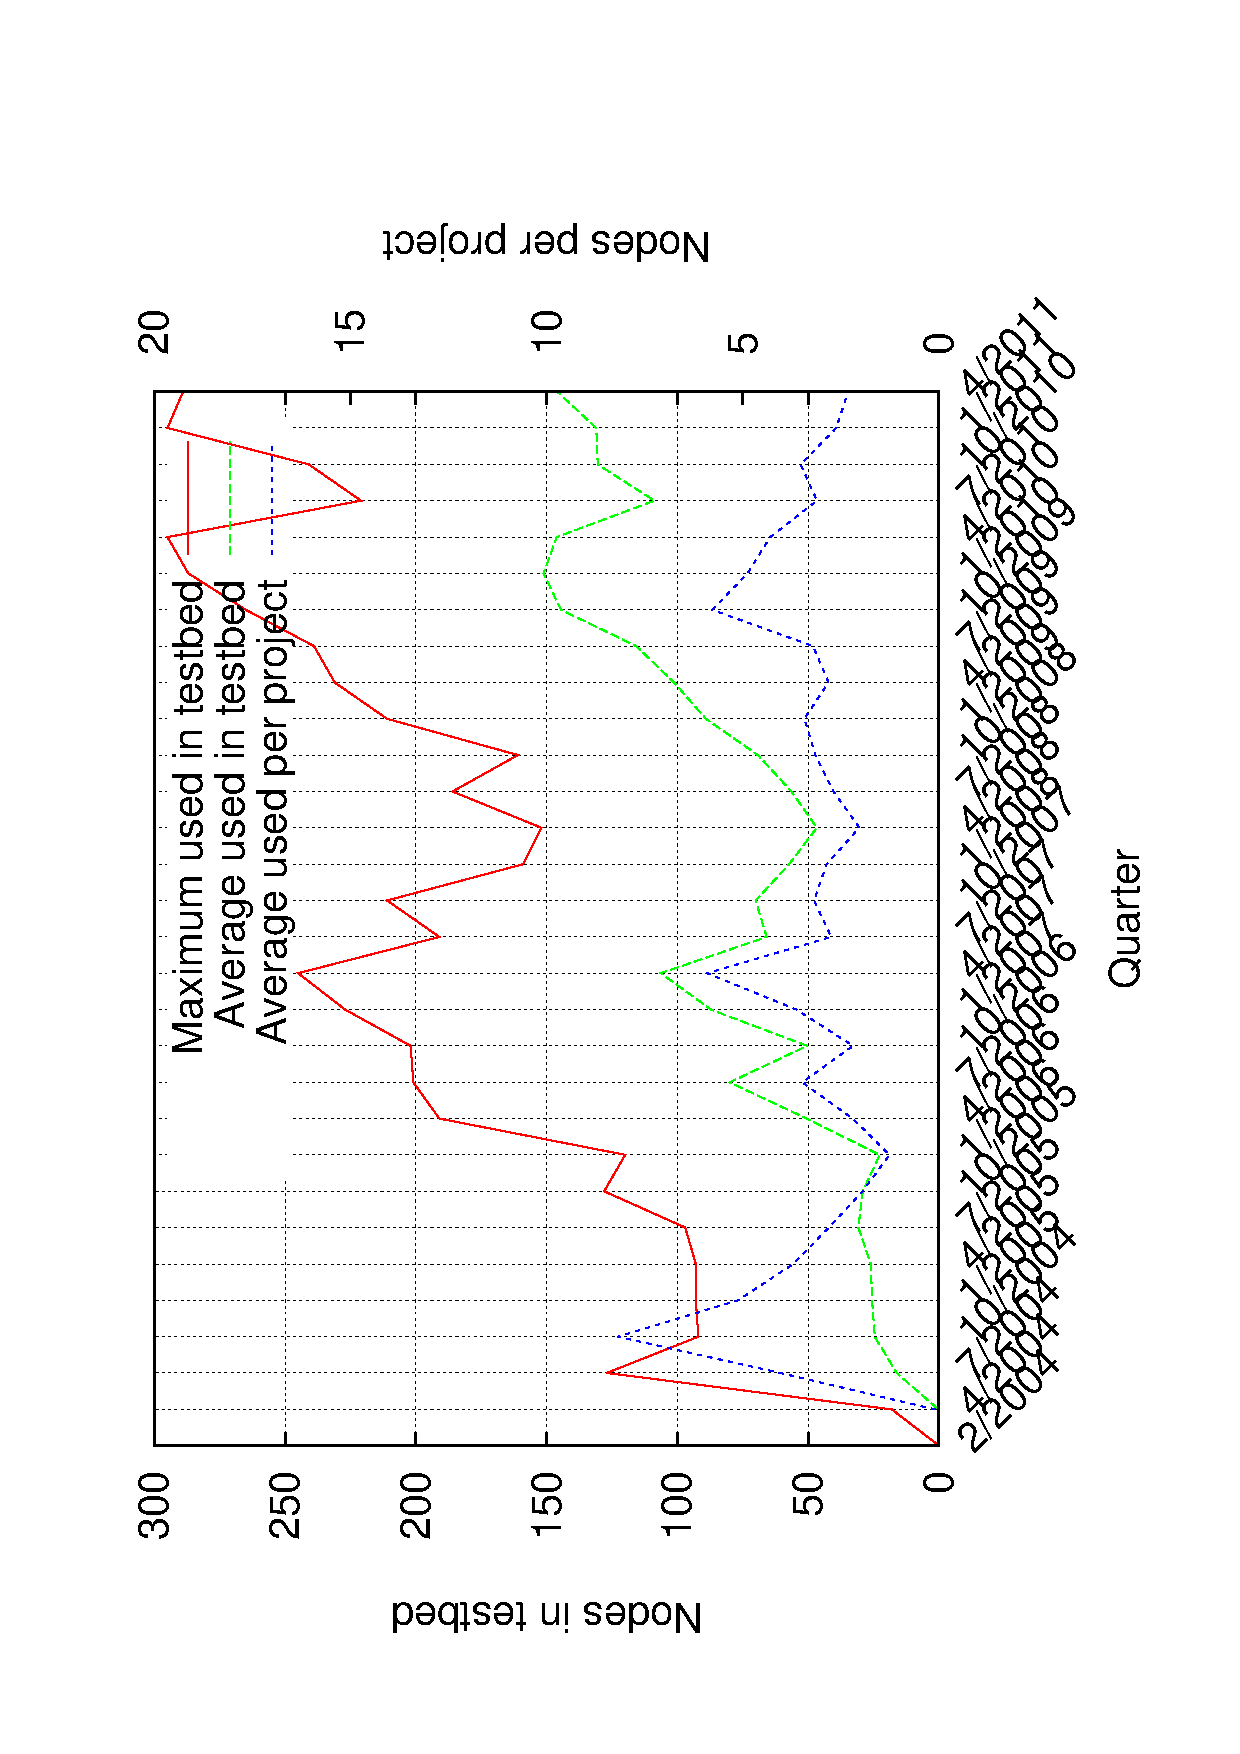
\includegraphics[width=3in,type=pdf,ext=.pdf,read=.pdf]{figs/nodes.gnu}
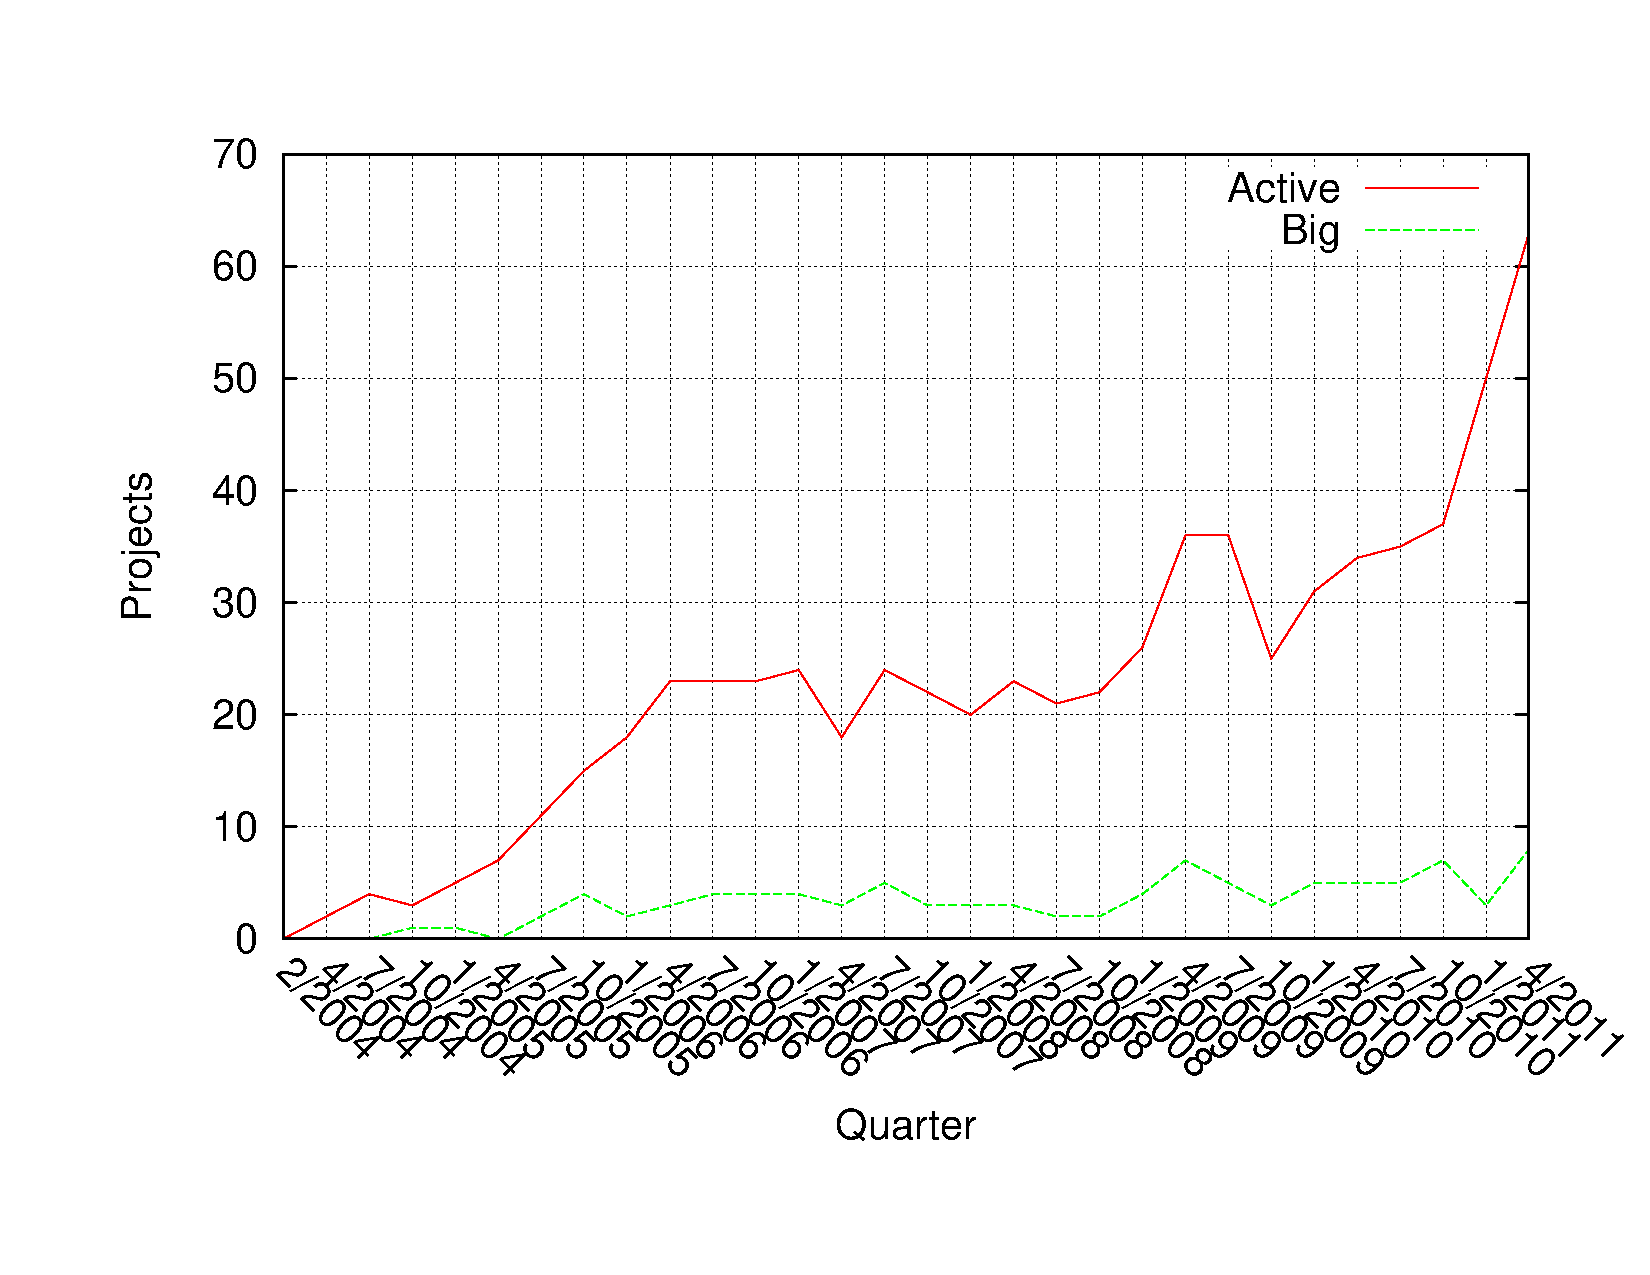
\includegraphics[width=3in,type=pdf,ext=.pdf,read=.pdf]{figs/projs.gnu}
\caption{Usage in node and project counts in DETER} \label{usagenp}
\end{center} \end{figure*}

\begin{figure*}[htbp] \begin{center}
\includegraphics[width=3in,type=pdf,ext=.pdf,read=.pdf]{figs/nodes.emu.
gnu}
\includegraphics[width=3in,type=pdf,ext=.pdf,read=.pdf]{figs/projs.emu.
gnu} \caption{Usage in node and project counts in Emulab}
\label{usagenpe} \end{center} \end{figure*}

\begin{figure*}[htbp] \begin{center}
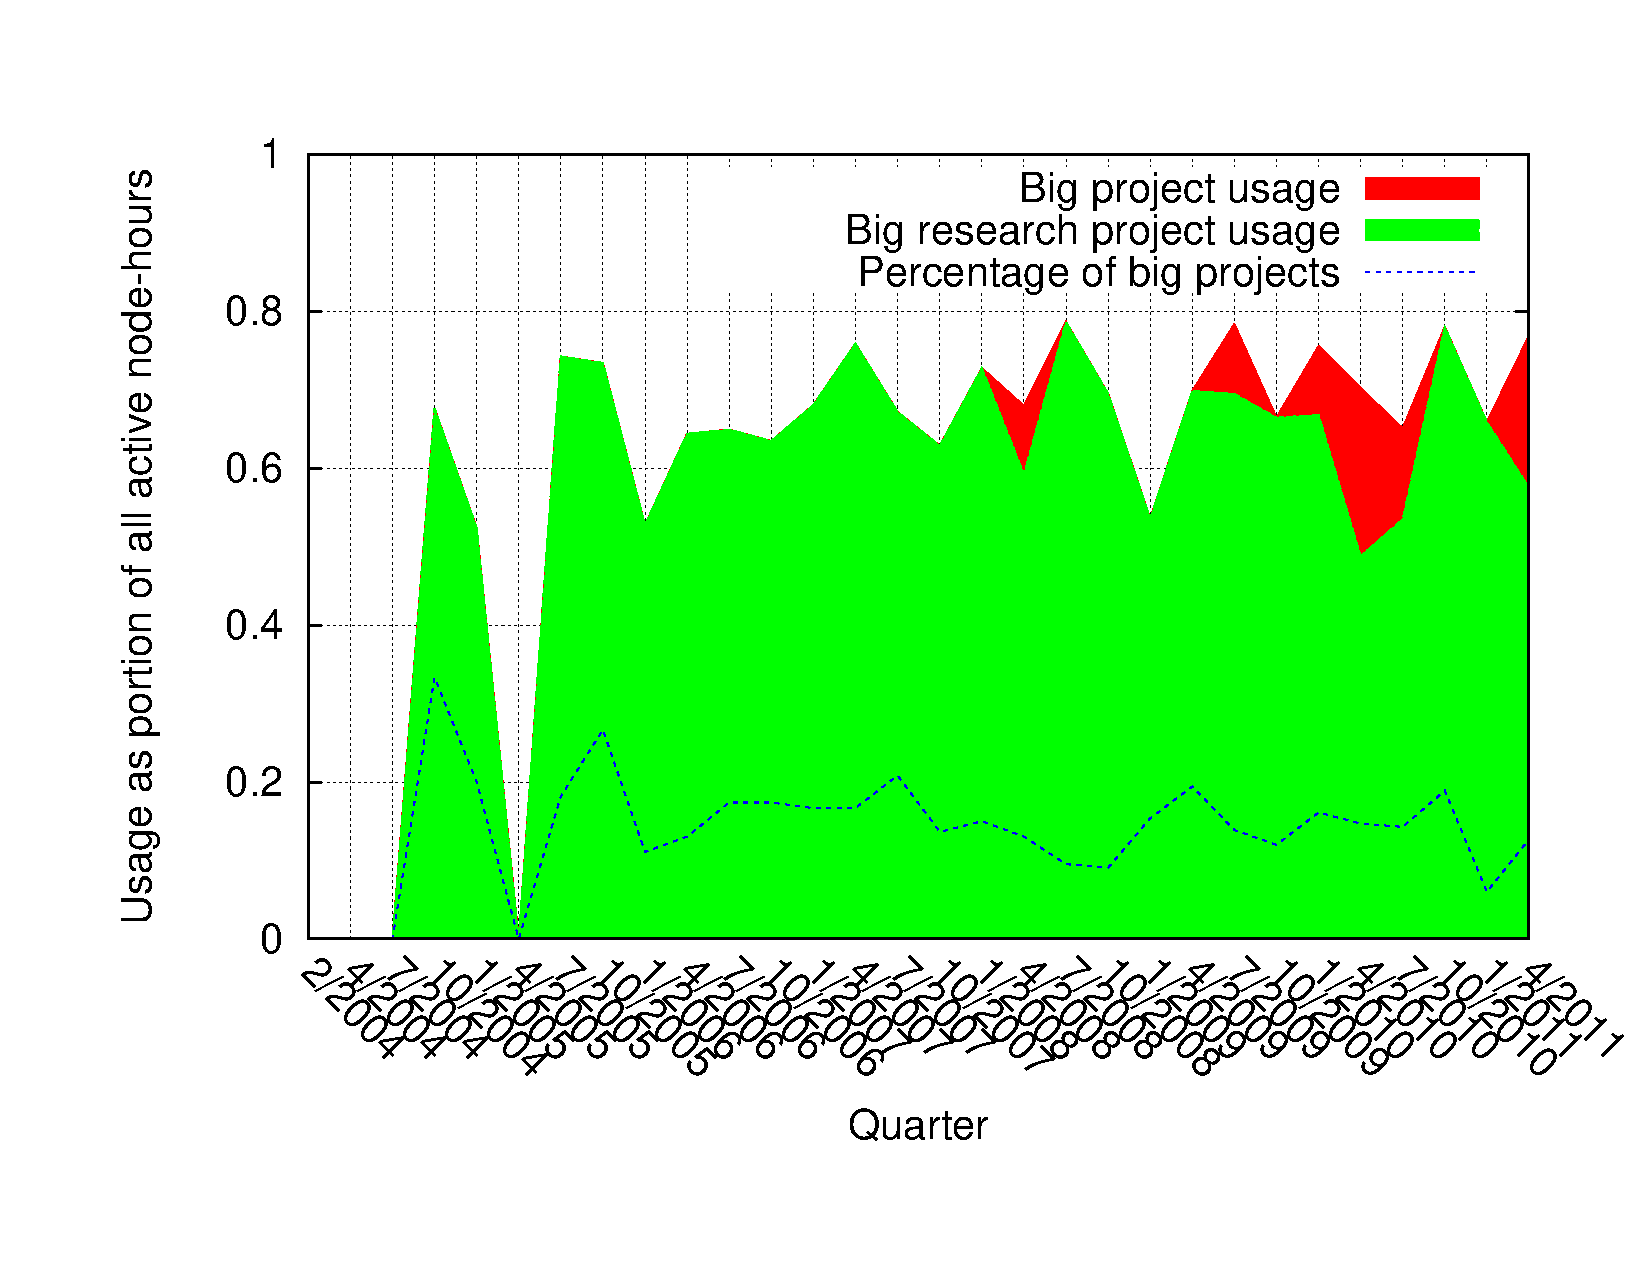
\includegraphics[width=3in,type=pdf,ext=.pdf,read=.pdf]{figs/usage.gnu}
\includegraphics[width=3in,type=pdf,ext=.pdf,read=.pdf]{figs/usage.
outcome.gnu} \caption{Usage dissection: big projects, research projects
and research projects with outcome in DETER} \label{usagedis}
\end{center} \end{figure*}

\begin{figure*}[htbp] \begin{center}
\includegraphics[width=3in,type=pdf,ext=.pdf,read=.pdf]{figs/usage.emu.
gnu}
\includegraphics[width=3in,type=pdf,ext=.pdf,read=.pdf]{figs/usage.
outcome.emu.gnu} \caption{Usage dissection: big projects, research
projects in Emulab} \label{usagedise} \end{center} \end{figure*}


\begin{figure*}[htbp] \begin{center}
\includegraphics[width=6in,type=pdf,ext=.pdf,read=.pdf]{figs/cat.usage.
gnu} \caption{Usage per project category in node-hours in DETER}
\label{catusage} \end{center} \end{figure*}

\begin{figure*}[htbp] \begin{center}
\includegraphics[width=6in,type=pdf,ext=.pdf,read=.pdf]{figs/cat.usage.
emu.gnu} \caption{Usage per project category in node-hours in Emulab}
\label{catusage} \end{center} \end{figure*}


experiment sizes and durations trends?

\section{User Survey}
\label{sec:survery} 

% we want more tools 
% want repositories to create start point and then build upon it 
% want full control but want to focus only on what is important to me 



\section{Looking Forward}
\label{sec:lfwd}

% tools, repositories
% support the complete experiment lifecycle 
% at-scale experimentaton 
% heterogeneous devices and diversity 




\section{Conclusion} 
\label{sec:conclusion}


\end{document}
